% -----------------------------------------------------------------------------
% Machine Intelligence II - the script.
% 
% current version modified in SS16 by Moritz Augustin
% -----------------------------------------------------------------------------

\documentclass[a4paper,11pt,titlepage]{article}

\usepackage[utf8]{inputenc}
\usepackage{amssymb,amsmath,amsfonts,mathrsfs,array}
\usepackage{enumerate,graphicx,fancyhdr,hyperref}
\usepackage[ruled]{algorithm2e}
%\usepackage{a4wide,wasysym} 
\usepackage{tikz,tkz-berge}
\usepackage{multirow,bigdelim}
\usepackage{mathtools}
\usepackage{commath}
\usetikzlibrary{arrows,topaths}
\hypersetup{pdfborder={0 0 0}} % links wont be visualized in the pdf
\usepackage{wrapfig}
\usepackage{subcaption}
\graphicspath{{../figures/pdf/}{../figures/png/}}
\pagestyle{fancy}

% ---------------------------- Page Headers (& footers)------------------------
\fancyhead[R]{\nouppercase{\rightmark}}

% --------------------- Equation Numbering-------------------------------------
\renewcommand {\theequation}{\thesection.\arabic{equation}}			
%\newcommand{\slideref}[1]{$\Box$\footnote{slide: #1}}
\newcommand{\slideref}[1]{\marginpar{$\Box$\parbox{1.25cm}{\centering\tiny #1}}}


% ------------------------- New Commands --------------------------------------
\newcommand{\eqexcl}{\ensuremath{\stackrel{\mathrm{!}}{=}}}
\newcommand{\corresponds}{\ensuremath{\widehat{=}}}
\newcommand{\coloneqq}{\ensuremath{:=}}
\newcommand{\argmin}{\operatornamewithlimits{argmin}}
\newcommand{\sign}{\operatorname{sign}}
\newcommand{\emp}{\operatorname{emp}}
\newcommand{\dkl}{D_{KL}}
\newcommand{\dvc}{\mathrm{d}_{\mathrm{VC}}}
\newcommand{\argmax}{\operatornamewithlimits{argmax}}
\newcommand{\itr}{\item[$\rightarrow$]}
\newcommand{\itR}{\item[$\Rightarrow$]}
\newcommand{\itl}{\item[$\leadsto$]}
\newcommand{\kurt}{\operatorname{kurt}}
\newcommand{\var}{\operatorname{var}}
\newcommand{\ra}{$\rightarrow\;$}

% matrices with different types of brackets 
\newcommand{\mat}[2][rrrrrrrrrrrrrrrrrrrrrrrrrr]{
  \left[ \begin{array}{#1} #2\\ \end{array} \right]}
\newcommand{\rmat}[2][rrrrrrrrrrrrrrrrrrrrrrrrrr]{
  \left( \begin{array}{#1} #2\\ \end{array} \right)}
\newcommand{\dmat}[2][rrrrrrrrrrrrrrrrrrrrrrrrrr]{
  \left|\left[ \begin{array}{#1} #2\\ \end{array} \right]\right|}
\newcommand{\drmat}[2][rrrrrrrrrrrrrrrrrrrrrrrrrr]{
  \left|\left( \begin{array}{#1} #2\\ \end{array} \right)\right|}
\renewcommand{\vec}[1]{\ensuremath{\underline{\mathbf{#1}}}}
% NOTE: Vector notation used in neural network textbooks -- this is 
% easier to read for expressions like \hat{\underline{\mathbf{w}}}. 



\lhead{Machine Intelligence II}
\title{Machine Intelligence II\\\rule{0.75\textwidth}{2pt}}
\author{Prof. Dr. Klaus Obermayer}

%\date{}	

\usepackage[backend=biber,style=authoryear,natbib=true, url=false, doi=true, firstinits=true, eprint=false]{biblatex}
\addbibresource{referencesMI2.bib}

%%\includeonly{section3}
% -----------------------------------------------------------------------------
\begin{document}
\maketitle
\noindent \textcolor{red}{\underline{Disclaimer:} The lecture has been restructured in the previous terms (SoSe 2017 as well as SoSe 2018) and several new topics were added (and are being added), too. Many of these changes are so far only reflected in the lecture slides but not yet in these lecture notes which are thus outdated. Although we plan to complete the lecture notes soon, it is unlikely that we reach this goal until the end of the term. Therefore, it is strongly recommended to make hand-written notes within the lectures to complement the information of this script. We apologize for the inconvenience.}
\newpage
\tableofcontents
\newpage

% ----------------------  Main Text  -----------------------------------------
% old topic order was (before SS13 or so): 
% 1) densitiy estimation first
% 2) projection
% 3) stoch opt.
% 4) clustering/embedding
% however, figures etc have the old section number so recommendation is to keep internally 
% the old enumeration

\setcounter{section}{-1}
\section{Introductory comments}

Methods subsumed under the term \emph{unsupervised learning} deal with
finding structure or regularities in a set of observations
$\vec{x}^{(1)}, \vec{x}^{(2)}, \ldots,\vec{x}^{(p)}$.


\paragraph{What is the statistical structure of the data?} \mbox{}\\\\
Many datasets ...
\begin{itemize}
\item[...] are high-dimensional \ra visualization \& dimension reduction
\item[...] are grouped or clustered \ra definition of groups / categories, construction of taxonomies, preprocessing for prediction (clustering)
\item[...] may display interesting (or uninteresting) directions \ra
  definition of ''informative'' features (projection methods)
\item[...] may be determined by different causes \ra unmixing a mixture of sources, definition
  of components, infering causes
\end{itemize}

\paragraph{Motivation:} 
In contrast to methods of \emph{supervised learning} (see MI1), there
is no additional information in terms of ``labels''
$\vec{y}^{(\alpha)}$ providing a ``correct'' classification or target
value for data point $\alpha$.
\\\\
The statistical structure of a data set is often interesting in itself
and can be exploited for knowledge extraction (modeling).
Furthermore, it allows to find new representations of the data
$\vec{x}$ that allow more efficient data storage ($\leadsto$
dimensionality reduction, data compression) or are better suited to
solve supervised problems such as prediction, classification,
reasoning, decision making.

\paragraph{Unsupervised learning \& statistical data analysis:}
methods for the extraction of the statistical ''structure'' underlying
a set of observations (or a data structure)
\begin{itemize}
	\itR projection methods: search for ''interesting'' directions in 
		feature space
	\itR clustering methods: grouping \& categorization (and prototypes)
\end{itemize}
\emph{Note:} Both PCA and ICA (discussed in chapters \ref{sec:PCA} and
\ref{sec:ICA}) are linear projection methods.  In many
cases (e.g.\ PCA) kernel methods allow to extend them to nonlinear
problems.
 %% Introductory comments: Unsupervised Learning
%% see also NotesICA.tex in SS2013
%% add matrix version to PCA methods (see handwritten notes in script)?

\newpage 						% for visual reasons
\section{Projection Methods}
Projection methods provide important tools for high-dimensional datasets
\begin{figure}[h]
  \centering
  \begin{tabular}{c c}
    \raisebox{-2cm}{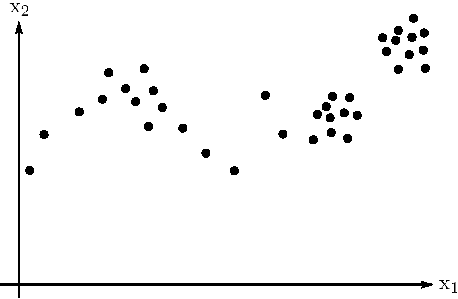
\includegraphics[width=5cm]{section2_fig1}} & 
    \parbox{5.6cm}{$p$ observations with $N$ dims.:\\ 
    $\big\{ \vec{x}^{(1)}, \; \vec{x}^{(2)}, \; \ldots, \; \vec{x}^{(p)} \in \mathbb{R}^N \big\}$}
%     $\big\{ \vec{x}^{(\alpha)} \big\}, \alpha = 1, \ldots, p; \quad \vec{x}^{(\alpha)} \in \mathbb{R}^N$}
  \end{tabular}
  \caption{Projection and clustering methods for multidimensional data}
  \label{tab:scenario-proj-meth}
\end{figure}



\subsection{Principal Component Analysis}\label{sec:PCA}
% -----------------------------------------------------------------------------

\subsubsection{The Covariance Matrix}
observations: $\big\{ \vec{x}^{(\alpha)} \big\}, \; \alpha = 1, \ldots, p; \quad \vec{x}^{(\alpha)} \in \mathbb{R}^N$
\\\\
{\bf Feature space:}
\begin{figure}[h]
  \centering
  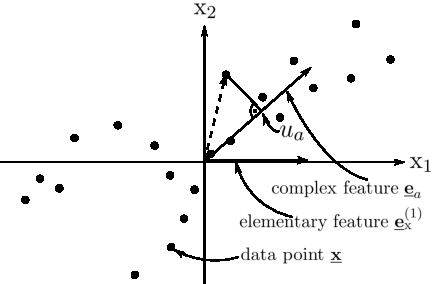
\includegraphics[width=8cm]{section2_fig2}  
  \caption{Data, elementary and complex features}
  \label{fig:features}
\end{figure}
\begin{figure}[h]
  \centering
  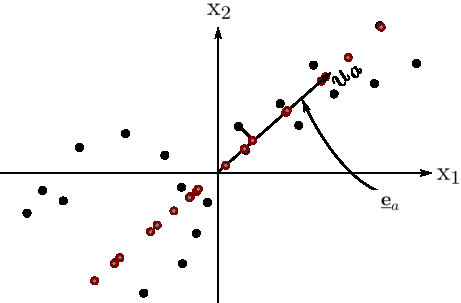
\includegraphics[width=8cm]{section2_fig2b}  
  \caption{Same data as in Fig.~\ref{fig:features}, projected onto complex feature $\vec{e}_a$ with feature values $u_a$}
  \label{fig:featuresproj}
\end{figure}
\begin{description}
\item[elementary features $\vec{e}_\mathrm{x}^{(1)}, \vec{e}_\mathrm{x}^{(2)}, \vec{e}_\mathrm{x}^{(3)}, \ldots \vec{e}_\mathrm{x}^{(N)}$:] basis vectors of unit length which correspond to the individual measurements
\item[complex feature $\vec{e}_a$:] vector of unit ($\|\vec{e}_a\|=1$) length which
  corresponds to a particular direction in feature space
\item[feature value $u_a$:] projection of observation $\vec{x}$ onto the complex feature $\vec{e}_a$
\end{description}
\begin{equation}
	\underbrace{u_a }_{ \text{{\small value}} }
	= \underbrace{ \vec{e}_a^T }_{ \text{{\small feature}} }
	\cdot \underbrace{ \vec{x} }_{ \text{{\small observation}} }
\end{equation}


\paragraph{Example -- Leptograpsus data:} Dead crabs lose their color and their sexual features -- 
Can we infer species / sex from the shells alone?
\[ \text{crabs: L. variegatis} \left\{ \begin{array}{l}
		\text{orange} \\\\
		\text{blue}
	\end{array} \right. \left\} \begin{array}{l}
		\text{two (sub-)species} \\\\
		\rightarrow \text{ male and female crabs}
	\end{array} \right.
\] \slideref{Ex: More examples on slide\\Leptograpsus data, Iris data}

\begin{itemize}
\item \emph{elementary features: }
\[ \left. \begin{array}{ll}
	\text{width of the frontal lip:} & \mathrm{x}_1 \\
	\text{width of the back:} & \mathrm{x}_2 \\
	\text{length along midline:} & \mathrm{x}_3 \\
	\text{max. width of top shell:} & \mathrm{x}_4 \\
	\text{body depth:} & \mathrm{x}_5
\end{array} \right\} \text{5-dim. feature vector} \]
\item \emph{complex features:} some direction in feature space (i.e.\ linear combination of elementary features) which is indicative of color and/or sex.
\end{itemize}

\paragraph{Moments of the set of observations:} Moments of a distribution provide important information about the location and shape of a distribution.
\\\\
First moment (sample mean/center of mass):
\begin{equation}
	\vec{m} = \frac{1}{p} \sum\limits_{\alpha = 1}^p \vec{x}^{(\alpha)}
\end{equation}
Second moments (Variances and Covariances):
\begin{equation}
	C_{ij} = \frac{1}{p} \sum\limits_{\alpha = 1}^p 
		\underbrace{ \Big( \mathrm{x}_i^{(\alpha)} - m_i \Big) }_{
			\substack{	\text{deviations from} \\
					\text{the mean}} }
		\underbrace{ \Big( \mathrm{x}_j^{(\alpha)} - m_j \Big) }_{
			\substack{	\text{component} \\
					\text{indices } i,j}}
\end{equation}
In vector notation:
\begin{equation} \tag{covariance matrix}
	\vec{C} = \frac{1}{p} \sum\limits_{\alpha=1}^p 
		  \left ( \vec{x}^{(\alpha)} - \vec{m} \right ) \left ( \vec{x}^{(\alpha)} - \vec{m} \right )^T
		% =   \big\{ C_{ij} \big\}
\end{equation}
\textbf{Note:} ''Centering'' the data\footnote{centering: subtract mean from all data points} yields
$\vec{m} = \vec{0}$ and we obtain
\begin{equation}
	C_{ij} = \frac{1}{p} \sum\limits_{\alpha = 1}^p \mathrm{x}_i^{(\alpha)}
			\mathrm{x}_j^{(\alpha)}
\end{equation}
and thus 
\begin{equation}
	\vec{C} = \frac{1}{p} \sum\limits_{\alpha=1}^p 
		   \vec{x}^{(\alpha)}\left ( \vec{x}^{(\alpha)}\right )^T
		% =   \big\{ C_{ij} \big\}
\end{equation}

\paragraph{Properties of the covariance matrix}
\[ \begin{array}{ll}
	C_{ij} = C_{ji}
	& \text{the covariance matrix is symmetric} \\\\
	i = j
	& C_{ii} = \frac{1}{p} \sum\limits_{\alpha = 1}^p \Big( 
			\mathrm{x}_i^{(\alpha)} - m_i \Big)^2 \\ 
	& \leadsto \text{ variance of the data along the elementary features }
        \vec{e}_\mathrm{x}^{(i)} \text{(variance of variable } \mathrm{x}_i
		\text{)} \\\\
	i \neq j 
	& C_{ij}: \text{ covariances} \\
	& \leadsto \text{ measure of correlations between variables} \\
	& \leadsto C_{ij} = 0 \rightarrow \text{ variables are uncorrelated} 
\end{array} \]
\begin{figure}[h]
  \centering
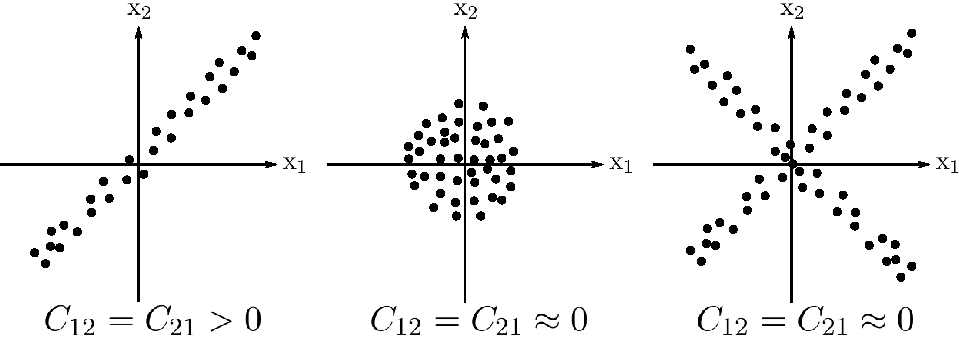
\includegraphics[width=12cm]{section2_fig3}  
\caption{Illustration of data patterns: Note that $C_{ij} = 0$ does
  \underline{not} imply that there are no dependencies between the
  variables. Clearly, $p(\mathrm{x}_1,\mathrm{x}_2) \neq
  p(\mathrm{x}_1)p(\mathrm{x}_2)$ in the third example.}
  \label{fig:correlations}
\end{figure}
\\
First moment of the data projected onto an arbitrary complex feature $\vec{e}_a$:
\begin{equation} \tag{mean}
	\begin{array}{ll}
		m_a 
		& = \frac{1}{p} \sum\limits_{\alpha = 1}^p u_a^{(\alpha)} \\\\
		& = \frac{1}{p} \sum\limits_{\alpha = 1}^p \vec{e}_a^T \cdot
			\vec{x}^{(\alpha)} \\\\
		& = \vec{e}_a^T \cdot \vec{m}
	\end{array}	
\end{equation}
Second moment along this direction:
\begin{equation} \tag{variance}
	\begin{array}{ll}
	\sigma_a^2 
	& = \frac{1}{p} \sum\limits_{\alpha = 1}^p \Big( u_a^{(\alpha)} - m_a
		\Big)^2 \\\\
	& = \frac{1}{p} \sum\limits_{\alpha = 1}^p \Big( \vec{e}_a^T
		\vec{x}^{(\alpha)} - \vec{e}_a^T \vec{m} \Big)^2 \\\\
	& = \frac{1}{p} \sum\limits_{\alpha = 1}^p \bigg\{
		\Big( \vec{e}_a^T \vec{x}^{(\alpha)} \Big)^2
		- 2 \Big( \vec{e}_a^T \vec{x}^{(\alpha)} \Big) \vec{e}_a^T
		\vec{m} + \Big( \vec{e}_a^T \vec{m} \Big)^2
		\bigg\} \\\\
	& \text{with } \vec{e}_a^T \vec{x}^{(\alpha)} = \sum\limits_{i = 1}^N
		\big( \vec{e}_a \big)_i \vec{x}_i^{(\alpha)} \text{ we obtain}
		\\\\
	& = \sum\limits_{i,j = 1}^N \big( \vec{e}_a \big)_i \frac{1}{p}
		\sum\limits_{\alpha = 1}^p \bigg\{ \mathrm{x}_i^{(\alpha)}
			\mathrm{x}_j^{(\alpha)} - \mathrm{x}_i^{(\alpha)}
			m_j - \underbrace{ \mathrm{x}_i^{(\alpha)} m_j }_{
				\substack{ = m_i x_j^{(\alpha)} \\
					\text{change of} \\
					\text{indices}} }
			+ m_i m_j \bigg\} \big( \vec{e}_a \big)_j \\\\
	& = \sum\limits_{i,j = 1}^N \big( \vec{e}_a \big)_i \bigg\{
		\underbrace{ \frac{1}{p} \sum\limits_{\alpha = 1}^p
		\Big( \mathrm{x}_i^{(\alpha)} - m_i \Big) \Big(
		\mathrm{x}_j^{(\alpha)} - m_j \Big) }_{
			= C_{ij} } \bigg\} \big( \vec{e}_a \big)_j
	\end{array}
\end{equation}
\begin{equation}
	\fbox{$ \sigma_a^2 = \vec{e}_a^T \vec{C} \vec{e}_a
	$}
\end{equation}
\textbf{Observation:} The covariance matrix determines the variance of
the data along every possible direction.

% -----------------------------------------------------------------------------

\subsubsection{The Principle of Maximal Variance}
''interesting'' complex features:
\begin{itemize}
	\itR properties of the data which vary most strongly across the data set and might therefore allow to characterize different data points
	\itR direction in feature space along which variance is maximal
		\[ \left. \begin{array}{ll}
			\fbox{$ \sigma_a^2 = \max \big( \vec{e}_a \big) $} \\\\
			\fbox{$ \vec{e}_a^2 = 1 $}
		\end{array} \right. 
		\substack{ 	\text{optimisation} \\
				\text{under constraints} } \]
\end{itemize}
Solution is found using the method of Lagrange multipliers:
\begin{equation}
	\underbrace{ \vec{e}_a^T \vec{C} \vec{e}_a }_{
		\text{objective} }
	- \underbrace{ \lambda }_{ \substack{ 	\text{Lagrange} \\
						\text{multiplier}} }
		\underbrace{ \big( \vec{e}_a^2 - 1 \big) }_{
			\text{constraints} }
	\eqexcl \max
\end{equation}
\begin{itemize}
	\itl family of solutions parametrized by $\lambda$
	\itl $\lambda$ must be chosen such that constraints are fulfilled
\end{itemize}
\begin{equation}
	f(\vec{e}_a) := \sum\limits_{i,j = 1}^N \big( \vec{e}_a \big)_i C_{ij} \big( \vec{e}_a
		\big)_j - \lambda \Bigg\{ \sum\limits_{i = 1}^N \big(
		\vec{e}_a \big)_i^2 - 1 \Bigg\} \eqexcl \max
\end{equation}
\begin{equation}
	\frac{\partial f}{\partial \big( \vec{e}_a \big)_k} \eqexcl 0
	\text{ for all components }k
\end{equation}
\begin{equation}
	\sum\limits_{j = 1}^N C_{kj} \big( \vec{e}_a \big)_j 
		+ \sum\limits_{i = 1}^N \big( \vec{e}_a \big)_i C_{ik}
		- 2 \lambda \big( \vec{e}_a \big)_k \eqexcl 0
\end{equation}
\begin{equation}
	2 \sum\limits_{j = 1}^N C_{kj} \big( \vec{e}_a \big)_j - 2 \lambda
		\big( \vec{e}_a \big)_k \eqexcl 0
		\text{ because } \vec{C} \text{ is symmetric}
\end{equation}
\begin{equation} \tag{eigenvalue problem}
	\fbox{$ \vec{C} \vec{e}_a = \lambda \vec{e}_a $}
\end{equation}
\begin{itemize}
	\itl $\vec{e}_a$ is an eigenvector of $\vec{C}$
	\itl $\vec{e}_a^2 = 1$ can always be fulfilled (through normalization)
	\itl variance $\sigma_a^2 = \vec{e}_a^T \vec{C} \vec{e}_a
		= \lambda \vec{e}_a^2 = \lambda_a$ \\
		eigenvalues: variances of the data along the directions given by
		the eigenvectors
\end{itemize}
\[\fbox{$ \substack{ \text{The eigenvectors of } \vec{C} \text{ with the largest
	(smallest) eigenvalue points} \\ 
	\text{in the direction of the largest (smallest) variance of the data} 
	} $}
\]

% -----------------------------------------------------------------------------

\subsubsection{Principal Components}
Principal component: (normalized) eigenvector $\vec{e}$ of a covariance matrix $\vec{C}$
\\\\
Covariance matrix $\vec{C}$:
\begin{itemize}
  \item real valued
  \item symmetric
  \item positive semidefinite, all eigenvalues must be positive or zero\\
		(they are variances!)
\end{itemize}
\paragraph{Properties of principal components}
\begin{enumerate}[(1)]
\item covariance matrix $\vec{C}$ is real and symmetric (all eigenvalues have to be nonnegative -- $\lambda$s are variances!)
\begin{itemize}
	\itr eigenvectors form an orthonormal basis:
		\begin{equation}
			\vec{e}_i^T \cdot \vec{e}_j = \delta_{ij} 
			\leftarrow \text{ Kronecker-Delta }
			\delta_{ij} = \left\{ \begin{array}{ll}
				1, & i=j \\\\
				0, & \text{else}
			\end{array} \right.
		\end{equation}
	\itr $\vec{C}$ is $N \times N$ matrix $\leadsto N$ eigenvectors
\end{itemize}
\item $\vec{C}$ is diagonal w.r.t. its eigenbasis 
\\\\
\indent let $\vec{M} = \big( \vec{e}_1 \vec{e}_2, \ldots, \vec{e}_N \big)$ then
\begin{equation}
	\vec{M}^T \vec{C} \vec{M} = \widehat{\vec{C}} = 
	\left( \begin{array}{ccccc}
		\lambda_1 \\
		& \lambda_2 & & \text{{\huge{0}}} \\
		& & \ddots \\
		& \text{{\huge{0}}} & & \ddots \\
		& & & & \lambda_N
	\end{array} \right)
	\substack{	\text{transformation into} \\
			\text{the eigenbasis} }
\end{equation}
\begin{itemize}
	\itr principal components are uncorrelated
	\itr transformation into the eigenbasis leads to uncorrelated 
		''complex'' features
\end{itemize}
\item interpretation of principal components w.r.t. variance \slideref{interpretation of PCs}
\begin{equation}
	\begin{array}{ccccccccccc}
		\lambda_1 & > & \lambda_2 & > & \lambda_3 & > 
		& \ldots\ldots & >
		& \lambda_{N-1} & > & \lambda_N \\
		\downarrow && \downarrow && \downarrow 
		&&&& \downarrow && \downarrow \\
		\vec{e}_1 && \vec{e}_2 && \vec{e}_3 
		&&&& \vec{e}_{N-1} && \vec{e}_N
	\end{array}
\end{equation}
\[ \fbox{$ \substack{ \text{direction of} \\ \text{largest variance} } $}
	\longrightarrow \text{?} \longrightarrow 
	\fbox{$ \substack{ \text{direction of} \\ \text{smallest variance} } $}
\]
$\vec{e}_j$ points to the direction of largest variance within the 
	subspace of $\mathbb{R}^N$ spanned by all $\vec{e}_i$ with $i > j$.
      
\item optimal dimensionality reduction: consider the transformation
        of data points into eigenvectors of $\vec{C}$
\begin{equation}
	\vec{x} = \underbrace{ a_1 }_{ \vec{e}_1^T \vec{x} } \vec{e}_1
		+ \underbrace{ a_2 }_{ \vec{e}_2^T \vec{x} } \vec{e}_2
		+ \ldots
		+ \underbrace{ a_N }_{ \vec{e}_N^T \vec{x} } \vec{e}_N
\end{equation}
The projection into the subspace by the $M$ principal components with the
	largest eigenvalues ($M < N$)
\begin{equation}
	\widetilde{\vec{x}} = a_1 \vec{e}_1 + a_2 \vec{e}_2 + \ldots
		+ a_M \vec{e}_M 
\end{equation}
then yields an approximation error:
\begin{equation}
	( \vec{x} - \widetilde{\vec{x}} )^2 = \sum\limits_{j = M+1}^N a_j^2
\end{equation}
\begin{center}
	\fbox{$ \substack{ \text{This reconstruction error is minimal 
				w.r.t. all} \\
		\text{possible projections into } M \text{-dimensional 
		subspaces} } $}
\end{center}
\end{enumerate}
% -----------------------------------------------------------------------------
\subsubsection{Latent factors}
\begin{itemize}
		\item the data may appear high dimensional, but there may only be a small number of features underlying variability
		
		\item dimensionality reduction: projection of the data into a low dimensional subspace which captures the ''essence'' of the data
	
		\item latent factors: remaining PCs with high variance 
	\end{itemize} \slideref{Ex: Eigenfaces} \slideref{Ex: Spiking activity in monkey visual cortex}

% -----------------------------------------------------------------------------

\subsubsection{Summary of \underline{P}rincipal \underline{C}omponent
		\underline{A}nalysis (PCA)}
given observations: $\vec{x}^{(\alpha)}, \alpha = 1, \ldots, p; \vec{x}^{(\alpha)} \in \mathbb{R}^N$

\begin{enumerate}[(1)]
\item normalization to zero mean
\begin{equation}
	\vec{m} = \frac{1}{p} \sum\limits_{\alpha = 1}^p \vec{x}^{(\alpha)}
		\leadsto \widehat{\vec{x}}^{(\alpha)} 
		\leftarrow \vec{x}^{(\alpha)} - \vec{m}
\end{equation}
\item calculation of the covariance matrix $\vec{C}$
\begin{equation}
	C_{ij} = \frac{1}{p} \sum\limits_{\alpha = 1}^p 
		\widehat{\mathrm{x}}_i^{(\alpha)} 
		\widehat{\mathrm{x}}_j^{(\alpha)}
\end{equation}
\item solve the eigenvalue problem
\begin{equation}
	\vec{C} \vec{e} = \lambda \vec{e}
\end{equation}
\end{enumerate}
\textbf{Note:} The eigenvectors of $\vec{C}$ are called \emph{Principal Components}
\\\\
Numerical method: singular value decomposition (see \cite{PressEtAl2007}, chapt. 2.9, Jacobi transformations: chapt. 11.1, reduction and QL: chapt. 11.2-11.3) or simply use a linear algebra package.


\paragraph{Example -- PCA of the Leptograpsus data:} \slideref{projections for Leptograpsus data}
5 dimensions $\rightarrow$ 5 \underline{p}rincipal \underline{c}omponents (PCs)
\[ \left. \begin{array}{ll}
	\text{PC1:} & \text{''size''} \\
	\text{PC2:} & \text{''sex''} \\
	\text{PC3:} & \text{''color/subspecies''}
\end{array} \right\} \substack{ \text{relative importance of elementary} \\
				\text{features can be ''read out'' from} \\
				\text{the feature vectors} }
\]
\begin{itemize}
	\itR example for successful visualization
	\itR example for a successful preprocessing for classification
\end{itemize}
\begin{figure}[h]
  \centering
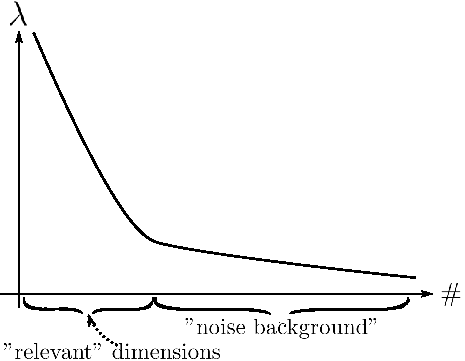
\includegraphics[width=8cm]{section2_fig4}  
  \caption{scree plots (ordering of eigenvalues by size):}
  \label{fig:screePlot}
\end{figure}

\paragraph{Comments:}
\begin{itemize}
\item variance is a scale sensitive measure (e.g.\ using centimeters instead
  of millimeters along one dimension will change all PCs)
	\item max. variance criterion only makes sense if scales are 
		''comparable''
	\item still: PCA constructs uncorrelated features (independent of scale)
	\item PCA is often used for ''whitening'': scale variance along all
		directions to one
\end{itemize}

% -----------------------------------------------------------------------------

\newpage 						% for visual reasons
\subsection{Hebbian Learning for Linear Neurons}
\begin{figure}[h]
  \centering
\[ \begin{array}{ll}
	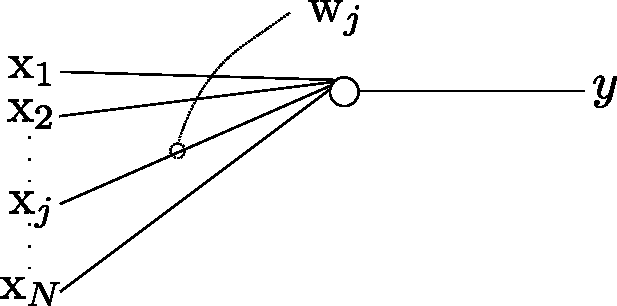
\includegraphics[width=6cm]{section2_fig5}
	& y = \vec{w}^T \vec{x}
\end{array} \]
  \caption{Linear connectionist neuron}
  \label{fig:linearConnectionistNeuron}
\end{figure}
observations: $\vec{x}^{(\alpha)}, \alpha = 1, \ldots, p, \vec{x}^{(\alpha)} \in \mathbb{R}^N$

\begin{algorithm}[h]
  \DontPrintSemicolon
  initialization of weights (e.g.\ to small numbers)\;
  choose learning rate $\varepsilon$\;
  \Begin(loop){
    Choose an observation  $\vec{x}^{(\alpha)}$\;
    Change weights according to:\;
    \begin{equation}
      \underbrace{ \Delta \mathrm{w}_j = \varepsilon 
        y_{ \big( \vec{x}^{(\alpha)}; \vec{w} \big) }
        \vec{x}^{(\alpha)} }_{
        \substack{\text{weights increase (decrease) if input}\\
          \text{and output are correlated (anticorrelated)}}}
    \end{equation}    
  }
  \label{alg:HebbianLearning}
  \caption{Hebbian (correlation-based) learning for linear neurons}
\end{algorithm}

\paragraph{Proposition:} Applied to linear neurons, Hebbs rule extracts the PC with the largest Eigenvalue.

\paragraph{Proof:}
small learning steps $\leadsto$ average over all patterns
\begin{equation}
	\begin{array}{ll}
		\Delta \mathrm{w}_j 
		& \approx \frac{\varepsilon}{p} \sum\limits_{\alpha = 1}^p 
			y_{\big( \vec{x}^{(\alpha)};
			\vec{w} \big) } \mathrm{x}_j^{(\alpha)} \\\\
		& = \frac{\varepsilon}{p} \sum\limits_{\alpha = 1}^p
			\sum\limits_{k = 1}^N \mathrm{w}_k
			\mathrm{x}_k^{(\alpha)} \mathrm{x}_j^{(\alpha)} \\\\
		& = \varepsilon \sum\limits_{k = 1}^N \mathrm{w}_k C_{kj}
	\end{array}
\end{equation}
\begin{equation}
	\Delta \vec{w} = \varepsilon \vec{C} \vec{w} \leadsto 
		\substack{ 	\text{''analysis'' of the} \\
				\text{covariance matrix} }
\end{equation}
transformation into the eigenbasis of $\vec{C}$
\\\\
let: $\lambda_1 > \lambda_2 > \ldots > \lambda_N \leftarrow$ eigenvalues
\begin{equation}
	\vec{w} = a_1 \vec{e}_1 + a_2 \vec{e}_2 + \ldots + a_N \vec{e}_N 
		\leftarrow \text{ corresponding eigenvectors}
\end{equation}
then:
\begin{equation}
	\Delta a_j = \varepsilon \lambda_j a_j
\end{equation}

\begin{figure}[h]
  \centering
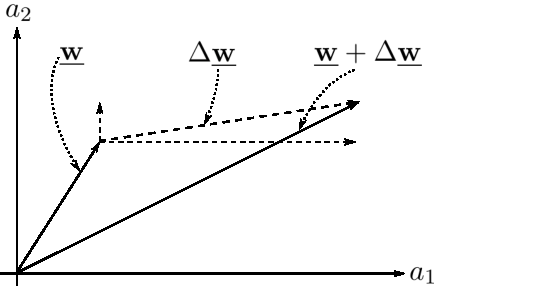
\includegraphics[width=10cm]{section2_fig6}  
  \caption{Learning via Ojas rule}
  \label{fig:learningOjasRule}
\end{figure}



\begin{itemize}
	\itr $|\vec{w}| \rightarrow \infty$
	\itr $\vec{e}_{\mathrm{w}} = \frac{\vec{w}}{|\vec{w}|}$ converges to
		$\vec{e}_1$ (eigenvector with the largest eigenvectors)
\end{itemize}

Note: in the Haykin book a proof for the more general stochastic algorithm can be 
found showing the generality of the statement.

\paragraph{Neurobiological implications} 
\begin{itemize}
\item receptive fields and coding
\item adaptive tracking of the direction of largest variance: ''on-line'' PCA
\end{itemize}
%
\emph{Problem:} $\|w\| \to \infty$ \ra requires some form of normalization
\\\\
\emph{Solution:} Normalization via Oja's rule
\begin{equation}
	\Delta \mathrm{w}_j = \varepsilon y_{ \big( \vec{x}^{(\alpha)}; \vec{w}
		\big) } \bigg\{ 
			\underbrace{ \mathrm{x}_j^{(\alpha)} }_{
				\substack{	\text{Hebbian} \\
						\text{learning} }}
			- \underbrace{ y_{ \big( \vec{x}^{(\alpha)}; \vec{w}
				\big) } \mathrm{w}_j }_{ 
				\substack{	\text{decay} \\
						\text{term} }}
			\bigg\}
\end{equation}
Oja's rule converges to the unit vector which points into the direction of the
largest variance 
\\\\
{\it proof: supplementary material}

\paragraph{Hebbian PCA (generalized Hebbian algorithm):}
\begin{center}
		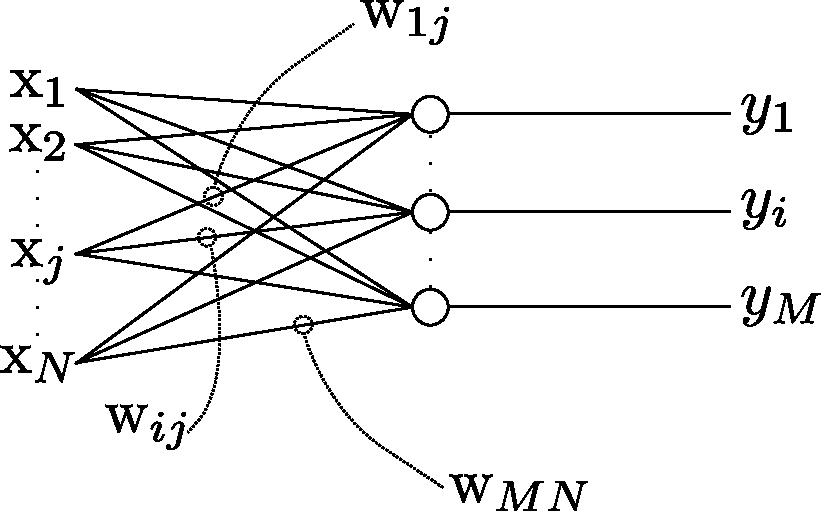
\includegraphics[width=6cm]{section2_fig5_b}
\end{center}
	$\text{M linear neurons: } y_i = \vec{w}_i^T \vec{x} = \sum_{j=1}^{N} \mathrm{w}_{ij} \mathrm{x}_j $, $i=1, \dots, M$\\
	observations: $\vec{x}^{(\alpha)},\quad \alpha = 1, \ldots, p,\quad \vec{x}^{(\alpha)} \in \mathbb{R}^N$ \\ 
	\vspace{5mm}
	The (feedforward) neural network extracts the $M$ PCs with the largest eigenvalues\\
	\begin{itemize}
		\itl online-PCA for data with time-varying statistics
	\end{itemize} 

\paragraph{Extended learning (Sanger's rule)}
\begin{equation*}
			\Delta \mathrm{w}_{ij} = \varepsilon y_i \bigg\{ \underbrace{\mathrm{x}_j}_{\text{Hebbian rule}} - \underbrace{\sum_{k=1}^{i} \mathrm{w}_{kj} y_k}_{\substack{\sum_{k=1}^{i-1} \mathrm{w}_{kj} y_k  \text{ is added to Oja's rule}}} \bigg\}
		\end{equation*}

\begin{itemize}
		\itl weights converge to the $M$ eigenvectors with the largest eigenvalues \\ \vspace{0.2cm}
\begin{tabular}{ccc}
			$\vec{w}_1$ & $\rightarrow$ & $\vec{e}_1$ \\ 
			$\vec{w}_2$ & $\rightarrow$ & $\vec{e}_2$ \\ 
						& $\vdots$ &  \\ 
			$\vec{w}_M$ & $\rightarrow$ & $\vec{e}_M$  
\end{tabular}
		\vspace{0.2cm}
		\itl $y_i = \vec{e}_i^T \vec{x} =: a_i$ after learning
\end{itemize}

\paragraph{Learning: Oja's rule \& Gram-Schmidt orthonormalization}\mbox{}\\
	Sanger's rule: $\Delta \mathrm{w}_{ij} = \varepsilon y_i \bigg\{ \mathrm{x}_j - \sum_{k=1}^{i} \mathrm{w}_{kj} y_k \bigg\}$
	\begin{itemize}
		\item Define $\hat{\mathrm{x}}_j^{(i)} := \mathrm{x}_j - \sum_{k=1}^{i-1} \mathrm{w}_{kj} y_k$
		\item Then $\Delta \mathrm{w}_{ij} = \varepsilon y_i \left\{ \hat{\mathrm{x}}_j^{(i)} - y_j \mathrm{w}_{ij} \right\} 		  					\longrightarrow$ Oja's rule with modified input
	\end{itemize}
	
\textbf{Case $i=1$:}:\\
\begin{tabular}{lll}
			$\hat{\mathrm{x}}_j^{(1)} = \mathrm{x}_j$ & $\leadsto$ & original form of Oja's rule \\
								                      & $\leadsto$ & $\vec{w}_1$ converges to eigenvector $\pm \vec{e}_1$
\end{tabular}\\
\vspace{0.3cm}
\begin{wrapfigure}{r}{0.5\textwidth}
  \begin{center}
    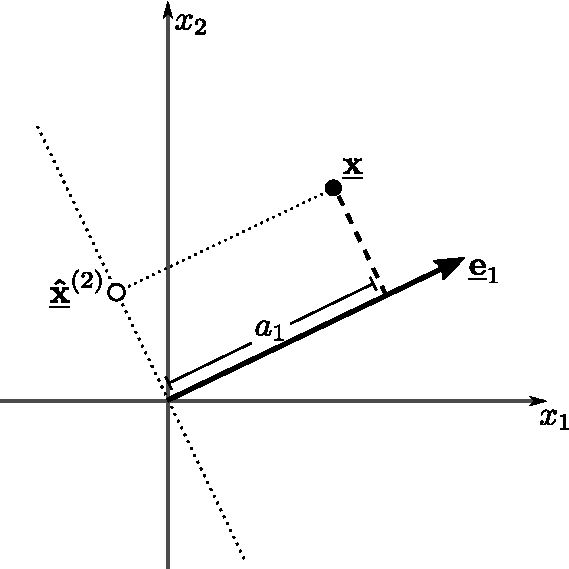
\includegraphics[width=0.4\textwidth]{section1_fig7}
  \end{center}
  \caption{novelty orthonormalization}
\end{wrapfigure}
\textbf{Case $i=2$:}\\
		$\hat{\mathrm{x}}_j^{(2)} = \mathrm{x}_j - \mathrm{w}_{1j} y_1$ \\
		$\vec{w}_1 = \vec{e}_1 \rightarrow y_1 = \vec{x}^T \vec{e}_1 =: a_1$ \\ \& $\hat{\mathrm{x}}_j^{(2)} = \mathrm{x}_j - \left( \vec{e}_1 \right)_j a_1$\\
\begin{itemize}
	\itr $\hat{\vec{x}}^{(2)}$ is the projection of $\vec{x}$ onto subspace orthogonal to $\vec{e}_1$:
	\begin{itemize}
	\itr $\vec{w}_2$ converges to $\pm \vec{e}_2$ by Oja's rule since $\vec{e}_2$ is the direction of largest variance in that subspace
	\end{itemize}
\end{itemize}
\vspace{0.7cm}
\textbf{Case $i=3$:}\\
$\hat{\mathrm{x}}_j^{(3)} = \mathrm{x}_j - \mathrm{w}_{1j} y_1 - \mathrm{w}_{2j} y_2$ \\ 
$$\vec{w}_1 = \vec{e}_1 \hspace{0.1cm} \& \hspace{0.1cm} \vec{w}_2 = \vec{e}_2 \rightarrow y_1 = a_1, \hspace{0.2cm} y_2 = \vec{x}^T \hspace{0.2cm} \vec{e}_2 =: a_2\\ 
\hspace{0.1cm} \& \hspace{0.1cm}\hat{\mathrm{x}}_j^{(3)} = \mathrm{x}_j - a_1 \left( \vec{e}_1 \right)_j - a_2 \left( \vec{e}_2 \right)_j$$
\begin{itemize}
\itr $\hat{\vec{x}}^{(3)}$ is the projection of $\vec{x}$ onto subspace orthogonal to $\operatorname{span}\left\{ \vec{e}_1, \vec{e}_2 \right\}$
\itr $\vec{w}_3$ converges to $\pm \vec{e}_3$ by Oja's rule\\
\end{itemize}
\vspace{0.1cm}
\textbf{Case $i=M$:}\\
$\hat{\mathrm{x}}_j^{(M)} = \mathrm{x}_j - \sum_{k=1}^{M-1} \mathrm{w}_{kj} y_k$ \\
$\vec{w}_k = \vec{e}_k \text{ for }k=1,\dots, M-1 \rightarrow y_k = \vec{x}^T \vec{e}_k =: a_k$ \\ 
\& $\hat{\mathrm{x}}_j^{(M)} = \mathrm{x}_j - \sum_{k=1}^{M-1} a_k \left( \vec{e}_k \right)_j$ 

\begin{itemize}
\itr $\hat{\vec{x}}^{(M)}$ is the proj. of $\vec{x}$ onto subspace orthogonal to $\operatorname{span}\left\{ \vec{e}_1, \hdots, \vec{e}_{M-1} \right\}$ 
\itr $\vec{w}_M$ converges to $\pm \vec{e}_M$ by Oja's rule
\end{itemize}

\paragraph{Summary of Hebbian learning: }\mbox{}\\
\textbf{I. Hebbian learning without constraint}\\
		\begin{equation*}
			\underbrace{\Delta \vec{w} = \varepsilon y \vec{x}}_{\text{Hebb's rule}} \leadsto \lim\limits_{t \rightarrow \infty} \vec{w} || \vec{e}_1 \text{ (orthogonal)}
		\end{equation*}
$\leadsto$ weights converge to direction of largest variance in the data\\
$\leadsto$ but: $|\vec{w}| \rightarrow \infty$ for $t \rightarrow \infty$

\textbf{II. Hebbian learning with normalization}\\
		\begin{equation*}
			\underbrace{\Delta \vec{w} = \varepsilon y \left( \vec{x} - y \vec{w} \right)}_{\text{Oja's rule}} \leadsto \lim\limits_{t \rightarrow \infty} \vec{w} \in \left\{ +\vec{e}_1, -\vec{e}_1 \right\}
		\end{equation*}
$\leadsto$ weights remain finite: $|\vec{w}| = 1$

\textbf{III. Hebbian PCA with $M$ neurons and normalization}\\
		\begin{equation*}
			\underbrace{\Delta \mathrm{w}_{ij} = \varepsilon y_i \left\{ \mathrm{x}_j - \sum_{k=1}^{i} \mathrm{w}_{kj} y_k \right\} }_{\text{Sanger's rule}} \leadsto \lim\limits_{t \rightarrow \infty} \vec{w}_i \in \left\{ +\vec{e}_i, -\vec{e}_i \right\}, i=1, \hdots, M
		\end{equation*}
		$\leadsto$ combination of Oja's rule \& Gram-Schmidt-orthonormalization




% -----------------------------------------------------------------------------

\newpage 						% for visual reasons
\subsection{Kernel Principal Component Analysis}
Kernel PCA extends the linear dimensionality reduction approach of PCA to extract nonlinear structure. 
% -----------------------------------------------------------------------------
\subsubsection{Non-linear Manifolds}
\begin{figure}[h]
  \centering
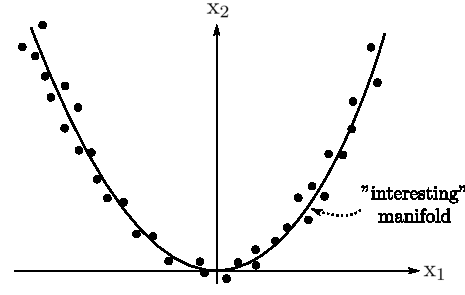
\includegraphics[width=8cm]{section2_fig7}  
  \caption{Example of a nonlinear dependency}
  \label{fig:nonlinearDependency}
\end{figure}
%
Consider the data represented in the original space:
\begin{itemize}
  \item standard PCA: two directions with high variance
  \item ''interesting'' feature is a non-linear combination of
    elementary features \itl this dependency is not properly extracted
    by standard PCA
\end{itemize}

\begin{figure}[h]
  \centering
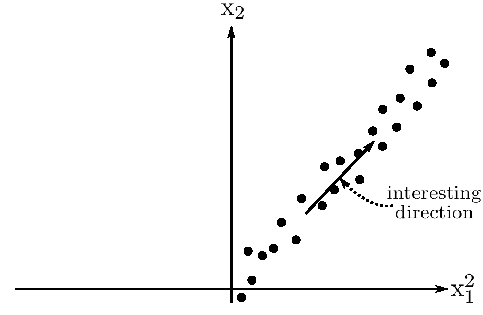
\includegraphics[width=8cm]{section2_fig8}  
  \caption{Nonlinear dependency becomes linear in transformed space}
  \label{fig:transformedDependency}
\end{figure}


Idea: analyse data in \emph{transformed} (feature) space:
\begin{itemize}
	\itl standard PCA: one direction of high variance
	\itl ''interesting'' feature will be discovered
\end{itemize}
\textbf{Agenda:} non-linear preprocessing, then application of a
standard linear method $\Rightarrow$ non-linear analysis method,
i.e.\ given a set of observations: $\vec{x}^{(\alpha)}, \alpha = 1,
\ldots, p; \vec{x}^{(\alpha)} \in \mathbb{R}^N$
\begin{enumerate}[(1)]
\item transformation into an ''appropriate'' feature space
\begin{equation}
	\vec{\phi}: \vec{x} \rightarrow \vec{\phi}_{(\vec{x})}
\end{equation}
\item apply \emph{linear} analysis method on $\vec{\phi}_{(\vec{x})}$
\end{enumerate}
\textbf{Problem:} Some feature spaces may be extremely high-dimensional

\begin{figure}[h]
  \centering
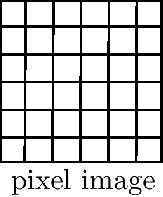
\includegraphics[width=3cm]{section2_fig9}  
  \caption{Pixel image as a high dimensional patterns}
  \label{fig:pixelImage}
\end{figure}


\begin{itemize}
  \itl interesting structure is hidden in correlations between pixel 
  values
  \itl 'interesting'' feature space: space spanned by all 
  $d^{\mathrm{th}}$-order monomials
  \begin{equation}
    \text{e.g. } d = 2: 
    \mathrm{x}_1^2, \mathrm{x}_1 \mathrm{x}_2, 
    \mathrm{x}_2^2, \mathrm{x}_1 \mathrm{x}_3, 
    \mathrm{x}_2 \mathrm{x}_3, \mathrm{x}_3^2, \ldots
  \end{equation}
  \itl number of dimensions
  \begin{equation}
    \frac{ (N+d-1)! }{ d!(N-1)! } 
    = O_{ \big( N^d \big) }
  \end{equation}
\end{itemize}
Are there methods which work in the original space $\mathbb{R}^N$? \\
Yes! Use the kernel trick ({\it see also MI I, chapter 2.2.4}).

% -----------------------------------------------------------------------------
\subsubsection{Reformulation of PCA using only Scalar Products}
Observations: $\vec{x}^{(\alpha)}, \alpha = 1, \ldots, p; \vec{x}^{(\alpha)} \in \mathbb{R}^N$
\\\\
Simplifying assumptions:
\begin{equation}
	\frac{1}{p} \sum\limits_{\alpha = 1}^p \vec{x}^{(\alpha)} = \vec{0}
		\leadsto \text{ zero mean data}
\end{equation}
Correlation matrix $\vec{C}$:
\begin{equation}
	C_{ij} = \frac{1}{p} \sum\limits_{\alpha = 1}^p \mathrm{x}_i^{(\alpha)}
		\mathrm{x}_j^{(\alpha)} 
		\Rightarrow \vec{C} = \frac{1}{p} \sum\limits_{\alpha = 1}^p
			\vec{x}^{(\alpha)} \Big( \vec{x}^{(\alpha)} \Big)^T
\end{equation}
PCA requires a solution of the eigenvalue problem:
\begin{equation}
	\vec{C} \vec{e}_k = \lambda_k \vec{e}_k
\end{equation}
Expansion of the eigenvectors into data points (linear combination, not necessarily unique):
\begin{equation}
	\underbrace{ \vec{e}_k = \sum\limits_{\beta = 1}^p a_k^{(\beta)} 
		\vec{x}^{(\beta)}
	}_{ \substack{	\text{always possible, because principal 
					components}\\
				\text{lie in the subspace of the data} } }
\end{equation}
Insertion into the eigenvalue equation leads to:
\begin{equation}
	\frac{1}{p} \sum\limits_{\alpha, \beta = 1}^p a_k^{(\beta)}
	\bigg[ \Big( \vec{x}^{(\alpha)} \Big)^T \vec{x}^{(\beta)} \bigg]
	\vec{x}^{(\alpha)} = \lambda_k \sum\limits_{\beta = 1}^p
	a_k^{(\beta)} \vec{x}^{(\beta)}
\end{equation}
%Projections onto the directions given by data points $\Big( \vec{x}^{(\gamma)} \Big)^T$:
Multiplying with data points $\Big( \vec{x}^{(\gamma)} \Big)^T$, $\gamma = 1,\dots,p$:
\begin{equation}
	\frac{1}{p} \sum\limits_{\alpha, \beta = 1}^p a_k^{(\beta)}
	\bigg[ \Big( \vec{x}^{(\alpha)} \Big)^T \vec{x}^{(\beta)} \bigg]
	\bigg[ \Big( \vec{x}^{(\gamma)} \Big)^T \vec{x}^{(\alpha)} \bigg]
	= \lambda_k \sum\limits_{\beta = 1}^p a_k^{(\beta)} 
	\bigg[ \Big( \vec{x}^{(\gamma)} \Big)^T \vec{x}^{(\beta)} \bigg]
\end{equation}
Formulation of the eigenvalue problem in terms of scalar products:
\begin{equation}
	K_{\alpha \beta} \coloneqq \Big( \vec{x}^{(\alpha)} \Big)^T 
		\vec{x}^{(\beta)}
\end{equation}
in matrix notation (generalized eigenvalue problem):
\begin{equation}
	\vec{K}^2 \vec{a}_k = p \lambda_k \vec{K} \vec{a}_k
\end{equation}
\textbf{Remark:} $\vec{K}$ is a positive semidefinite matrix! Why? Because
for an arbitrary vector $\vec{y}$:
\begin{equation}
	\begin{array}{ll}
	\vec{y}^T \vec{K} \vec{y} 
	& = \sum\limits_{\alpha, \beta = 1}^p
		y^{(\alpha)} \Big( \vec{x}^{(\alpha)} \Big)^T
		\vec{x}^{(\beta)} y^{(\beta)} \\\\
	& = \Bigg( \sum\limits_{\alpha = 1}^p y^{(\alpha)} \vec{x}^{(\alpha)}
		\Bigg)^2 \\\\
	& \geq 0
	\end{array}
\end{equation}

Positive semidefiniteness of $\vec{K}$
means,
it has only non-negative eigenvalues (but potentially 0) 
\ra
% can be inverted \ra multiply by $K^{-1}$ from the left. \ra 
solutions
of the following transformed (standard eigenvalue) problem differ only by components corresponding to
% orthogonal to the
uninteresting directions with zero eigenvalues
% solution space 
(see e.g.\ \cite{Bishop2006}).
\\\\
Transformed eigenvalue problem:
\begin{equation}
	\fbox{$ \vec{K} \vec{a}_k = p \lambda_k \vec{a}_k $}
\end{equation}
\[ \begin{array}{ll}
	\vec{K}: & \text{matrix of scalar products between data points} \\\\
	\lambda_k: & \text{variance along principal component } \vec{a}_k \\\\
	\vec{a}_k: & \text{principal component, represented in the - may be 
		autocomplete -} \\
	&	\text{basis } \Big\{ \vec{x}^{(\alpha)} \Big\}, 
		\alpha = 1, \ldots, p
\end{array} \]
Normalization of principal components
\begin{equation}
	\begin{array}{ll}
		\vec{e}_k^2 
		& = \sum\limits_{\alpha, \beta = 1}^p a_k^{(\alpha)} 
			\Big( \vec{x}^{(\alpha)} \Big)^T \vec{x}^{(\beta)}
			a_k^{(\beta)} \\\\
		& = \vec{a}_k^T \vec{K} \vec{a}_k  \\\\
		& = \lambda_k \vec{a}_k^2 p\\\\
		& \eqexcl 1
	\end{array}
\end{equation}
\begin{equation}
	\fbox{$ \vec{a}_k^{\mathrm{norm.}} = 
			\frac{1}{\sqrt{p} \sqrt{\lambda_k} |\vec{a_k}|} 
			\vec{a}_k $}
\end{equation}
Projection $u_k$ of a new data vector $\vec{x}$ onto the principal components
\begin{equation}
	\begin{array}{ll}
	u_k
	& = \vec{e}_k^T \cdot \vec{x} \\\\
	& = \sum\limits_{\beta = 1}^p a_k^{(\beta)} 
		\underbrace{ \bigg[ \Big( \vec{x}^{(\beta)} \Big)^T 
				\cdot \vec{x} \bigg] }_{
					\text{scalar product} }
	\end{array}
\end{equation}
\textbf{Note:} This formulation of PCA is exclusively in terms of scalar products
\\\\
% -----------------------------------------------------------------------------

\subsubsection{The Kernel Trick}
\textbf{Idea:} perform PCA in a suitable feature space
\begin{equation}
	\vec{\phi}: \vec{x} \xrightarrow{\text{ {\tiny non-linear 
		transformation}}} \vec{\phi}_{(\vec{x})}
\end{equation}
\textbf{Kernel trick:}
\begin{itemize}
	\itR avoid direct transformation $\vec{\phi}$
	\itR replace all scalar products by ''kernel functions''
		\begin{equation}
			\vec{\phi}_{(\vec{x})}^T
			\vec{\phi}_{(\vec{x}')} \longleftrightarrow 
			k_{(\vec{x}, \vec{x}')}
		\end{equation}
\end{itemize}

\paragraph{Mercer's theorem:} 
every positive definite kernel $k$ corresponds to a scalar product in 
some metric feature space\footnote{for details see MI I, chapt. 2.2.4} 
\\\\
{\bf Typical kernel functions}
\[ \begin{array}{ll}
	k_{(\vec{x},\vec{x}')} = \big( \vec{x}^T \vec{x}' + 1 \big)^d
	& \substack{	\text{polynomial kernel of degree } d \\
			\text{{\it image processing (pixel correlation)}} } \\\\
	k_{(\vec{x},\vec{x}')} = \exp \bigg\{ -\frac{ \big( \vec{x} - \vec{x}' 
					\big)^2 }{ 2 \sigma^2 } \bigg\}
	& \substack{ 	\text{RBF-kernel with range } \sigma \\
			\text{{\it infinite dimensional feature space}} } \\\\
	k_{(\vec{x},\vec{x}')} = \tanh \big\{ K \vec{x}^T \vec{x}' + \theta
					\big\}
	& \substack{ 	\text{neural network kernel with parameters } K 
				\text{ and } \theta \\
			\text{{\it not necessarily positive definite}} } \\\\
	k_{(\vec{x},\vec{x}')} = \frac{1}{ |\vec{x} - \vec{x}' + \varepsilon
						|^N }
	& \substack{	\text{Plummer kernel with parameter } \varepsilon \\
			\text{{\it scale invariant kernel}} }
\end{array} \]
\textbf{Note:} no need to explicitly project into feature space -- if
an algorithm can be formulated solely in terms of scalar products, a
non-linear version of it can be derived via this approach. 
\begin{itemize}
	\itl {\it cf. support vector machines (MI I)}
	\itl Fisher discriminant analysis, Canonical Correlation Analysis
	\itl K-means clustering \& self-organizing maps (MI II)
\end{itemize}

\noindent \textbf{Problem: } derivation assumes zero mean -- but
normalization to zero mean in original space does not guarantee normalization in
feature space
\begin{equation}
        \frac{1}{p} \sum\limits_{\alpha = 1}^p \vec{x}^{(\alpha)} \eqexcl 0
        \nrightarrow \frac{1}{p} \sum\limits_{\alpha = 1}^p 
                \vec{\phi}_{\big( \vec{x}^{(\alpha)} \big)} = \vec{0}
\end{equation}
\textbf{Solution:} calculation of ''centered'' kernel matrix elements 
\\\\
data points $\vec{x}^{(\alpha)}$: ''training'' data: $\alpha \in \{1, \ldots, p\}$; new (test) data: $\alpha > p$
\begin{equation}
        \underbrace{ \vec{\phi}_{\big( \vec{x}^{(\alpha)} \big)} }_{
                \substack{      \text{''centered''} \\
                                \text{feature vectors}} }
        = \widetilde{\vec{\phi}}_{\big( \vec{x}^{(\alpha)} \big)}
                - \frac{1}{p} \sum\limits_{\gamma = 1}^p 
                \underbrace{ \widetilde{\vec{\phi}}_{\big( \vec{x}^{(\gamma)} 
                                \big)} }_{
                        \substack{      \text{uncentered} \\
                                        \text{feature vectors}} }
\end{equation}
\begin{equation}
        \begin{array}{lll}
        K_{\alpha \beta}
        & = & \vec{\phi}_{\big( \vec{x}^{(\alpha)} \big)}^T
                \cdot \vec{\phi}_{\big( \vec{x}^{(\beta)} \big)}
                \\\\
        & = & \bigg( \widetilde{\vec{\phi}}_{\big( \vec{x}^{(\alpha)} \big)}^T
                - \frac{1}{p} \sum\limits_{\gamma = 1}^p 
                \widetilde{\vec{\phi}}_{\big( \vec{x}^{(\gamma)} \big)}^T
                \bigg) \bigg(\widetilde{\vec{\phi}}_{\big( \vec{x}^{(\beta)} 
                \big)} - \frac{1}{p} \sum\limits_{\delta = 1}^p 
                \widetilde{\vec{\phi}}_{\big( \vec{x}^{(\delta)} \big)} \bigg)
                \\\\
        & = & \widetilde{\vec{\phi}}_{\big( \vec{x}^{(\alpha)} \big)}^T
                \widetilde{\vec{\phi}}_{\big( \vec{x}^{(\beta)} \big)}
                - \frac{1}{p} \sum\limits_{\gamma = 1}^p 
                \widetilde{\vec{\phi}}_{\big( \vec{x}^{(\gamma)} \big)}^T
                \widetilde{\vec{\phi}}_{\big( \vec{x}^{(\beta)} \big)}
                \\\\
        && - \frac{1}{p} \sum\limits_{\delta = 1}^p 
                \widetilde{\vec{\phi}}_{\big( \vec{x}^{(\alpha)} \big)}^T
                \widetilde{\vec{\phi}}_{\big( \vec{x}^{(\delta)} \big)}
                + \frac{1}{p^2} \sum\limits_{\delta = 1}^p 
                \widetilde{\vec{\phi}}_{\big( \vec{x}^{(\gamma)} \big)}^T
                \widetilde{\vec{\phi}}_{\big( \vec{x}^{(\delta)} \big)}
                \\\\
        & = & \widetilde{K}_{\alpha \beta} - \frac{1}{p} 
                \sum\limits_{\gamma = 1}^p \widetilde{K}_{\gamma \beta}
                -\frac{1}{p} \sum\limits_{\gamma = 1}^p 
                \widetilde{K}_{\alpha \gamma} + \frac{1}{p^2} 
                \sum\limits_{\gamma, \delta} \widetilde{K}_{\gamma \delta}
        \end{array}
\end{equation}



% -----------------------------------------------------------------------------

\subsubsection{Summary of the Kernel-PCA Method}
\begin{enumerate}[(1)]
\item calculate the un-normalized kernel matrix $\widetilde{\vec{K}}$
\begin{equation}
	\widetilde{K}_{\alpha \beta} = \underbrace{ k_{\big( \vec{x}^{(\alpha)},
			\vec{x}^{(\beta)} \big)} }_{
				\substack{ 	\text{kernel} \\
						\text{function}} }
\end{equation}
\item normalize to zero mean
\begin{equation}
	K_{\alpha \beta} = \widetilde{K}_{\alpha \beta} - \frac{1}{p} 
		\sum\limits_{\gamma = 1}^p \widetilde{K}_{\gamma \beta}
		-\frac{1}{p} \sum\limits_{\gamma = 1}^p 
		\widetilde{K}_{\alpha \gamma} + \frac{1}{p^2} 
		\sum\limits_{\gamma, \delta} \widetilde{K}_{\gamma \delta}
\end{equation}
\item solve the eigenvalue problem
\begin{equation}
	\vec{K} \widetilde{\vec{a}}_k = p \lambda_k \widetilde{\vec{a}}_k
\end{equation}
\item normalize eigenvectors to unit length (in feature space)
\begin{equation}
	\vec{a}_k = \frac{1}{\sqrt{p \lambda_k} \, ||\widetilde{\vec{a}}_k||} 
			\widetilde{\vec{a}}_k
\end{equation}
\item calculate projections of data points $\vec{x}^{(\alpha)}$ onto eigenvectors
\begin{equation}
	u_k(\vec{x}^{(\alpha)}) = \sum\limits_{\beta = 1}^p a_k^{(\beta)} 
		K_{\beta \alpha} \leftarrow 
			\substack{	\text{use normalized} \\
					\text{matrix element!}}
\end{equation}
\end{enumerate}

More generally, for arbitrary $\vec{x}$ the projection is computed as:

\begin{align*}
	u_{k}\left (\vec{x} \right ) 
	= & \sum\limits_{\beta = 1}^p a_k^{(\beta)} \vec{\phi}_{\left(\vec{x}^{(\beta)}\right)}^T 
	    \vec{\phi}_{(\vec{x})}	\qquad \leftarrow \text{\scriptsize centered feature vectors} \\
	=  & \sum\limits_{\beta = 1}^p a_k^{(\beta)} 
	    \Big ( \Big [ \widetilde{\vec{\phi}}_{\left(\vec{x}^{(\beta)}\right)}
			  - \frac{1}{p} \sum\limits_{\gamma=1}^p 
				  \widetilde{\vec{\phi}}_{\left(\vec{x}^{(\gamma)}\right)} \Big ]^T 
		   \Big [ \widetilde{\vec{\phi}}_{\left(\vec{x}\right)} 
			  - \frac{1}{p} \sum\limits_{\delta=1}^p 
			      \widetilde{\vec{\phi}}_{\left(\vec{x}^{(\delta)}\right)} \Big ]
	    \Big ) \\
	= &  \sum\limits_{\beta = 1}^p a_k^{(\beta)} 
	    \Big (
		k(\vec{x}^{(\beta)}, \vec{x})
		- \frac{1}{p} \sum\limits_{\delta=1}^p \widetilde K_{\beta \delta} 
		- \frac{1}{p} \sum\limits_{\gamma=1}^p k(\vec{x}^{(\gamma)}, \vec{x})
		+ \frac{1}{p^2} \sum\limits_{\gamma,\delta=1}^p \widetilde K_{\gamma \delta}
	    \Big )
\end{align*}


\paragraph{Comments:}
\begin{itemize}
\item kernel-PCA $\corresponds$ PCA in feature space
  \begin{itemize}
    \itr ''principal components'' are uncorrelated
    \itr $\lambda_k$: variance of the data along principal component
    $k$ ( in feature space)
    \itr mean-squared approximation error (in feature space) in representing the 
    observations by components with largest eigenvalues
    is minimal
  \end{itemize}
\item for KPCA, number of principal components can exceed number of
  dimensions in the original space
  \item reconstruction is harder as in linear PCA: no explicit data space representation of the 
  principal component subspace
  \begin{itemize}
   \item typically only projection coefficients $u_k(\vec{x})$ are used
   \item data space is mapped to low-dim. manifold in feature space
   \item for general feature vectors: no pre-image in data space
   \item but: approximative pre-images can be computed (application: denoising)
  \end{itemize}
  \item Kernel PCA can be used for feature extraction, e.g., to solve classification problems in feature space
  \item Optimal kernel parameters ($\sigma$, $d$, etc.) depend on data \& task (selection via cross-validation possible for classification tasks but in general no measure-of-goodness of the PC projections available)
  \item Custom kernels can be used (any positive definite kernel matrix)
\item expansion of principal components into data points is 
  \underline{not} sparse
    $\leadsto$ high computational burden when calculating projections
    \\\\
    \emph{possible solution:} approximate principal components using expansions with less data
    vectors $q < p$:
    \begin{equation*}
      \begin{array}{ll}
        \vec{e}_k = \sum\limits_{\beta = 1}^p a_k^{(\beta)}
        \vec{\phi}_{\big( \vec{x}^{(\beta)} \big)}
        & \text{principal (normalized) components } k
        \\\\
        \widehat{\vec{e}}_k = \sum\limits_{\gamma = 1}^q
        \widehat{a}_k^{(\gamma)} 
        \vec{\phi}_{ \underbrace{ \big( 
            \vec{z}^{(\gamma)} \big) }_{
%             \substack{ 	\text{new data} \\
%               \text{pt. order, } \\ }
          }}
        & \text{approximation by $q$ data points \big(in new order, $\vec z^{(\gamma)} = \vec x^{(i_\gamma)}$\big)}
      \end{array}
    \end{equation*}
    quadratic error  $\varphi$:
    \begin{equation*}
      \begin{array}{ll}
        \varphi
        & = \big( \vec{e}_k - \widehat{\vec{e}}_k \big)^2
        \\\\
        & = \underbrace{ |\vec{e}_k|^2 }_{= 1} 
        + | \widehat{\vec{e}}_k |^2 - 2\vec{e}_k^T
        \widehat{\vec{e}}_k
        \\\\
        & = 1 + \sum\limits_{\gamma, \delta = 1}^q 
        \widehat{a}_k^{(\gamma)} 
        \widehat{a}_k^{(\delta)} k_{\big( 
          \vec{z}^{(\gamma)}, \vec{z}^{(\delta)}
          \big)}
        -2 \sum\limits_{\beta = 1}^p 
        \sum\limits_{\gamma = 1}^q 
        a_k^{(\beta)} \widehat{a}_k^{(\gamma)}
        k_{\big( \vec{x}^{(\beta)}, \vec{z}^{(\gamma)}
          \big)}
      \end{array}
    \end{equation*}
    choose $\widehat{a}_k^{(\gamma)}$ and $\vec{z}^{(\gamma)}$ such
    that
    \begin{equation*}
      \varphi \eqexcl \min
    \end{equation*}
    e.g.\ using gradient-based methods

  \item kernel matrices may be very large
  \begin{itemize}
    \itr only eigenvectors to the largest eigenvalues are
    of interest
    \itr use specialized routines (\cite{PressEtAl2007} chapt. 11.5 - 11.7)
  \end{itemize}
  \slideref{toy example (Schölkopf et al., MPI Biol. Cybern.
    Technical Report 44, Fig. 2)}
\end{itemize}

\subsection{Novelty Filter}
Principal Components with smallest eigenvalues (e.g., $\vec e_N$):
\begin{center}
 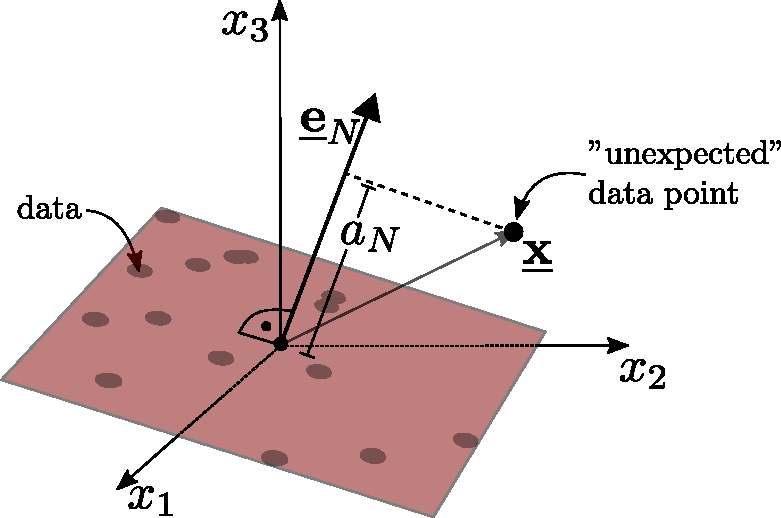
\includegraphics[width=6cm]{section1_fig6} 
\end{center}
%\pause
\begin{itemize}
        \itl outliers / data with novel features can be identified by projecting to last PCs
        \itl $y = \vec{e}_N^T \vec{x} =: a_N$ after learning $\leadsto$ projection onto smallest PC
        \itl large output for unexpected data $\rightarrow$ Novelty Filter
\end{itemize}

\paragraph{Novelty Filter: On-line Learning}
	\[ \begin{array}{ll}
	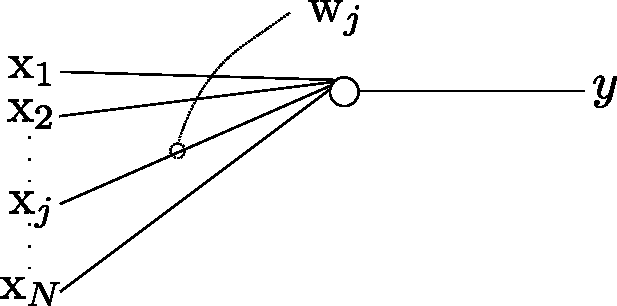
\includegraphics[width=5cm]{section2_fig5}
	& y = \vec{w}^T \vec{x}
	\end{array} \]
\textbf{Anti-Hebbian rule:} \\
\begin{equation}
				\Delta \mathrm{w}_j = \overbrace{-}^{\substack{	\text{''Anti''-} \\ \text{Hebbian} }} \varepsilon y^{(\alpha)} \mathrm{x}_j^{(\alpha)}
\end{equation}\\

Conjecture:\\ 
$\vec{w}$ converges to the direction of smallest eigenvector.\\
Proof:\\
Learning rule:
		\begin{equation}
		\Delta \mathrm{w}_j = - \varepsilon y^{(\alpha)} \mathrm{x}_j^{(\alpha)}
		\end{equation}
		Assume small learning steps $\rightarrow$ average over all patterns 
		\begin{equation}
			\Delta \mathrm{w}_j = - \frac{\varepsilon}{p} \sum_{\alpha = 1}^{p} y^{(\alpha)} \mathrm{x}_j^{(\alpha)} = - \frac{\varepsilon}{p} \sum_{\alpha = 1}^{p} \mathrm{x}_j^{(\alpha)} \sum_{k=1}^{N} \mathrm{x}_k^{(\alpha)} \mathrm{w}_k = - \varepsilon \sum_{k=1}^{N} C_{jk} \mathrm{w}_k 
		\end{equation}
		\begin{equation}
			\Delta \vec{w} = - \varepsilon \vec{C} \vec{w}
		\end{equation}

\begin{figure}[h]
\centering
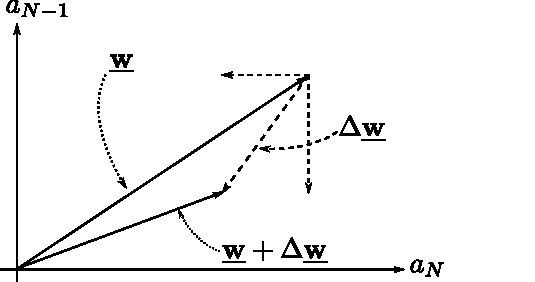
\includegraphics[width=7.5cm]{section2_fig6_a.pdf}
\end{figure}
Transformation into eigenbasis of covariance matrix:
\begin{align*}
			& \vec{w} = a_1 \vec{e}_1 + a_2 \vec{e}_2 + \dots + a_N \vec{e}_N\\
			& \Delta a_j = - \varepsilon \lambda_j a_j
s\end{align*}

\begin{itemize}
			\itl for $\lambda_j > 0: a_j \rightarrow 0$, constraints required
			\itl for $\lambda_j = 0: a_j$ remains unchanged
			\itl weights converge to the eigenvector with the smallest eigenvalue
\end{itemize}
\paragraph{Novelty Filter and linear regression}
\begin{center}
		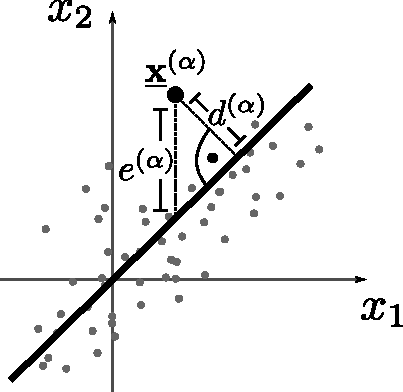
\includegraphics[width=3.6cm]{section2_fig6_b} \\
\end{center}
Ordinary least squares:\\
\begin{equation*}
		\frac{1}{p} \sum_{\alpha = 1}^{p} \left( e^{(\alpha)} \right)^2 \overset{!}{=} \text{min.}
\end{equation*}
\begin{itemize}
			\itl correct if data points are noisy along $x_2$-component only
			\itl wrong if data points are also noisy along $x_1$-component
\end{itemize}
total least squares:\\
\begin{equation*}
				\frac{1}{p} \sum_{\alpha =1}^{p} \left( d^{(\alpha)} \right)^2 \overset{!}{=} \text{min.}
\end{equation*}
tacit assumption: same variance noise \\
	centered data $\rightarrow \vec{w}^T\vec{x} = 0$ 

Cost function:
\begin{equation*}
		\mathbb{E}(\vec{w}) = \frac{1}{p} \sum_{\alpha =1}^{p} \left( d^{(\alpha)} \right)^2 \stackrel{!}{=} \min_{\vec{w}} \quad \text{s.t.} \abs{\vec{w}} = 1
\end{equation*}
\begin{equation*}
			\vec{w}^T \vec{C} \vec{w} \overset{!}{=} \min_{\vec{w}} \quad \text{s.t.} \abs{\vec{w}} = 1
\end{equation*}
\underline{solution}:\\
		$\vec{w}$ is the normalized eigenvector to the smallest eigenvalue of the covariance matrix.

\paragraph{Novelty Filter with normalization}
\begin{equation*}
		\Delta \vec{w} = - \varepsilon  \frac{y^{(\alpha)} \left\{ \vec{x}^{(\alpha)} - y^{(\alpha)} \vec{w} \right\}}{\abs{\vec{w} - \varepsilon y^{(\alpha)} \left\{ \vec{x}^{(\alpha)} - y^{(\alpha)} \vec{w} \right\}}}
\end{equation*}
Anti-Hebbian version of Oja's rule:\\
\begin{equation*}
			\Delta \mathrm{w}_j = - \varepsilon y^{(\alpha)} \Bigl\{ \overbrace{\mathrm{x}_j^{(\alpha)}}^{\substack{\text{Anti-Hebbian} \\ \text{learning}}} \underbrace{ - y^{(\alpha)} \mathrm{w}_j \Bigr\} + \varepsilon \Bigl\{ 1- \overbrace{\sum_{k=1}^{N} \mathrm{w}_k^2}^{=\abs{\vec{w}}^2} \Bigr\} \mathrm{w}_j}_{\text{normalization}}
\end{equation*}
\begin{itemize}
		\itl $\vec{w}$ converges to $\pm \vec{e}_N$
\end{itemize}

\paragraph{Feedforward network as a Novelty Filter}\mbox{}\\
Extension of the learning rule to N neurons:\\
\begin{equation*}
				\begin{aligned}
					\Delta \mathrm{w}_{ij} = 
					& - \varepsilon y_i^{(\alpha)} \Bigl\{ \mathrm{x}_j^{(\alpha)} - \overbrace{\sum_{k=1}^{i} \mathrm{w}_{kj} y_k^{(\alpha)}}^{-\sum_{k=1}^{i-1} \mathrm{w}_{kj} y_k^{(\alpha)} \text{is added}} \Bigr\} \\
					& + \varepsilon \Bigl\{ 1- \sum_{k=1}^{N} \mathrm{w}_{ik}^2 \Bigr\} \mathrm{w}_{ij}
				\end{aligned}
\end{equation*}
\begin{center}
\centering
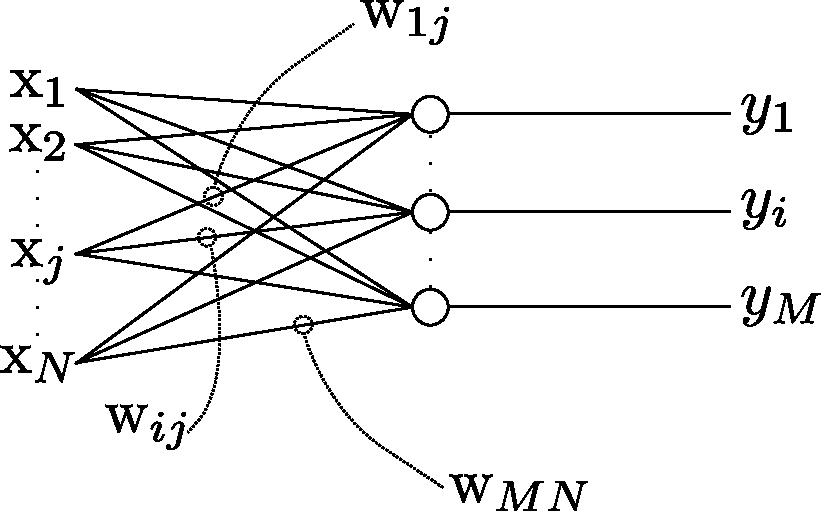
\includegraphics[width=0.5\textwidth]{section2_fig5_b}
\end{center}
\begin{tabular}{cll}
		$\leadsto$ result: & $\vec{w}_1 \rightarrow \vec{e}_N$ & (PC with smallest eigenvalue) \\ 
		& $\vec{w}_2 \rightarrow \vec{e}_{N-1}$ & $\vdots$ \\ 
		& $\vdots$ & $\vdots$ \\ 
		& $\vec{w}_M \rightarrow \vec{e}_{N-M+1}$ & (PC with largest eigenvalue, if $N=M$) \\ 
	\end{tabular}\\
	\vspace{0.3cm}
	Sequential calculation of eigenvectors (cf. Sanger's rule).

\paragraph{Recurrent network as a Novelty Filter}\mbox{}\\

\begin{figure}
\centering
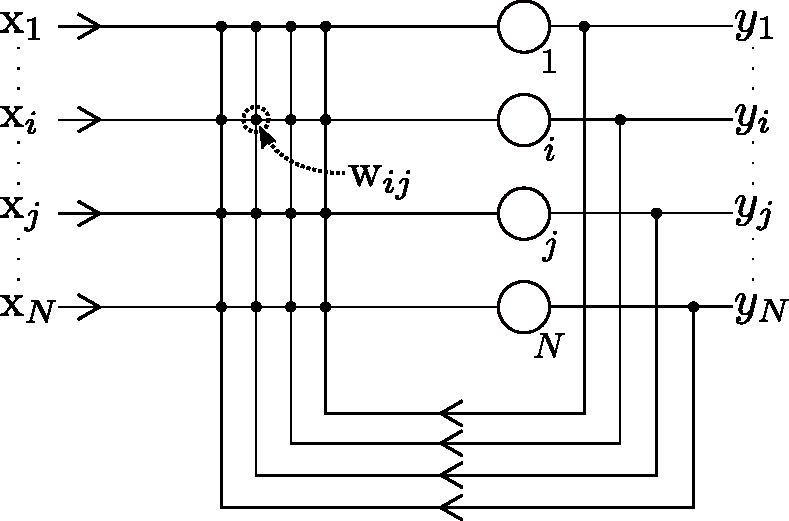
\includegraphics[width=5cm]{section2_fig25}
\end{figure}


\begin{tabular}{l}
				$y_i^{(\alpha)}(t+1) = \sum_{j=1}^{N} \mathrm{w}_{ij} y_j^{(\alpha)}(t) + \mathrm{x}_i^{(\alpha)}$ 	\\
				\raisebox{-0.2cm}{$\vec{y}^{(\alpha)}(t+1) = \vec{W} \vec{y}^{(\alpha)}(t) + \vec{x}^{(\alpha)}$}
\end{tabular}

Stationary state:\\
\begin{eqnarray*}
			&& \tilde{\vec{y}}^{(\alpha)}(t+1) = \tilde{\vec{y}}^{(\alpha)}(t) =: \tilde{\vec{y}}^{(\alpha)} \\
			&& \tilde{\vec{y}}^{(\alpha)} = \left( \vec{I} - \vec{W} \right)^{-1} \vec{x}^{(\alpha)}	
		\end{eqnarray*}
Convergence is guaranteed, if weight matrix is symmetric.\\
Learning rule:\\
\begin{center}
		$\Delta \mathrm{w}_{ij} = - \varepsilon \tilde{y}_i \tilde{y}_j$
\end{center}

\begin{figure}[h]
\centering 
\begin{subfigure}[b]{0.48\textwidth}
\centering
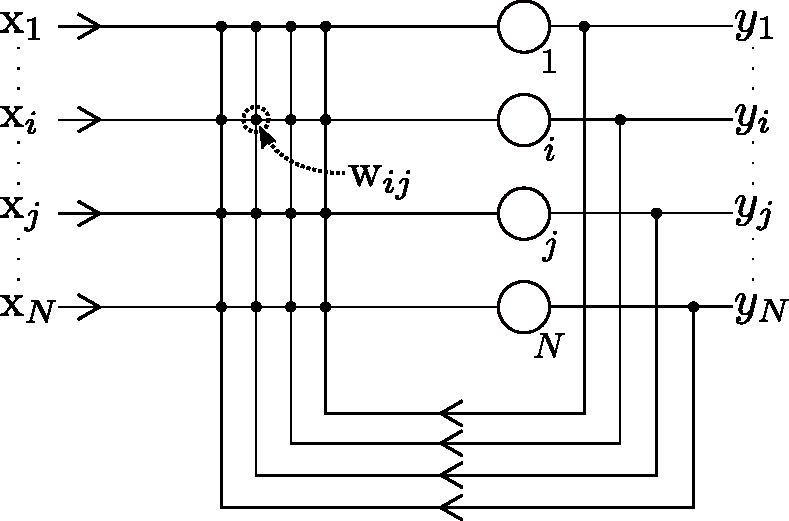
\includegraphics[width=5cm]{section2_fig25}
\\$\quad \tilde{\vec{y}}^{(\alpha)} = \left( \vec{I} - \vec{W} \right)^{-1} \vec{x}^{(\alpha)}$
\\$\quad \Delta \vec{w} = - \varepsilon \tilde{\vec{y}}^{(\alpha)} \left( \tilde{\vec{y}}^{(\alpha)} \right)^T$
\end{subfigure}
\begin{subfigure}[b]{0.48\textwidth}
\centering
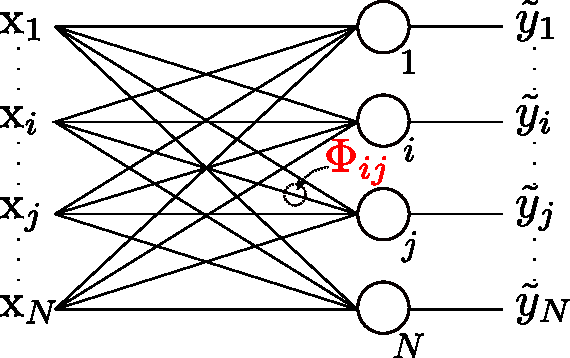
\includegraphics[width=5cm]{section2_fig26}
\\$\quad \tilde{\vec{y}}^{(\alpha)} = \vec{\Phi} \vec{x}^{(\alpha)}$
\\$\quad \Delta \vec{\Phi} = - \varepsilon \vec{\Phi}^2 \vec{x}^{(\alpha)} \left( \vec{x}^{(\alpha)} \right)^T \vec{\Phi}^2$
\end{subfigure}
\end{figure}

\paragraph{Recurrent network as a Novelty Filter - Algorithm}\mbox{}\\
\begin{algorithm}[H]
		\DontPrintSemicolon
		initialization of $\vec{\Phi}$ with identity matrix, $\vec{\Phi} = \vec{I}$\;
		\Repeat{convergence}{
			choose an observation  $\vec{x}^{(\alpha)}$\;
			change weight matrix according to:
			\vspace{-0.3cm}
			\begin{equation*}
			\Delta \vec{\Phi} = - \varepsilon \vec{\Phi}^2 \vec{x}^{(\alpha)} \left( \vec{x}^{(\alpha)} \right)^T \vec{\Phi}^2
			\end{equation*}    
			\vspace{-0.6cm}
		}
	\end{algorithm}

	\begin{itemize}
		\itl $\vec{\Phi}$ converges to a matrix, which projects onto the subspace orthogonal to the training data
	\end{itemize}

	\underline{example:}\\
	training data $\left\{ \vec{x}^{(1)}, \dots, \vec{x}^{(p)} \right\} \subseteq \operatorname{span}\left\{ \vec{e}_1, \dots, \vec{e}_{N-1} \right\} \qquad \vec{x}^{(\alpha)} \in \mathbb{R}^N$
	\vspace{-0.2cm}
	\begin{equation*}
		\vec{\Phi} \xrightarrow[t \to \infty]{} \vec{I} - \sum_{k=1}^{N-1} \vec{e}_k \vec{e}_k^T \leadsto \vec{\Phi} \vec{e}_j = \vec{e}_N \delta_{jN} \leadsto \vec{\Phi} \vec{x} = \underbrace{\left( \vec{e}_N^T \vec{x} \right)}_{=: a_N} \vec{e}_N
	\end{equation*}

\paragraph{Recurrent network as a Novelty Filter - Neural facial expressions}\mbox{}\\
\begin{figure}[h]
		\centering
			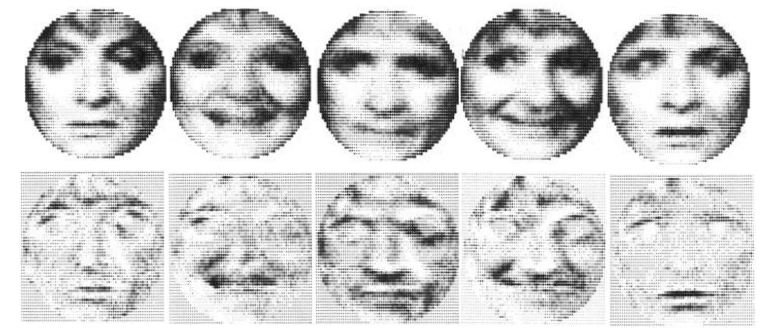
\includegraphics[width=0.8\textwidth]{novelty_faces_cropped.png}
		\caption*{\hspace{5cm} \textit{(taken from Kohonen 1989)}}
	\end{figure}

	\vspace{-0.5cm}
	\begin{itemize}
		\item training data: ''neutral'' facial expressions (not shown here)
		\begin{itemize}
			\itl $\vec{\Phi}$ projects into space orthogonal to this data
		\end{itemize}
		\item top row: faces $\vec{x}^{(\beta)}$ with different expressions
		\item bottom row: projection $\vec{\Phi} \vec{x}^{(\beta)}$
	\end{itemize}

\paragraph{Novelty Filter: Summary}\mbox{}\\
	\textbf{One neuron:}
	\[ \begin{array}{ll}
	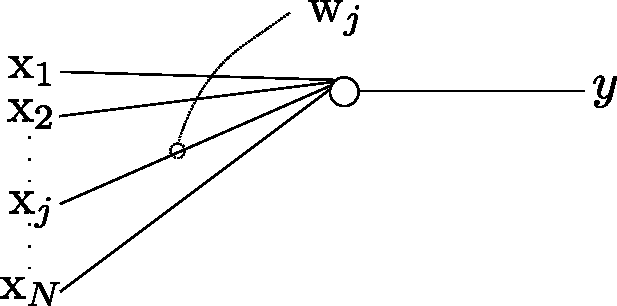
\includegraphics[width=5cm]{section2_fig5}
	& y = \vec{w}^T \vec{x}
	\end{array} \]
	\textbf{Anti-Hebbian learning rule}
		\begin{equation*}
			\Delta \mathrm{w}_j = - \varepsilon y^{(\alpha)} \Bigl\{ \overbrace{\mathrm{x}_j^{(\alpha)}}^{\substack{\text{Anti-Hebbian} \\ \text{learning}}} \underbrace{ - y^{(\alpha)} \mathrm{w}_j \Bigr\} + \varepsilon \Bigl\{ 1- \overbrace{\sum_{k=1}^{N} \mathrm{w}_k^2}^{=\abs{\vec{w}}^2} \Bigr\} \mathrm{w}_j}_{\text{normalization}}
		\end{equation*}
		
\textbf{$N$ neurons:}\\
	\begin{center}
	 \begin{tabular}{ll}
		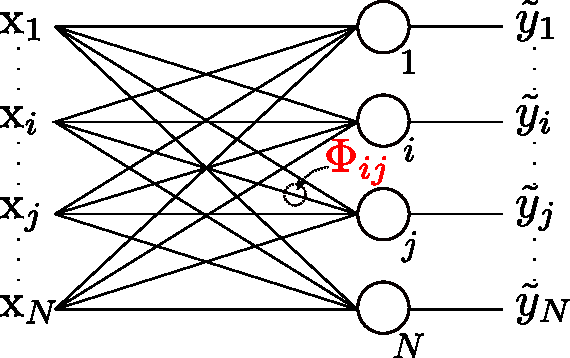
\includegraphics[width=5.5cm]{section2_fig26}
		& \raisebox{1cm}{$\tilde{\vec{y}}^{(\alpha)} = \vec{\Phi} \vec{x}^{(\alpha)}$}
	\end{tabular} 
	\end{center}
	\textbf{Learning rule:}
		\begin{equation*}
			\Delta \vec{\Phi} = - \varepsilon \vec{\Phi}^2 \vec{x}^{(\alpha)} \left( \vec{x}^{(\alpha)} \right)^T \vec{\Phi}^2
		\end{equation*}
		\vspace{-0.5cm}
		\begin{itemize}
			\itl $\vec{\Phi}$ converges to projection matrix onto subspace orthogonal to training data
		\end{itemize}
		
		
% -----------------------------------------------------------------------------

\newpage 						% for visual reasons
\section{Independent Component Analysis}
% -----------------------------------------------------------------------------
\subsection{Independent Component Analysis}
\label{sec:ICA}
The methods described in this section use a linear generative model to extend decorrelation methods like PCA to find statistically independent sources.\\\\
\textbf{The cocktail party problem:} linear superposition of sources

\begin{figure}[h]
  \centering
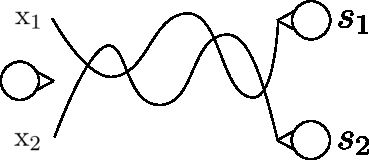
\includegraphics[width=5cm]{section2_fig10}  
\begin{equation}
	\underbrace{ \vec{x} }_{ \text{observations} } 
	= \underbrace{ \vec{A} }_{ \substack{ 	\text{mixing} \\
						\text{matrix}} }
	\underbrace{ \vec{s} }_{ \text{sources} }
\end{equation}

  \caption{The cocktail party problem}
  \label{fig:cocktailParty}
\end{figure}


\paragraph{Question:}
Can we recover the sources from the observations - with no prior knowledge about the mixing process (i.e. the matrix $\vec{A}$)?
\\\\
Yes - but we need to make assumptions about the statistical properties of the sources. 
\begin{itemize}
	\itl source separation methods differ in what prior knowledge they exploit
\end{itemize}

\begin{table}[h]
  \centering
\fbox{
  \begin{tabular}{>{$}c<{$}c c c >{$}c<{$}}
  Approach\; 1 \; \textrm{(direct)}
    && $\vec{x}^{(\alpha)}\; \overset{\mathrm{iid}}{\sim} P_{\vec{x}}(\vec{x})$  
    & &Approach\; 2 \; \textrm{(Infomax)} \\
  & & Data   & &\\ 
  & & $\Downarrow$ & &\\ 
% P_{\vec{s}}(\hat{\vec{s}}),\; \; 
\hat{\vec{s}}:=\vec{W}\, \vec{x}    & & 
  Models & &  \hat{u}_i := \hat f_i( \overbrace{e_i^T\vec{W}\, \vec{x}}^{=: \hat s_i})\\ 
   & & $\Downarrow$ && \\ 
D_\textrm{KL}(P_{\vec{s}}(\hat{\vec{s}}) \; || \; \prod_i P_{s_i}(\hat{s_i}) )   & & Performance measure && H(\hat{\vec{u}})\\ 
   & & $\Downarrow$ && \\ 
\displaystyle \min_{\vec{W}} D_\textrm{KL}   & & Optimization &&  \displaystyle \max_{\vec{W}} H(\hat{\vec{u}})\\ 
  \end{tabular}
}
  \caption{Overview of the 2 approaches: Note that the two approaches are equivalent if the 
  ``transition functions'' $\hat f_i$ match the marginal distribution functions of the 
  true independent sources i.e. $f_i = cdf(s_i)$.}
  \label{tab:approach}
\end{table}

\paragraph{Goal:} recovery of independent sources $\hat{S}$ from observations

\paragraph{Procedure:}
Given observations $\vec{x}$, find $\vec{W}$ with 
\begin{equation}
	\underbrace{ \widehat{\vec{s}} }_{ \substack{ 	\text{''estimated} \\
							\text{sources''}} }
	= \underbrace{ \vec{W} }_{ \substack{	\text{''unmixing} \\
						\text{matrix''}} }
	\underbrace{ \vec{x} }_{ \text{observations} }
\end{equation}
such that the joint distribution of sources factorizes:
\begin{equation}
	P_{\vec{s}} (\widehat{\vec{s}}) 
	= \prod_{i = 1}^N P_{\vec{s}}(\widehat{s_i})
\end{equation}
In the special case of a noise-free mixing process, this means:
\begin{equation}
	\vec{W} = \vec{A}^{-1}
\end{equation}


\paragraph{Why not PCA?} Decorrelation is not independence!

\begin{figure}[h]
  \centering
$P_{\vec{s}}(\vec{s})=P_{s_1}(s_1)\cdot P_{s_2}(s_2)$
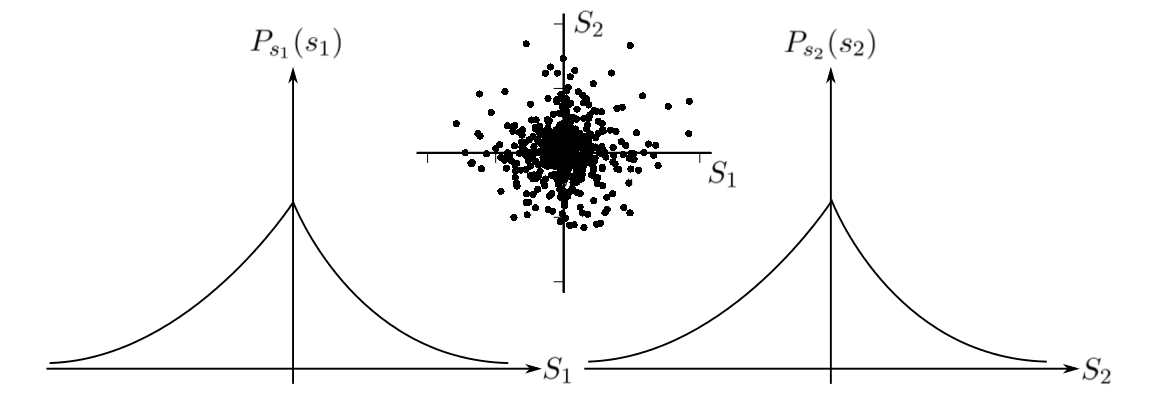
\includegraphics[width=14cm]{section2_fig11mod}  
  \caption{Marginal and joint distribution of independent variables}
  \label{fig:jointMarginal}
\end{figure}


\begin{equation}
	\vec{x} = \vec{A} \vec{s} = \left( \begin{array}{ll}
			a_{11} & a_{12} \\ a_{21} & a_{22}
		\end{array} \right) \cdot \left( \begin{array}{ll}
			s_1 \\ s_2
		\end{array} \right)
	= \left( \begin{array}{l}
		a_{11} s_1 + a_{12} s_2 \\ a_{21} s_1 + a_{22} s_2
	\end{array} \right)
\end{equation}
let $\vec{A} = \big( \vec{a}_1, \vec{a}_2 \big)$:
\begin{equation}
	\begin{array}{ll}
	\vec{s} = \left( \begin{array}{l} 1 \\ 0 \end{array} \right) 
		\leadsto \vec{x} = \left( \begin{array}{l} 
		a_{11} \\ a_{21} \end{array} \right) = \vec{a}_1
		& \text{1st source} 
		\\\\
	\vec{s} = \left( \begin{array}{l} 0 \\ 1 \end{array} \right) 
		\leadsto \vec{x} = \left( \begin{array}{l} 
		a_{12} \\ a_{22} \end{array} \right) = \vec{a}_2
		& \text{2nd source}
	\end{array}
\end{equation}
\begin{figure}[h]
  \centering
  \begin{tabular}{c c}
  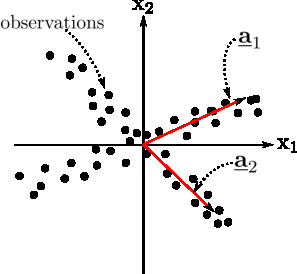
\includegraphics[height=4.85cm]{section2_fig12}  &     
  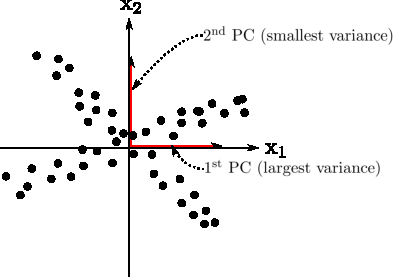
\includegraphics[height=4.8cm]{section2_fig13}
  \end{tabular}
  \caption{Motivation for ICA: In a set of observations, sources are ''interesting'' directions in feature space
    (left). Decorrelation (e.g. through PCA, right), might not find the relevant directions $\Rightarrow$ new  methods needed!}

  \label{fig:icaExample1}
\end{figure}



\paragraph{Limits to recovery}
\begin{enumerate}[(1)]
\item permutations of sources
\begin{equation*}
	\begin{array}{ccc}
	\left( \begin{array}{ll}
		\widehat{s}_1 \\ \widehat{s}_2
	\end{array} \right)
	=
	\left( \begin{array}{ll}
		\mathrm{w}_{11} & \mathrm{w}_{12} \\
		\mathrm{w}_{21} & \mathrm{w}_{22} 
	\end{array} \right)
	\left( \begin{array}{ll}
		\mathrm{x}_1 \\ \mathrm{x}_2
	\end{array} \right)
	& \corresponds &
	\left( \begin{array}{ll}
		\widehat{s}_2 \\ \widehat{s}_1
	\end{array} \right)
	=
	\left( \begin{array}{ll}
		\mathrm{w}_{21} & \mathrm{w}_{22} \\
		\mathrm{w}_{11} & \mathrm{w}_{12} 
	\end{array} \right)
	\left( \begin{array}{ll}
		\mathrm{x}_1 \\ \mathrm{x}_2
	\end{array} \right)
	\\\\
	P_{s_1} (\widehat{s}_1) \cdot P_{s_2} (\widehat{s}_2)
	&& 
	P_{s_2} (\widehat{s}_2) \cdot P_{s_1} (\widehat{s}_1)
	\end{array}
\end{equation*}
\indent both alternatives are solutions to the unmixing problem
\item amplitude of the sources
\begin{equation*}
	\begin{array}{ccc}
	\left( \begin{array}{ll}
		\widehat{s}_1 \\ \widehat{s}_2
	\end{array} \right)
	=
	\left( \begin{array}{ll}
		\mathrm{w}_{11} & \mathrm{w}_{12} \\
		\mathrm{w}_{21} & \mathrm{w}_{22} 
	\end{array} \right)
	\left( \begin{array}{ll}
		\mathrm{x}_1 \\ \mathrm{x}_2
	\end{array} \right)
	& \corresponds &
	\left( \begin{array}{ll}
		a\widehat{s}_1 \\ b\widehat{s}_2
	\end{array} \right)
	=
	\left( \begin{array}{ll}
		a\mathrm{w}_{11} & a\mathrm{w}_{12} \\
		b\mathrm{w}_{21} & b\mathrm{w}_{22} 
	\end{array} \right)
	\left( \begin{array}{ll}
		\mathrm{x}_1 \\ \mathrm{x}_2
	\end{array} \right)
	\\\\
	P_{s_1} (\widehat{s}_1) \cdot P_{s_2} (\widehat{s}_2)
	&& 
	P_{s_1} (a\widehat{s}_1) \cdot P_{s_2} (b\widehat{s}_2)
	\end{array}
\end{equation*}
\indent both alternatives are solutions to the unmixing problem
\\\\
\item Gaussian distributions for sources and observations
\begin{equation*}
	\widehat{\vec{s}} = \vec{W} \vec{x} 
\end{equation*}
Assuming whitened variables, the probability depends only on the length of the vector, i.e.\ distance of the point from the origin. 
\begin{equation}
	\begin{array}{ll}
	P_{\vec{s}}(\widehat{\vec{s}}) 
	& = \frac{1}{2\pi} \exp \bigg\{ -\frac{\widehat{\vec{s}}^2}{2} \bigg\}
	\\\\
	& = \underbrace{ \Bigg[ \frac{1}{\sqrt{2\pi}} \exp \bigg\{ -
		\frac{\widehat{s_1}^2}{2} \bigg\} \Bigg] \Bigg[
			\frac{1}{\sqrt{2\pi}} \exp \bigg\{ -
			\frac{\widehat{s_2}^2}{2} \bigg\}
		\Bigg] }_{\text{solution to the unmixing problem} }
	\end{array}
\end{equation}
\indent let $\vec{B}$ be an orthogonal matrix: $\vec{B}^T \vec{B} = \vec{1}$
\begin{equation}
	\begin{array}{ll}
		\widetilde{\vec{s}} 
		& = \vec{B} \widehat{\vec{s}} \\\\
		& = \vec{B} \vec{W} \vec{x} \\\\
		& = \vec{W'} \vec{x}
	\end{array}
\end{equation}
\begin{equation}
	\begin{array}{ll}
		\widetilde{\vec{s}}^2:=\|\widetilde{\vec{s}}\|_2^2 
		& = \sum\limits_{i = 1}^2 \widetilde{s}_i^2 \\\\
		& = \sum\limits_{i,k,l = 1}^2 B_{ik} \widehat{s}_k B_{il} \widehat{s}_l
			\\\\
		& = \sum\limits_{k,l = 1}^2 \widehat{s}_k
			\bigg( \sum\limits_{i = 1}^2 B_{ki}^T B_{il} \bigg)
			\widehat{s}_l \\\\
		& = \widehat{\vec{s}}^T 
			\underbrace{ \big( \vec{B}^T \vec{B} \big) }_{
				\eqexcl \vec{1} } \widehat{\vec{s}} \\\\
		& = \widehat{\vec{s}}^2
	\end{array}
\end{equation}
\begin{equation}
	\widetilde{\vec{s}} = \vec{W}' \vec{x}
\end{equation}
\begin{equation}
	\begin{array}{ll}
	P_{\vec{s}}(\widetilde{\vec{s}}) 
	& = \frac{1}{2\pi} \exp \bigg\{ -\frac{\widetilde{\vec{s}}^2}{2} \bigg\}
	\\\\
	& = \underbrace{ \Bigg[ \frac{1}{\sqrt{2\pi}} \exp \bigg\{ -
		\frac{\widetilde{s_1}^2}{2} \bigg\} \Bigg] \Bigg[
			\frac{1}{\sqrt{2\pi}} \exp \bigg\{ -
			\frac{\widetilde{s_2}^2}{2} \bigg\}
		\Bigg] }_{\text{also solution to the unmixing problem} }
	\end{array}
\end{equation}
\end{enumerate}
% -----------------------------------------------------------------------------

\subsection[Model-based Source Separation]{Model-based Source Separation Techniques}
\subsubsection{The Infomax Principle}
observations: $\vec{x} \in \mathbb{R}^N, P_{\vec{x}}(\vec{x}) \leftarrow$ true (unknown) density 
\\\\
estimated sources: $\widehat{\vec{s}} = \vec{W} \vec{x}, \widehat{\vec{s}} \in \mathbb{R}^N, \vec{W}$ regular $N \times N$ matrix
\begin{itemize}
	\itl $P_{\vec{s}}(\widehat{\vec{s}})$: family of true (unknown) 
		densities, parametrized by $\vec{W}$
\end{itemize}
\paragraph{Approach 1: direct model selection} (cf. section \ref{sec:ParametricDensityEstimation})
\begin{itemize}
\item[\emph{Idea:}]select the model, which yields a distribution most similar to a factorizing density
\end{itemize}
\begin{equation}
	\widehat{P}_{\vec{s}}(\widehat{\vec{s}}) 
	= \prod_{i = 1}^N \widehat{P}_{s_i}(\widehat{s}_i)
	\leftarrow \text{ ICA assumption}
\end{equation}
This naturally leads to formulation of the following cost function
\begin{equation}
	\dkl = \int d \widehat{\vec{s}} P_{\vec{s}}(\widehat{\vec{s}})
		\ln \frac{P_{\vec{s}}(\widehat{\vec{s}})}{
			\prod_{i = 1}^N \widehat{P}_{s_i}(\widehat{s}_i) }
		\eqexcl \min
\end{equation}
which could be directly optimized. 
But: estimation of $\vec{W} \; \corresponds$ estimation of the probability density $P_{\vec{s}}(\widehat{\vec{s}})$
\begin{itemize}
	\itl parametrized density estimate required (which can be expensive)
\end{itemize}



\paragraph{Approach 2: Information Maximization (Bell \& Sejnowski, 1995)}
\label{sec:ICA-BellSejnowski}
\begin{itemize}
\item[\emph{Idea:}] Under certain conditions, maximizing the
  \emph{mutual information} between inputs (mixed signals) and outputs
  (recovered sources) of a system yields \emph{independent} outputs.\footnote{For a more detailed description of this argument, see \textcite{BellSejnowski1995}.} Note that if sources are independent, then
  transformations of these sources are independent, too.
\item[$\leadsto$] Choosing the transformation in a clever way (such
  that their marginal distributions become uniform, see below)
  simplifies the computations to find independent sources.
\end{itemize}
\emph{Excursion on Density Transformations:} We will see that
computations simplify if we choose a transformation $\widehat{f}_i$
leading to uniformly distributed sources, i.e. $\widehat{u}_i =
\widehat{f}_i(\widehat{s}_i)$, such that
$\widehat{P}_{u_i}(\widehat{u}_i) = \mathrm{const.}$
\\\\
The transformation can be found using \emph{conservation of probability}
\begin{equation}
	\widehat{P}_{u_i}(\widehat{u}_i) d \widehat{u}_i 
	\; =  \; \widehat{P}_{s_i} (\widehat{s}_i) d \widehat{s}_i.
\end{equation}
Using the general rule for density transformations and applying it here yields
\begin{equation}
	\widehat{P}_{u_i}(\widehat{u}_i) \quad
	 =  \quad \bigg| 
		\frac{d \widehat{s}_i}{d \widehat{u}_i} \bigg| 
			 \widehat{P}_{s_i}(\widehat{s}_i) \quad
	 =  \quad \frac{1}{\big| \widehat{f}_i^{'} (\widehat{s}_i) \big|} 
		\widehat{P}_{s_i}(\widehat{s}_i)
\end{equation}
where $\left|\frac{d \widehat{s}_i}{d \widehat{u}_i} \right|$ is
called \emph{functional determinant} of the transformation
$\widehat{f}_i$. For a general transformation, this is illustrated in
figure \ref{fig:densityTransformation}.
\begin{figure}[h]
  \centering
  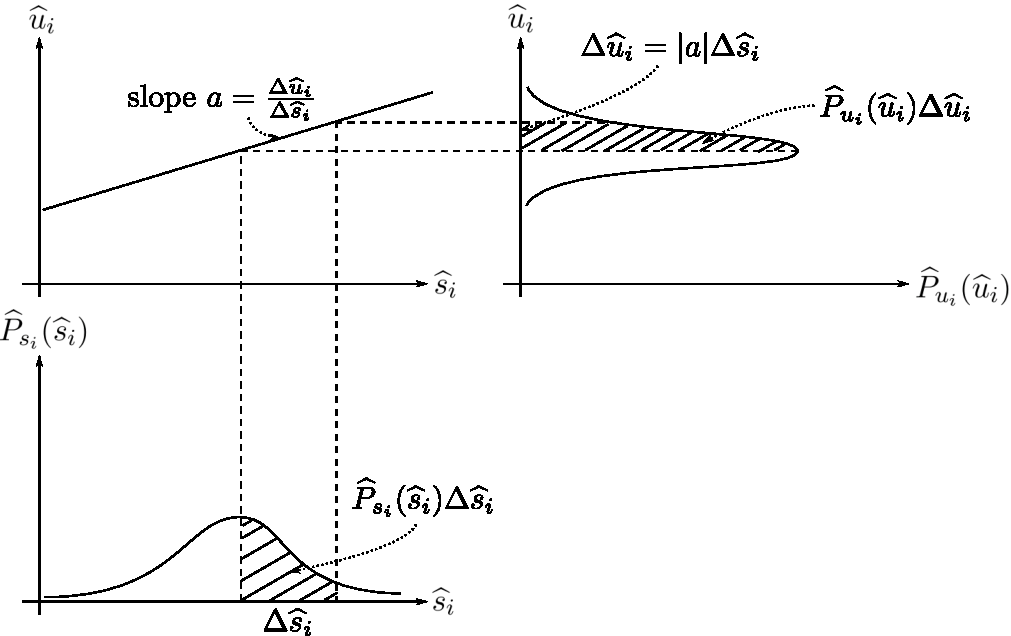
\includegraphics[width=\linewidth]{section2_fig14}  
  \caption{Illustration of a density transformation}
  \label{fig:densityTransformation}
\end{figure}
Applying the principle of conservation of probability (equal size
areas) to find a transformation resulting in a uniformly distributed
variable with a constant density yields: 
\begin{equation}
  \label{eq:1}
		\widehat{P}_{u_i} (\widehat{u}_i) \; = \;   
		 \frac{1}{\big| \widehat{f}_i^{'} (\widehat{s}_i) \big|} 
		\widehat{P}_{s_i}(\widehat{s}_i) \; \stackrel{!}{=} \; const \qquad \Rightarrow \qquad 
		 \big| \widehat{f}_i^{'} (\widehat{s}_i) \big| =  a \widehat{P}_{s_i}(\widehat{s}_i) 
\end{equation}
and therefore
\begin{equation}
\Rightarrow \widehat{f}_i (\widehat{s}_i)
 = \int\limits_{-\infty}^{\widehat{s}_i} dy\; a 
			\widehat{P}_{s_i}(y)
\end{equation}

\begin{figure}[h]
  \centering
  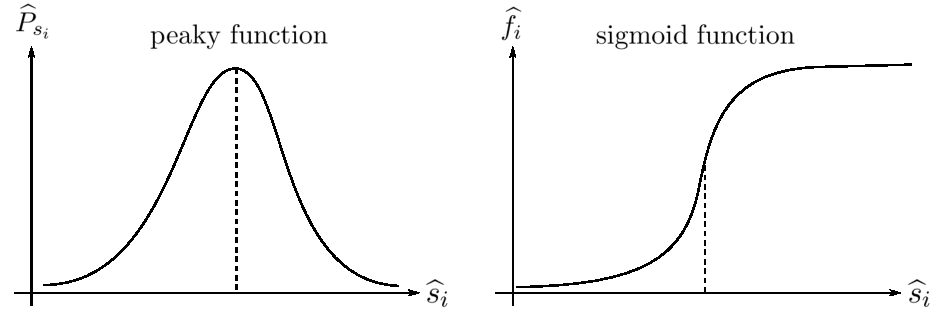
\includegraphics[width=12cm]{section2_fig15}  
  \caption{density (pdf) and corresponding distribution function (cdf)}
  \label{fig:cdf}
\end{figure}

\paragraph{Application of density transformations to solve the ICA problem:}
\label{sec:appl-dens-transf}
KL-divergence for the transformed densities:
\begin{eqnarray}
  \dkl & = & \int d \vec{s} P_{\widehat{\vec{s}}} \ln \frac{P_{\widehat{\vec{s}}}}{\prod_i P_{\widehat{s_i}}}\\
  & = &  \int d \vec{s} P_{\widehat{\vec{s}}} \ln \frac{P_{\widehat{\vec{s}}} \quad \prod_i \frac{1}{f_i'}}{\prod_i  P_{\widehat{s_i}} \quad \frac{1}{f_i'}}
  \quad = \int d \vec{u} P_{\widehat{\vec{u}}} \ln \frac{P_{\widehat{\vec{u}}}}{\prod_i  P_{\widehat{u_i}}} \\
  & = &  \underbrace{ \int d \widehat{\vec{u}} P_{\vec{u}}
    (\widehat{\vec{u}}) \ln P_{\vec{u}}(\widehat{\vec{u}}) }_{
    \substack{ = -H(u) \\ \text{negative entropy} \\
      \text{of the transformed} \\
      \text{(true) density}} }
  -\int d \widehat{\vec{u}} P_{\vec{u}}
  (\widehat{\vec{u}}) \Bigg(\underbrace{ \ln \prod\limits_{i = 1}^N
    \widehat{P}_{u_i} (\widehat{u}_i)}_{
    \text{const. for 'flat' $u_i$} }\Bigg) 
\end{eqnarray}
This motivates the socalled \emph{Infomax principle} \parencite{BellSejnowski1995}
\begin{equation}\label{eq:infomax}
  H = -\int d \widehat{\vec{u}} P_{\vec{u}} (\widehat{\vec{u}})
  \ln P_{\vec{u}} (\widehat{\vec{u}}) \eqexcl \max 
\end{equation}
using the transformed estimated sources
\begin{equation}
\widehat{u}_i = \widehat{f}_i \big( \underbrace{ \vec{e}_i^T
		\vec{W} \, \vec{x}  }_{= \widehat{s_i} } \big) 
\end{equation}

% -----------------------------------------------------------------------------

\subsubsection{ICA via Neural Networks and Empirical Risk Minimization}
\[ \begin{array}{ll}
	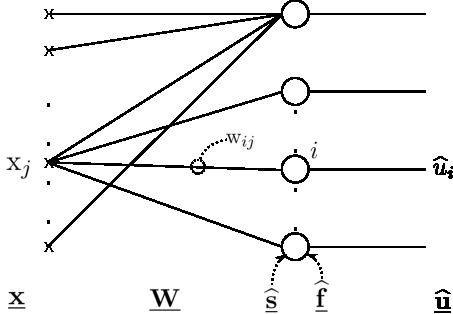
\includegraphics[width=7cm]{section2_fig16}
	& \begin{array}{l}
		\text{perceptron network} \\\\
		u_i = \underbrace{ \widehat{f}_i 
				\Big( \sum\limits_j \mathrm{w}_{ij} 
					\mathrm{x}_j \Big) }_{
					\substack{ \text{often a} \\
						   \text{sigmoid function}} }
				\\\\
		\text{observations: } \vec{x}^{(\alpha)} \in \mathbb{R}^N, 
			\alpha = 1, \ldots, p \\\\
		\rightarrow \substack{	\text{determine the weights} \\
					\text{through inductive learning}}
	\end{array}
\end{array} \]
derivation of the cost function
\begin{equation}
	P_{\vec{u}} (\widehat{\vec{u}}) d \widehat{\vec{u}}
		= P_{\vec{x}}(\vec{x}) d \vec{x}
\end{equation}
\begin{equation}
	\begin{array}{ll}
	P_{\vec{u}} (\widehat{\vec{u}}) 
	& = \left| \frac{d \vec{x}}{d \widehat{\vec{u}}} \right|
		P_{\vec{x}}(\vec{x}) \\\\
	& = \frac{P_{\vec{x}}(\vec{x})}{ \left| 
		\frac{d \widehat{\vec{u}}}{d \vec{x}} \right|}
       = \frac{P_{\vec{x}}(\vec{x})}{|\mathbf{M}|}
	\end{array}
\end{equation}
with elements of the functional determinant $\mathbf{M}$ being given as
\begin{equation}
	\begin{array}{ll}
 \mathbf{M}_{ij}=	\frac{\partial \widehat{u}_i}{\partial \mathrm{x}_j}
	& = \frac{\partial}{\partial \mathrm{x}_j} 
		\widehat{f}_i \bigg( \sum\limits_{k = 1}^N \mathrm{w}_{ik} 
		\mathrm{x}_k \bigg) \\\\
	& = \mathrm{w}_{ij} \widehat{f}_i^{'} \bigg( \sum\limits_{k = 1}^N 
		\mathrm{w}_{ik} \mathrm{x}_k \bigg).
	\end{array}
\end{equation}
We therefore obtain for the value of the functional determinant
\begin{equation} \label{eq:functionalDeterminant}
|\mathbf{M}| = 
	\Big| \frac{\partial \widehat{\vec{u}}}{\partial \vec{x}} \Big|
	= |\vec{w}| \prod\limits_{l = 1}^N  \widehat{f}_l^{'} \Bigg( 
		\sum\limits_{k = 1}^N \mathrm{w}_{lk} \mathrm{x}_k \Bigg).
\end{equation}
Inserting this into the Infomax cost function (\ref{eq:infomax}) gives 
\begin{eqnarray}
H & = & -\int d \widehat{\vec{u}} P_{\vec{u}} (\widehat{\vec{u}})
  \ln P_{\vec{u}} (\widehat{\vec{u}}) \\
& = &  
-\int d \vec{x} P_{\vec{x}} (\vec{x}) \ln \frac{P_{\vec{x}}(\vec{x})}{|\mathbf{M}|} \\
& = & 
\underbrace{-\int d \vec{x} P_{\vec{x}} (\vec{x}) \ln P_{\vec{x}}(\vec{x})}_{ \text{constant w.r.t. } \vec{w} } +
\int d \vec{x} P_{\vec{x}} (\vec{x}) \ln |\mathbf{M}|
\end{eqnarray}
and with~(\ref{eq:functionalDeterminant}) can be written in terms explicitly depending on w:
\begin{equation}
	H = const + \int d \vec{x} P_{\vec{x}} (\vec{x}) \ln |\vec{w}|
		+ \int d \vec{x} P_{\vec{x}} (\vec{x}) \sum\limits_{l = 1}^N
			\ln \widehat{f}_l^{'} \Bigg( \sum\limits_{k = 1}^N 
			\mathrm{w}_{lk} \mathrm{x}_k \Bigg).
\end{equation}
As mentioned above, the entropy can then be used for model selection:
\begin{equation} \tag{generalization cost}
	E^G = \ln |\vec{w}| + \int d \vec{x} P_{\vec{x}} (\vec{x})
		\Bigg\{ \sum\limits_{l = 1}^N \ln
			\widehat{f}_l^{'} \Bigg( \sum\limits_{k = 1}^N 
			\mathrm{w}_{lk} \mathrm{x}_k \Bigg)
		\Bigg\}
\end{equation}
Via the \emph{principle of empirical risk minimization}
\begin{center}
mathematical expectation $E^G \longrightarrow$ empirical average $E^T$
\end{center}
the \emph{training cost}
\begin{equation} \label{eq:trainingCost}
	E^T = \ln |\vec{w}| + \frac{1}{p} \sum\limits_{\alpha = 1}^p
		\sum\limits_{l = 1}^N \ln \widehat{f}_l^{'} \Bigg( 
		\sum\limits_{k = 1}^N \mathrm{w}_{lk} 
		\mathrm{x}_k^{(\alpha)} \Bigg)
\end{equation}
can be used for model selection using empirical data 
\begin{equation}
	\fbox{$ E^T \eqexcl \max $}
\end{equation}

% -----------------------------------------------------------------------------

\subsubsection{Learning by Gradient Ascent}
Model parameters can be optimized by stepwise adustment along the direction of the gradient of the cost function. 

\begin{figure}[h]
  \centering
  \begin{tabular}[c c]{c c}
   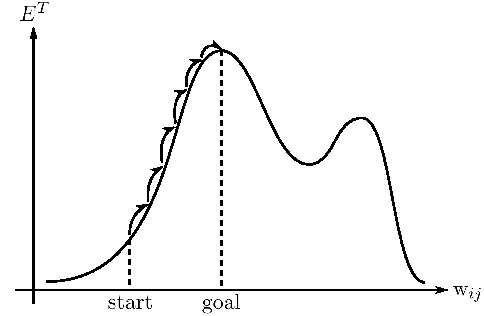
\includegraphics[width=7cm]{section2_fig17}
  &\raisebox{2cm}{$\Delta \mathrm{w}_{ij} = \underbrace{ \eta }_{
    \substack{ \text{learning} \\ \text{step}} }
  \frac{\partial E^T}{\partial \mathrm{w}_{ij}}$}
  \end{tabular}  
  \caption{Gradient descent using the training cost}
  \label{fig:gradientDescent}
\end{figure}
\noindent Taking partial derivatives of the training cost (\ref{eq:trainingCost}) wrt. the model parameters $w_{ij}$ yields
\begin{equation}
	\frac{\partial E^T}{\partial \mathrm{w}_{ij}}
	= \underbrace{ \frac{1}{p} \sum\limits_{\alpha = 1}^p 
		\sum\limits_{l = 1}^N \frac{\partial}{\partial \mathrm{w}_{ij}}
		\Bigg\{ \ln \widehat{f}_l^{'} \Bigg( \sum\limits_{k = 1}^N 
		\mathrm{w}_{lk} \mathrm{x}_k^{(\alpha)} \Bigg) \Bigg\} }_{
			\frac{1}{p} \sum\limits_{\alpha = 1}^p 
			\frac{ \widehat{f}_i^{''} \Big( \sum\limits_{k = 1}^N 
				\mathrm{w}_{ik} \mathrm{x}_k^{(\alpha)} \Big)
			}{\widehat{f}_i^{'} \Big( \sum\limits_{k = 1}^N 
			\mathrm{w}_{ik} \mathrm{x}_k^{(\alpha)} \Big)}
			\cdot \mathrm{x}_j^{(\alpha)} }
		+ \underbrace{ \frac{\partial}{\partial \mathrm{w}_{ij}}
			\big( \ln |\vec{w}| \big) }_{
				\big( \vec{w}^{-1} \big)_{ji} }
\end{equation}
with individual costs:
\begin{equation}
	e^{(\alpha)} = \ln |\vec{w}| + \sum\limits_{l = 1}^N \ln
		\widehat{f}_l^{'} \Bigg( \sum\limits_{k = 1}^N 
		\mathrm{w}_{lk} \mathrm{x}_k^{(\alpha)} \Bigg)
\end{equation}
\begin{equation}
	\frac{\partial e^{(\alpha)}}{\partial \mathrm{w}_{ij}}
	= \underbrace{ \big( \vec{w}^{-1} \big)_{ji} }_{
		\substack{ \text{costly} \\ \text{computation}} }
		+ \underbrace{  
			\frac{ \widehat{f}_i^{''} \bigg( \sum\limits_{k = 1}^N 
				\mathrm{w}_{ik} \mathrm{x}_k^{(\alpha)} \bigg)
			}{\widehat{f}_i^{'} \bigg( \sum\limits_{k = 1}^N 
			\mathrm{w}_{ik} \mathrm{x}_k^{(\alpha)} \bigg)}
			 }_{ \coloneqq \varphi_i^{(\alpha)} }
		\cdot \mathrm{x}_j^{(\alpha)}
\end{equation}
this can be used for \emph{batch-learning}:
\begin{equation}
	\Delta \mathrm{w}_{ij}
	= \frac{\eta}{p} \sum\limits_{\alpha = 1}^p 
	\frac{\partial e^{(\alpha)}}{\partial \mathrm{w}_{ij}}
\end{equation}
or using \emph{on-line-learning} (see algorithm~\ref{alg:onlineGD}).\footnote{see also MI I, chapters 1.3.4 and 1.4.1-1.4.3}
\begin{algorithm}
  \DontPrintSemicolon
  $t \leftarrow 1$\;
  random initialization of weights $w_{ij}$\;
  \Begin{
    $\eta_t = \frac{\eta_0}{t}$\;
    select next data point $\vec{x}^{(\alpha)}$\;
    change all  $\mathrm{w}_{ij}$ according to:
    $\Delta \mathrm{w}_{ij}^{(t)} = \eta_t \frac{\partial e_t^{(\alpha)}}{\partial
	\mathrm{w}_{ij}} $\;
    $t \leftarrow t + 1$}
\caption{On-line learning for ICA}
\label{alg:onlineGD}
\end{algorithm}

% -----------------------------------------------------------------------------

\subsubsection{Natural Gradient Learning}
\textcite{Amari1998} describes a particularly efficient gradient descent algorithm to optimize the ICA-cost function. For details regarding the underlying theoretical framework, see \textcite{AmariEtAl2007}.\\\\
linear transformations: $d \vec{w}, \vec{w}$
\begin{figure}[h]
  \centering
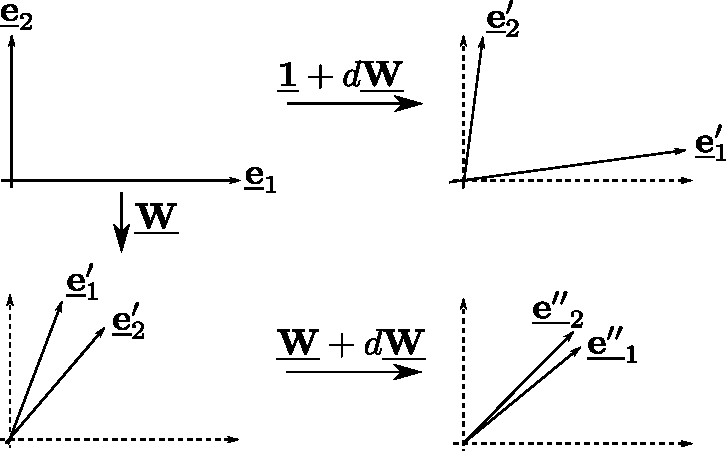
\includegraphics[width=10cm]{section2_fig18}  
  \caption{Illustration of gradient descent in transformed coordinate system}
  \label{fig:NatGrad}
\end{figure}
\begin{equation}
	d \vec{Z} = \underbrace{ d \vec{w} }_{ \text{then do } d \vec{w} }
	\cdot \underbrace{ \vec{w}^{-1} }_{ \substack{
		\text{transfer back to } \vec{1} \\
		\Rightarrow \text{ makes learning} \\
		\text{steps ''comparable''}} }
\end{equation}
This allows to do steepest ascent under normalized step size:
\\\\
Taylor-expansion of $e$ ($e^{(\alpha)}$ but $\alpha$ supressed in the
following):
\begin{eqnarray}
  e_{(\vec{w} + d \vec{w})} & = & e_{(\vec{w})} + \nabla e_{(\vec{w})}^T dw \\
  & = & e_{(\vec{w})} 
  + \underbrace{ \eta }_{ d \vec{w} = \eta \vec{z}_{\mathrm{w}} }
  \big[ \nabla e_{(\vec{w})} \big]^T \cdot \underbrace{ \vec{z}_{
      \mathrm{w}} }_{
     d\vec{w} = \eta \vec{z}_{\mathrm{w}} }
\end{eqnarray}
learning step:
\begin{equation}
	\begin{array}{ll}
		d \vec{Z} 
		& = d \vec{w} \cdot \vec{w}^{-1} \\\\
		& = \eta \vec{z}_{\mathrm{w}} \cdot \vec{w}^{-1}
	\end{array}
\end{equation}
direction of steepest ascent under normalized step-size:
\begin{equation}
	\big[ \nabla e_{(\vec{w})} \big]^T \vec{z}_{\mathrm{w}} 
	\eqexcl \max
\end{equation}
\begin{equation}
	\Big( \vec{z}_{\mathrm{w}} \cdot \vec{w}^{-1} \Big)^2 \eqexcl 1
\end{equation}
The solution for $z_{ij}$ can be found using Lagrange multipliers:
\begin{equation}
	\sum\limits_{i,j = 1}^N \frac{\partial e}{\partial \mathrm{w}_{ij}}
	\big( \vec{z}_{\mathrm{w}} \big)_{ij} - \lambda 
	\sum\limits_{i,j,k,l = 1}^N \big( \vec{z}_{\mathrm{w}} \big)_{ij}
	\big( \vec{w}^{-1} \big)_{jl} \big( \vec{z}_{\mathrm{w}} \big)_{ik}
	\big( \vec{w}^{-1} \big)_{kl} \eqexcl \max
\end{equation}
taking the derivative wrt.\ the $z_{\gamma,s}$ and setting to zero yields
\begin{equation}
	\frac{\partial e}{\partial w_{\gamma s}} - 2 \lambda
	\sum\limits_{k = 1}^N \big( \vec{z}_{\mathrm{w}} \big)_{\gamma k}
	\sum\limits_{l = 1}^N \big( \vec{w}^{-1} \big)_{kl} 
	\big( \vec{w}^{-1} \big)_{ls} \eqexcl 0
\end{equation}
\begin{equation}
	\frac{\partial e}{\partial \vec{w}} = 2 \lambda \vec{z}_{\mathrm{w}}
	\vec{w}^{-1} \big( \vec{w}^{-1} \big)^T
\end{equation}
\begin{equation}
	\vec{z}_{\mathrm{w}} = \frac{1}{2\lambda} \frac{\partial e}{\partial
		\vec{w}} \vec{w}^T \vec{w}
\end{equation}
yielding the direction for ''natural'' gradient ascent
\begin{equation}
	\Delta \vec{w} = \eta \frac{ \overbrace{\partial e}^{
		\substack{	\text{''original''} \\ 
				\text{gradient}} }}{\partial \vec{w}}
		\underbrace{ \vec{w}^T \vec{w} }_{
			\substack{	\text{normalization} \\
					\text{of step size}} }
\end{equation}
\begin{equation} \label{eq:natgrad2}
	\fbox{$ \Delta \mathrm{w}_{ij} = \eta \sum\limits_{l = 1}^N
	\left\{ \delta_{il} 
	+ \frac{ \widehat{f}_i^{''} \Big( \sum\limits_{k = 1}^N 
			\mathrm{w}_{ik} \mathrm{x}_k^{(\alpha)} \Big)
			}{\widehat{f}_i^{'} \Big( \sum\limits_{k = 1}^N 
			\mathrm{w}_{ik} \mathrm{x}_k^{(\alpha)} \Big)}
	\sum\limits_{k = 1}^N \mathrm{w}_{lk} \mathrm{x}_k^{(\alpha)}
	\right\} \mathrm{w}_{lj}
	$}
\end{equation}
\begin{itemize}
\item efficient \& fast learning rule (no matrix inversions
  necessary!)
\item this normalization of stepsize is equivalent to imposing a
  Riemannian metric (with metric tensor $\vec{G} = \vec{w}^{-1} \cdot
  \vec{w}^T$) on space of $\vec{w}$'s
\end{itemize}
% -----------------------------------------------------------------------------

\subsubsection{Some Practical Aspects}
\paragraph{(1) undetermined source amplitudes $\leadsto$ convergence problems}
\mbox{}\\\\
Bell-Sejnowski solution:
\begin{equation}
	\Delta \mathrm{w}_{ii} = 0 \text{ and } \mathrm{w}_{ii} = 1 
	\text{ for all } i
\end{equation}
Amari solution: Learning steps always orthogonal to subspace of
equivalent unmixing matrices.
\begin{equation}
	\Delta \mathrm{w}_{ij} = \eta \frac{ \widehat{f}_i^{''} \bigg( 
		\sum\limits_{k = 1}^N 
		\mathrm{w}_{ik} \mathrm{x}_k^{(\alpha)} \bigg)
		}{\widehat{f}_i^{'} \bigg( \sum\limits_{k = 1}^N 
		\mathrm{w}_{ik} \mathrm{x}_k^{(\alpha)} \bigg)}
		\sum\limits_{l \neq i}^N \Bigg( \sum\limits_{k = 1}^N
		\mathrm{w}_{lk} \mathrm{x}_k^{(\alpha)} \Bigg)
		\mathrm{w}_{lj}
\end{equation}

\paragraph{(2) choice of $\widehat{f}_i$ : true distribution is typically unknown} \mbox{} \\\\
Idea: probability density with one maximum is very likely $\leadsto$ cdf will be roughly sigmoidal
\\\\
typical choice:
\begin{equation} \tag{logistic function}
	\widehat{f}_{(y)} = \frac{1}{1 + \exp(-y)}
\end{equation}
\begin{equation}
	\frac{\widehat{f}_{(y)}^{''}}{\widehat{f}_{(y)}^{'}}
	= 1 - 2 \widehat{f}_{(y)}
\end{equation}
Observation: ICA is fairly robust against false choice of $\widehat{f}$. \\\\
Ansatz: Ignoring scaling of $\hat{s}_i$, i.e.\ using (\ref{eq:natgrad2}):
for stationary state of natural gradient ascent (batch) the following has to hold:
\begin{equation}
	\Delta \vec{w}_{ij} \eqexcl 0
\end{equation}
\begin{equation}
	\delta_{il} \eqexcl -\frac{1}{p} \sum\limits_{\alpha = 1}^p 
	\underbrace{ \frac{ \widehat{f}_i^{''} \bigg( 
		\sum\limits_{k = 1}^N 
		\mathrm{w}_{ik} \mathrm{x}_k^{(\alpha)} \bigg)
		}{\widehat{f}_i^{'} \bigg( \sum\limits_{k = 1}^N 
		\mathrm{w}_{ik} \mathrm{x}_k^{(\alpha)} \bigg)} }_{
			\varphi_i \big( \widehat{s}_i^{(\alpha)} \big) }
	\cdot \underbrace{ \sum\limits_{k = 1}^N \mathrm{w}_{lk} 
		\mathrm{x}_k^{(\alpha)} }_{
			\widehat{s}_l^{(\alpha)} }
\end{equation}
Ansatz: $\widehat{s}_i = \lambda_i s_i$ estimated $\sim$ true source signal\\\\
\indent $i = l$:
\begin{equation}
	-\frac{1}{p} \sum\limits_{\alpha = 1}^p \varphi_i \Big(
		\widehat{s}_i^{(\alpha)} \Big) \lambda_i s_i^{(\alpha)} 
		\eqexcl 1
\end{equation}
As $\lambda$ is a free parameter, this condition can always be fulfilled through proper choice of $\lambda_i$. \\\\
For $i \neq l$ and in the limit of large number of observations:
\begin{equation}
\delta_{il}	\frac{1}{p} \sum\limits_{\alpha = 1}^p \varphi_i \Big(
		\widehat{s}_i^{(\alpha)} \Big) \lambda_l s_l^{(\alpha)}
	\rightarrow \bigg< \varphi_i \Big(
		\widehat{s}_i^{(\alpha)} \Big) \lambda_l s_l^{(\alpha)}
		\bigg>_{P_{\vec{s}}}
\end{equation}
\begin{equation}
	\Big< \varphi_i \big( \lambda_i s_i \big) \lambda_l s_l \Big>
	\underbrace{ = }_{ \substack{ 	\text{statistical} \\
					\text{independence}} }
	\Big< \varphi_i \big( \lambda_i s_i \big) \Big>
	\Big< \lambda_l s_l \Big>
	\eqexcl 0
\end{equation}
Can always be fulfilled if data is ''centered'': $< s_l > = 0$
\\\\
Therefore true (independent) source signals are always a fixed point of the 
natural gradient ascent $\rightarrow$ independent of choice
of $\widehat{f}_i$

\begin{itemize}
	\itR however: if $\widehat{f}_i$ deviates too strongly from its true
		shape, the fixed point may become unstable
	\itR if in doubt (and enough data available)
	\begin{itemize}
		\itl make a parametrized ansatz for $\widehat{f}_i$
		\itl estimate parameters in addition to $\vec{w}$
	\end{itemize}
\end{itemize}

% -----------------------------------------------------------------------------
\newpage
\subsection{Second Order Blind Source Separation}

% -----------------------------------------------------------------------------

% \subsubsection{}
Compared to the estimation of correlations (second order moments), the
estimation of higher order moments from (small) samples of noisy
observations is often unreliable. In such cases, using
additional knowledge about the source signals can be exploited to
extend decorrelation methods and separate sources more robustly.

The following two methods (FFDIAG, QDIAG) exploit the assumption of
finite length \emph{autocorrelations} to implement noise robust
unmixing. Typical examples of such non-iid data displaying temporal
correlation structure include or time series such as videos, EEG, fMRI, MEG data.



\paragraph{2nd order ''separation'' idea:} find an unmixing matrix $\vec{w}$,
such that all cross-correlation functions vanish\footnote{All the
  presented approaches assume a \emph{linear} mixing model, i.e.\
  $\vec{x} \approx \vec{A} \vec{s}$. In many scenarios, this might not
  be a good model. However, for small amplitudes of variation around
  an operating point $\vec{s}_0$ this can still be used as a reasonable
  approximation for the more general relation $\vec{x} = f(\vec{s})$ as $\vec{x} =
  f(\vec{s}_1) = f(\vec{s_0 + \Delta s}) \approx f(\vec{s_0}) + \nabla f(\vec{s_0})  \Delta s$.}
\begin{center}
	statistical independence $\substack{ \text{?} 
		\\ \leftarrow
		\\ \Rightarrow }$ all cross-correlations vanish
\end{center}
\begin{figure}[h]
  \centering
  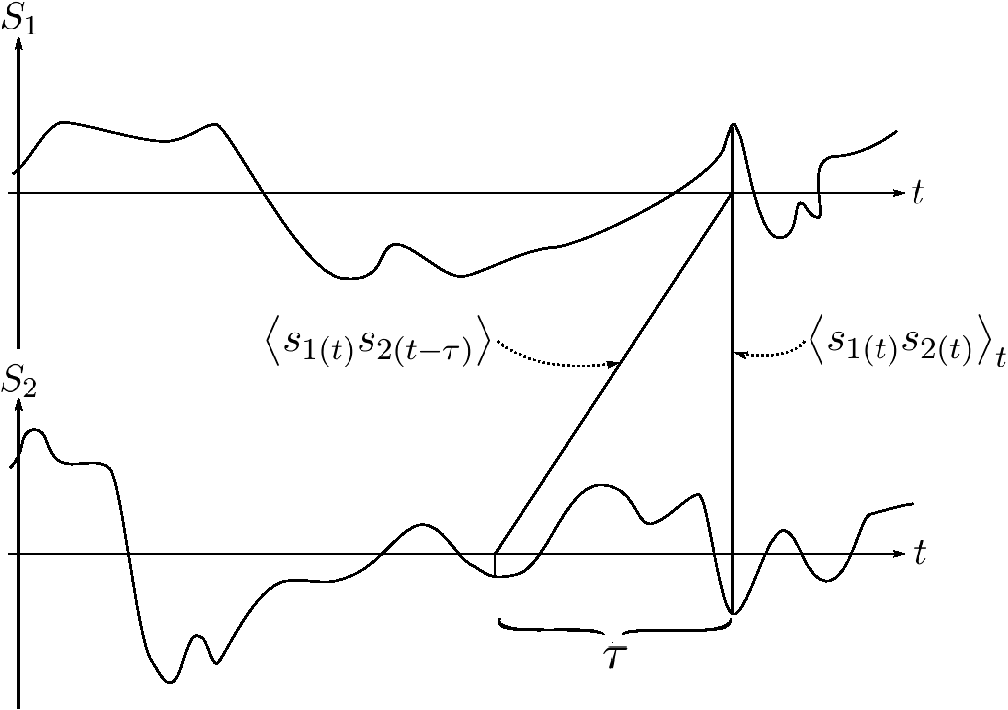
\includegraphics[width=10cm]{section2_fig19}  
  \caption{Source separation for time series data from two sources}
  \label{fig:timeSeriesICA}
\end{figure}


\paragraph{Example: Source separation using two shifts}\mbox{}\\
observations: $\vec{x}_{(t)}$, recorded at different times (from $\vec{x} = \vec{A} \vec{s}$)
\begin{enumerate}[(1)]
\item PCA and sphering
\begin{itemize}
	\itl ''centering'' of the data: $<\vec{x}> = \vec{0}$ \\
		usefull preprocessing for all ICA methods (often including
		dimension reduction)
	\itl solve the eigenvalue problem
	\begin{equation}
		\vec{C}_{\mathrm{x}}^{(0)} \vec{e}_k = \lambda_k \vec{e}_k
		\text{ with } \big[ \vec{C}_{\mathrm{x}}^{
			\overbrace{ (0) }^{ \tau = 0 } 
			} \big]_{ij}
		= \Big< \mathrm{x}_{i (t)} \mathrm{x}_{j (t)} \Big>_t
	\end{equation}
	\itl transformation into the eigenbasis and sphering
	\begin{equation}\label{sec:sphering}
		\vec{M}_0 = \underbrace{ \vec{\Lambda}_0^{-1} }_{
			\substack{	\text{diagonal matrix of} \\
					\text{inverse eigenvalues}} } \cdot
			\underbrace{ \vec{E}_0 }_{
				\substack{	\text{matrix of} \\
						\text{eigenvectors}} }
	\end{equation}
	\begin{equation}
		\vec{u} = \vec{M}_0 \vec{x}
	\end{equation}	
\end{itemize}
\item source separation requires one additional orthogonal transformation
\begin{itemize}
	\itl Ansatz: $\underbrace{ \vec{s} }_{ 
		\substack{ \text{true sources} \\ \text{(independent)}} }
		= \vec{B} \vec{u}$
	\itl for statistically independent sources we obtain
	\begin{equation}
		\begin{array}{lcl}
		\big< s_{i (t)} s_{j (t)} \big>_t 
		& \underbrace{ = }_{ \substack{	\text{statistical} \\
						\text{independence}} } 
				& \delta_{ij} \\\\
		& = & \sum\limits_{k,l = 1}^N B_{ik} \underbrace{
			\big< u_{k (t)} u_{l (t)} \big>_t }_{
				\substack{ \eqexcl \delta_{kl} \\
					\text{({\it cf. sphering})}} } 
			B_{lj}^T \\\\
		& = & \sum\limits_{k = 1}^N B_{ik} B_{kj}^T
		\end{array}
	\end{equation}
	\begin{equation}
		\vec{B} \cdot \vec{B}^T = \vec{1} \leadsto
		\text{orthogonal transformation}
	\end{equation}
\end{itemize}
\item determination of $\vec{B}$ through diagonalization of a time-shifted cross-correlation matrix
\begin{itemize}
	\itl solve the eigenvalue problem
	\begin{equation}
		\vec{C}_u^{(\tau)} \vec{e}_k = \lambda_k \vec{e}_k 
		\text{ with } \Big[ \vec{C}_u^{(\tau)} \Big]_{ij}
		= \Big< u_{i(t)} u_{j(t-\tau)} \Big>_t
	\end{equation}
	\itl transformation into the eigenbasis
	\begin{equation}\label{eq:EVshift}
		\widehat{\vec{s}} = \underbrace{\vec{E}_{  \tau }}_{
			\substack{ \text{matrix of} \\ \text{eigenvectors}} }
			\vec{u}
	\end{equation}
\end{itemize}
\end{enumerate}
\emph{Note:} The matrix of Eigenvectors is orthonormal
($\vec{E}^T_\tau\vec{E}_\tau=\vec{I}$) and therefore a candidate for $\vec{B}$. Combining equations (\ref{sec:sphering}) and (\ref{eq:EVshift}), this gives the transformation 
\begin{equation}
  \label{eq:2ndOrder}
\widehat{\vec{s}} = \vec{E}_\tau \vec{\Lambda}^{-1/2}_0 \vec{E}_0^T \vec{x}
\end{equation}

\paragraph{Noise robust algorithms in the general case:}
Given a set of $T$ zero-mean observations: $\vec{x}_{(t)}$ and corresponding 
number of $N$x$N$ covariance matrices indexed by $\tau$ 
\begin{equation}
	\Big[\vec{C}_{\mathrm{x}}^{(\tau)}\Big]_{ij} = 
	\frac{1}{T} \sum\limits_{t = 0}^{T-1} \mathrm{x}_{i(t)}
	\mathrm{x}_{j(t-\tau)}
\end{equation}
\begin{itemize}
	\item joint diagonalization of multiple cross-correlation matrices
	\item real world data: noise, approximate independence only
	$\leadsto$ only approximate diagonalization possible
	\item disturbances due to sensor noise can be minimized by ommitting $\tau = 0$
\end{itemize}
The following two algorithms implement these ideas using slightly different cost-functions. Both of them are implemented in the \texttt{jointDiag} package, available from CRAN.\footnote{\url{www.cran.r-project.org/web/packages/jointDiag/index.html}}

In order to find an $N \times N$ matrix $\vec{W}$ that diagonalizes the set of the matrices $\vec{C}^{(\tau)}, \tau = 0, 1, ...$ in a
least squares sense, we consider a cost function given by the squared sum of all off-diagonal elements
of $\vec{W} \vec{C}^{(\tau)} \vec{W}^T$. 


\begin{enumerate}[(1)]
\item QDIAG-algorithm
\\\\
\emph{cost function:} squared sum of non-diagonal elements:
\begin{equation}
	E_{[\vec{W}]}^T = \sum\limits_{\tau} \underbrace{ \alpha_\tau }_{
		\substack{ 	\text{weighting} \\ 
				\text{factors} \\
				\text{(optional)}} }
		\sum\limits_{i \neq j} \Big( \vec{W} \vec{C}_{\mathrm{x}}^{(\tau)} \vec{W}^T \Big)_{ij}^2
\end{equation}
\emph{optimization problem:}
\begin{equation}
	\begin{array}{rll}
		E_{[\vec{W}]}^T & \eqexcl \min 
		& \text{minimize cross-correlations} \\\\
		\Big( \vec{W} \vec{C}_{\mathrm{x}}^{(0)} \vec{W}^T \Big)_{ii}
			& = 1 \text{ for all } i
		& \text{avoid trivial solutions}
	\end{array}
\end{equation}
\emph{Comments:}
\begin{itemize}
\item \emph{documentation:} \textcite{VollgrafObermayer2006}, Matlab-code implementing the algorithm can be found on the NI-website\footnote{\url{www.ni.tu-berlin.de/menue/software/approximate_simultaneous_matrix_diagonalization_qdiag/}}
\item \emph{computational complexity:} two versions with complexity
	$O (k \cdot N^3)$ or $O (N^5)$
\item allows for arbitrary (rectangular) matrices $\vec{W}$
\end{itemize}

\item  FFDIAG-algorithm
\\\\
\emph{cost function:} equally weighted
\begin{equation}
	E_{[\vec{W}]}^T = \sum\limits_\tau \sum\limits_{i \neq j}
	\big( \vec{W} \vec{C}_{\mathrm{x}}^{(\tau)} \vec{W}^T \big)_{ij}^2
\end{equation}
\emph{optimization problem:}
\begin{equation}
	\begin{array}{ll}
		E_{[\vec{W}]}^T \eqexcl \min 
		& \text{minimize cross-correlation} \\\\
		\text{invertability of } \vec{W}
		& \text{to avoid trivial solutions}
	\end{array}
\end{equation}
\emph{Comments:}
\begin{itemize}
\item \emph{Documentation:} \textcite{ZieheEtAl2004} 
  \item computational complexity: $O (K \cdot N^2)$ (approaching $O (N^3)$ for large $N$) 
 requires square matrices $\vec{W}$, no weighting
\end{itemize}
\end{enumerate}
Preference for one or the other algorithm depends on problem size and kind of data (cf. \cite{StetterEtAl2000}), \slideref{Ex: optical imaging}

% -----------------------------------------------------------------------------

\subsection{Fast ICA}

\paragraph{ICA and Projection Pursuit}
''interesting'' complex features
\begin{itemize}
	\itl variance criterion $\Rightarrow$ PCA \\
		important preprocessing method, but: scale sensitive solutions
	\itl higher moments: ok, but: Why not maximize non-Gaussianity?
\end{itemize}
ICA and non-Gaussianity
\[ \begin{array}{lc}
	\vec{x} = \vec{A} \vec{s} 
	& \substack{ 	\text{mixing matrix } \vec{A} \text{, statistically} \\
		\text{independent sources}} \\\\
	\widehat{s}_i = \vec{w}_i^T \vec{x}
	& \substack{ 	\text{extraction of one source through one} \\
			\text{row vector of an unmixing matrix}} \\\\
	\widehat{s}_i = \underbrace{ \vec{w}_i^T \vec{A} }_{ \vec{z}_i^T }
		\vec{s} = \vec{z}_i^T \vec{s}
	& \substack{ 	\text{linear combination of statistically} \\
			\text{independent variables}}
\end{array} \]
''The sum of independent random variables is 'more Gaussian' then the original variables''
\begin{itemize}
	\itR interesting directions (projection pursuit) and individual 
		components (ICA) can be extracted by maximizing non-Gaussianity
		w.r.t $\vec{w}$
\end{itemize}

\paragraph{Measures for non-Gaussianity:} The Gaussian is fully characterized by its first and second moments. Deviations from Gaussianity can therefore be quantified via the following measures:
\begin{enumerate}[(1)]
\item Kurtosis
\begin{equation}
	\kurt(u) = \big< u^4 \big>_{P_u (u)} - 3 \underbrace{
		\Big( \big< u^2 \big>_{P_u (u)} \Big)^2 }_{
			\substack{	\text{would be } 1 \text{ for} \\
					\text{sphered data}}}
\end{equation}
\[ \begin{array}{lll}
	\kurt(u) = 0 & \text{Gaussian PDF} 
		& 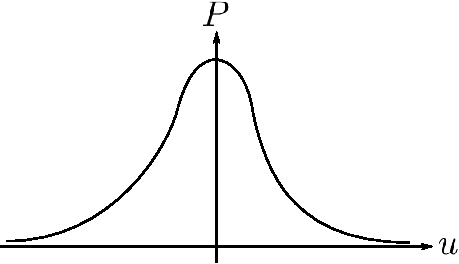
\includegraphics[width=4cm]{section2_fig20}
		\\\\
	\kurt(u) > 0 & \text{''super''-Gaussian PDF}		
		& 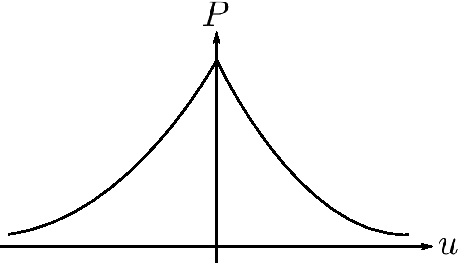
\includegraphics[width=4cm]{section2_fig21} \\
		& \rightarrow \text{ peaky, long tails (i.e. ''outliers'')} \\
		& \rightarrow \text{ e.g.: Laplace distribution} \\\\
	\kurt(u) < 0 & \text{''sub''-Gaussian PDF}
		& 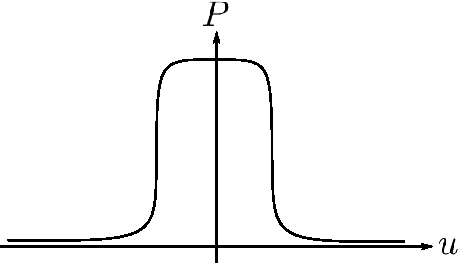
\includegraphics[width=4cm]{section2_fig22} \\
		& \rightarrow \text{ bulky, no ''outliers''} \\
		& \rightarrow \text{ e.g. constant distribution}
\end{array} \]
for independent random variables $u_1$ and $u_2$ we get:
\begin{equation}
	\begin{array}{rl}
		\kurt(u_1 + u_2) 
			& = \kurt(u_1) + \kurt(u_2) \\\\
		\kurt(z_1 u_1)
			& = z_1^4 \kurt(u_1)
	\end{array}
\end{equation}
\emph{Example:} two statistically independent sources with $\big< s_i s_j \big> = \delta_{ij}$
\begin{equation}
	\begin{array}{ll}
		\widehat{s} & = \vec{z}^T \vec{s} \\\\
			    & = z_1 s_1 + z_2 s_2
	\end{array}
\end{equation}
\begin{equation}
	\begin{array}{ll}
		\var(\widehat{s}) 
		& = \Big< \big( z_1 s_1 + z_2 s_2 \big)^2 \Big>_{P_s (s)} \\\\
		& = z_1^2 \big< s_1^2 \big> + z_2^2 \big< s_2^2 \big> \\\\
		& = z_1^2 + z_2^2
	\end{array}
\end{equation}
\begin{equation}
	\kurt(\widehat{s}) = z_1^4 \kurt(s_1) + z_2^4 \kurt(s_2)
\end{equation}
search for ''interesting'' directions
\begin{equation}
	\begin{array}{rllc}
	\kurt(\widehat{s}) & \eqexcl \max_{\vec{z}} 
	& \leftarrow & \substack{ 	\text{search for the direction} \\
					\text{of optimal kurtosis}} \\\\
	z_1^2 + z_2^2 & \eqexcl 1
	& \leftarrow & \substack{	\text{such that data} \\
					\text{remained sphered}}
	\end{array} 
\end{equation}
\emph{Result:} ({\it see supplementary material})
\begin{equation}
	\vec{z} = \left( \begin{array}{c}
			0 \\ \pm 1 
		\end{array} \right)
	\text{ or } 
	\vec{z} = \left( \begin{array}{c}
			\pm 1 \\ 0 
		\end{array} \right)
\end{equation}
independent sources correspond to extrema of the kurtosis
\item Negentropy
\begin{equation}
	J_{(u)} \coloneqq \underbrace{ H_{(u)}^{\mathrm{Gauss}} }_{
			\substack{ 	\text{entropy of Gaussian} \\
					\text{with variance } \sigma^2} }
		- \underbrace{ H_{(u)} }_{
			\substack{	\text{entropy of true} \\
					\text{distribution} \\
					\text{(variance } \sigma^2 \text{)} }}
\end{equation}
\begin{itemize}
	\item interesting, theoretically well founded measure
	\item but: hard to evaluate, optimization is computationally expensive (depends on full distribution)
\end{itemize}
\item Approximations to the negentropy
\begin{equation}
	J_{(u)} \approx \sum\limits_{i = 1}^l \underbrace{ k_i }_{
		\substack{	\text{some} \\ \text{constant}} }
		\bigg\{ \Big< G_{(u)} \Big>_{ \underbrace{ P_u (u) }_{
			\substack{ \text{true} \\ \text{density} } } }
		- \Big< G_{(u)} \Big>_{ \underbrace{ \mathrm{Gauss} }_{
			\substack{ 	\text{reference:} \\
					\text{Gaussian} \\
					\text{density with} \\
					\text{some variance}} } } \bigg\}
\end{equation}
common contrast functions:
\[ \begin{array}{lc}
	G_{1(u)} = \frac{1}{a} \log \cosh a u 
	& \substack{ 	\text{good general purpose function} } \\\\
	G_{2(u)} = -\exp \Big( -\frac{u^2}{2} \Big) 
	& \substack{	\text{good only if sources are} \\
			\text{highly ''super''-Gaussian} \\
			\text{i.e. many outliers} } \\\\
	G_{3(u)} = \frac{1}{4} u^4
	& \substack{	\text{kurtosis (see \textcircled{1}),} \\
			\text{useful if components} \\
			\text{are ''sub''-Gaussian} \\
			\text{i.e. few outliers}}
\end{array} \]
$\leadsto$ Clever choice of $G$ allows to obtain robust approximations to negentropy \textcite{Hyvaerinen1997}, \textcite{HyvaerinenOja2000}. 
\end{enumerate}

\paragraph{Fixed point algorithm for one linear neuron:}
The following algorithm (alg. \ref{alg:fastICA1}) implements \texttt{fastICA} for standardized data (mean=0, sd=1) to learn a single weight vector $\vec{w}$:
\[ \begin{array}{ll}
	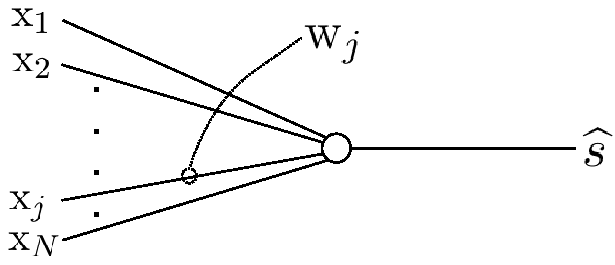
\includegraphics[width=6cm]{section2_fig23}
	& \widehat{s} = \underbrace{ \vec{w}^T }_{ 
		\substack{	\text{''interesting''} \\
				\text{complex} \\
				\text{features}} }
		\vec{x}
\end{array} \]
\begin{algorithm}
  \label{alg:fastICA1}
  \DontPrintSemicolon
  randomly initialize weight vector $\vec{w}$ of unit length\; 
  \Repeat{convergence}{
    \[ \begin{array}{ll}
	\vec{w}^+
	& = \frac{1}{p} \Bigg\{ \sum\limits_{\alpha = 1}^p \vec{x}^{(\alpha)}
		G_{\big( \vec{w}^T \vec{x}^{(\alpha)} \big)}^{'}
		-\vec{w} \sum\limits_{\alpha = 1}^p 
		G_{\big( \vec{w}^T \vec{x}^{(\alpha)} \big)}^{''}
		\Bigg\} \\\\
	\vec{w} 
	& = \frac{\vec{w}^+}{\|\vec{w}^+\|}
\end{array} \]
}
  \caption{fixed-point algorithm for fastICA: single component}
\end{algorithm}
\begin{itemize}
\item for details, see \textcite{Hyvaerinen1999} and \textcite[ch. 8.3.5]{HyvaerinenEtAl2001}.
	\item convergence to direction of extremal ''non-Gaussianity''
	\itR example of a so-called projection pursuit method
\end{itemize}

\paragraph{Fixed-point algorithm for a perceptron}
\[ \begin{array}{ll}
	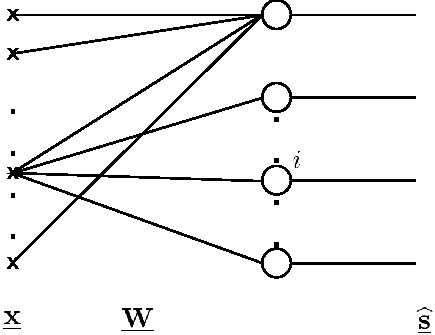
\includegraphics[width=6cm]{section2_fig24}
	& \widehat{\vec{s}} = \vec{W} \vec{x}
\end{array} \]
Algorithm \ref{alg:fastICAN} implements fastICA for standardized data (mean=0, sd=1) to learn the $N \times N$ weight matrix $\vec{W}$.
\begin{algorithm}
  \DontPrintSemicolon
  $t \leftarrow 0$\;
  randomly initialize weight vectors $\vec{w}_i^{(t)}\; \text{for } i \in 1 \dots N$\; 
\Repeat{convergence}{
   symmetric orthogonalization: 
%    $$
%    \vec{W}  \leftarrow \vec{W}/\lVert \vec{W} \rVert \qquad \text{(do not use frobenius norm)}
%    $$
    $$
    \vec{W}^{(t)}  \leftarrow  \frac{3}{2} \vec{W}^{(t)} 
    -  \frac{1}{2} \vec{W}^{(t)} \Big( \vec{W}^{(t)}
    \Big)^T \vec{W}^{(t)}
    $$
     \For{$i \in 1 \dots N$}{
    \begin{eqnarray*}
      \vec{w}_i^{(t)}
      & \leftarrow & \frac{1}{p} \left\{ \sum\limits_{\alpha = 1}^p \vec{x}^{(\alpha)}
        G^{'}\bigg( \big(\vec{w}_i^{(t)}\big)^T \vec{x}^{(\alpha)} \bigg)
        -\vec{w}_i^{(t)} \sum\limits_{\alpha = 1}^p 
        G^{''}\bigg( \big(\vec{w}_i^{(t)}\big)^T \vec{x}^{(\alpha)} \bigg)\right\}\\
      \vec{w}_i^{(t+1)} 	& \leftarrow & \frac{\vec{w}_i^{(t)}}{\| \vec{w}_i^{(t)} \|}
    \end{eqnarray*}
  }
    $t \leftarrow t+1$
  }
  \caption{fixed-point algorithm for fastICA: multiple components}
  \label{alg:fastICAN}
\end{algorithm}
\\\\
\emph{Remark:} The fastICA algorithm can be understood as a fixed point algorithm for maximum likelihood estimation of the ICA-model in which the learning rate for the different directions is adaptively adjusted (see \cite[p. 424]{HyvaerinenOja2000}). For further details, see \textcite[ch. 8.4]{HyvaerinenEtAl2001}. 
\\\\
\emph{code:} \url{http://research.ics.aalto.fi/ica}\\
\slideref{sound demo: blind source separation}
\slideref{natural images: van Hateren and van der Schaaf}

% -----------------------------------------------------------------------------
 %% Projection Methods
% ---------------------------- README -----------------------------------------
% This file holds section three of the body of the Machine Intelligence II 
% script.
% -----------------------------------------------------------------------------

\setcounter{equation}{0}
\newpage 
\section{Stochastic Optimization}
\label{sec:stochOptimization}
Most supervised and unsupervised learning problems involve
evaluation of a cost function $E^T$. For cost functions with
real-valued arguments, gradient based techniques allow to find
(locally) optimal solutions.

This chapter deals with methods to solve problems based on
cost-functions with \emph{discrete arguments} (e.g.\ cluster
assignment) where gradient-based techniques are not directly
applicable.

% -----------------------------------------------------------------------------

\subsection{Simulated Annealing}
Simulated annealing is a method for stochastic optimization and based on an
{analogy} to ''natural'' optimization. The optimisation algorithm
mimicks freezing or crystallization of a physical system during which
(not necessarily global) optima regarding the energy of the system are reached. The process involves
\emph{slow cooling} (glass vs. crystal $\Rightarrow$ annealing) via
a \emph{computational temperature} $T$ or ''noise parameter'' $\beta =
\frac{1}{T}$.
\\\\
%%%%%%%%%%%%%%%%%%%%%%%%%%%%%%%%%%%%%%%%%%%%%%%%%%%%%%%%%%%%%%%%%%%%%%%%%%%%%%
%% check formatting
%%%%%%%%%%%%%%%%%%%%%%%%%%%%%%%%%%%%%%%%%%%%%%%%%%%%%%%%%%%%%%%%%%%%%%%%%%%%%%
Given a set of \emph{discrete} variables: $\{s_i\}, i = 1, \ldots, N$ (with $s_i \in \mathcal{S}$) describing the \emph{state}\footnote{
we will use short-hand notation: $\vec{s}$ (''state'', but not necessarily a
  vector space)} of the system and a real-valued \emph{cost function}: 
\begin{equation}
	E: \vec{s} \mapsto E_{(\vec{s})} \in \mathbb{R}
\end{equation}
the \emph{goal} is to find the (globally) optimal state $\vec{s}^*$, such that 
\begin{equation}
	E \eqexcl \min 
\end{equation}
``\emph{Stochastic} simulated annealing'' (algorithm \ref{alg:simulatedAnnealing}) implements an iterative procedure to find this optimal state.
\begin{algorithm}[h]
  \DontPrintSemicolon
  initialization: $\vec{s}_0, \tau, M, \beta_0$ small ($\leadsto$ high $T$) \;
  \Begin(Annealing loop: $t=1,2,\dots$){ 
    $\vec{s}_t = \vec{s}_{t-1}$ (initialization of inner loop) \\
    \Begin(State Update loop: $M$ iterations){
      choose a new state $\vec{s}$ randomly (local to $\vec{s}_t$ -- e.g. bit flip)\;
      calculate difference in cost:  $\Delta E = E_{(\vec{s})}
      - E_{(\vec{s}_t)}$ \;
      switch $\vec{s}_t$ to $\vec{s}$ with probability $\mathrm{W}_{(\vec{s}_t \rightarrow \vec{s})} =  
      \frac{1}{1 + \exp( \beta_t \Delta E)}$\;
      (otherwise keep the old state $\vec{s}_t$) \;
      }
      $\beta_t = \tau \beta_{t-1}$  {\tiny (practical but theoretically not optimal)}
    }
    \label{alg:simulatedAnnealing}
    \caption{Stochastic simulated annealing}
  \end{algorithm}
\\
\emph{Remark:} $\vec{s}$ is often chosen ''similar'' or ''close'' to the old state, e.g.\ by randomly ''flipping'' one variable rather than sampling a completely random new state. 
\\\\
The dynamics of such a switching process are affected by the transition probability function $\mathrm{W}$ and its dependence on the temperature parameter $\beta$:
\begin{itemize}
\item transition probability $\mathrm{W}_{(\vec{s}_t \rightarrow \vec{s})}$ 
\begin{figure}[h]
  \centering
    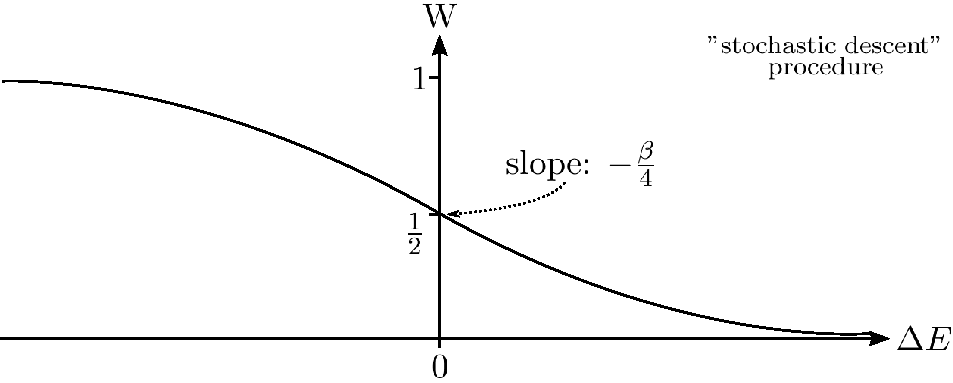
\includegraphics[width=9cm]{section3_fig1}
  \caption{Transition probabilities}
  \label{fig:transition}
\end{figure}
\item limiting cases

\begin{figure}[h] 
  \centering

  \begin{tabular}[h]{c c c}
$T \to \infty, \beta \to 0$ & & $T \to 0, \beta \to \infty$\\
high temperature & & low temperature \\
\begin{tikzpicture}[scale=2.25]
\draw[->] (-1,0) -- (1,0);
\draw[->] (0,0) -- (0,1.25);
\draw[lightgray, very thick] (-1,0.5) -- (.9,0.5);
\draw (0,0) node[anchor=north]{0};
\draw (0,1.25) node[anchor=west]{W};
\draw (1,0) node[anchor=west]{$\Delta E$};
\foreach \y in {0.5,1} \draw (0,\y) node[anchor=south east] {$\y$};
\foreach \y in {0.5,1} \draw (-1pt,\y) -- (1pt,\y);
\end{tikzpicture}
& &
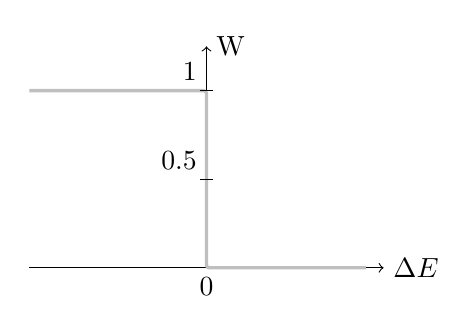
\begin{tikzpicture}[scale=2.25]
\draw[->] (-1,0) -- (1,0);
\draw[->] (0,0) -- (0,1.25);
\draw[lightgray, very thick, rounded corners=1pt](-1,1)-- (0,1) -- (0,0)--(0.9,0);
\draw (0,0) node[anchor=north]{0};
\draw (0,1.25) node[anchor=west]{W};
\draw (1,0) node[anchor=west]{$\Delta E$};
\foreach \y in {0.5,1} \draw (0,\y) node[anchor=south east] {$\y$};
\foreach \y in {0.5,1} \draw (-1pt,\y) -- (1pt,\y);
\end{tikzpicture}
  \end{tabular}
  \caption{Transition probabilities in the two limiting cases}
  \label{fig:transition}
\end{figure}
\end{itemize}
For many optimization problems, the cost function has local optima (see figure \ref{fig:localMinima}). 
\begin{figure}[h]
  \centering
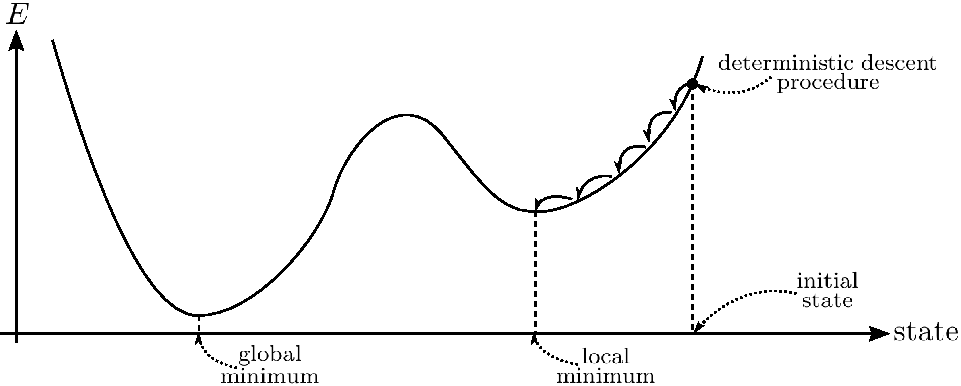
\includegraphics[width=12cm]{section3_fig3}  
  \caption{Cost function with local minima}
  \label{fig:localMinima}
\end{figure}
\begin{figure}[h]
  \centering
\[ \begin{array}{ccc}
	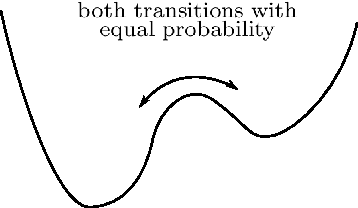
\includegraphics[width=4cm]{section3_fig4}
	& 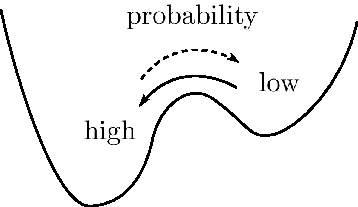
\includegraphics[width=4cm]{section3_fig5}
	& 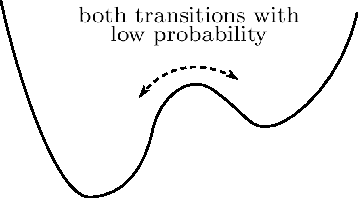
\includegraphics[width=4cm]{section3_fig6} \\\\
	\text{high } T, \text{ low } \beta 
	& \substack{	\text{intermediate values for} \\
			T \text{ and } \beta \\
			\Rightarrow \text{ escape from local} \\
			\text{optima is possible}}
	& \text{low } T, \text{ high } \beta
\end{array} \]
  
  \caption{Effect of annealing on local minima}
\end{figure}
In such cases, convergence to the global optimum of the cost function
is guaranteed if:
\begin{equation}
	\beta_t \sim \ln t
\end{equation}
\begin{itemize}
	\itR robust optimization procedure
	\itR but: $\beta_t \sim \ln t$ is too slow for practical problems
	\itR therefore: $\beta_{t+1} = \tau \beta_t, \tau = 1.01 \ldots 1.30$
		(exponential annealing)
	\itR additionally: the \texttt{State Update loop} has to be iterated often enough, e.g. $M=2000$ ($\leadsto$ thermal equilibrium), 
	however also $M=1$ can work if the temperature is decreased slowly enough
\end{itemize}

% -----------------------------------------------------------------------------

\newpage 						% for visual reasons
\subsection{The Gibbs Distribution}
The random (noisy) state changes cause state fluctuations even for
constant $T$ and $\beta$ (more precisely we have a stochastic process $\vec{s}_{t'}$ with the Markov property). Under certain conditions, these fluctuations
result in a \emph{stationary distribution} over all possible states,
where the probability of observing a specific state depends on its
energy (cost).
\\\\
$\Pi_{(\vec{s}, t')}$: probability distribution across states where $t'$ corresponds to the iteration 
count of the \texttt{State Update loop} of algorithm \ref{alg:simulatedAnnealing}.
\begin{equation}
	\Pi_{(\vec{s}, t')} \rightarrow 
	\underbrace{ P_{(\vec{s})} }_{ \substack{ 	\text{stationary} \\
							\text{distribution}} }
	\text{ for }
	t' \rightarrow \infty \text{ (and constant } T, \beta \text{)}
\end{equation}
calculation of $P_{(\vec{s})}$ under the assumption of "detailed balance" (reversible Markov process): 
\begin{equation}
	\underbrace{ \substack{	\text{probability of} \\
				\text{transition } 
				\vec{s} \rightarrow \vec{s}^{'}} }_{
			P_{(\vec{s})} \mathrm{W}_{(\vec{s} \rightarrow
				\vec{s}^{'})} }
	\underbrace{ = }_{ \substack{	\text{detailed} \\
					\text{balance}}}
	\underbrace{ \substack{	\text{probability of} \\
				\text{transition } 
				\vec{s}^{'} \rightarrow \vec{s} } }_{
			P_{(\vec{s}^{'})} \mathrm{W}_{(\vec{s}^{'} \rightarrow
				\vec{s})} }
\end{equation}
\begin{equation}
	\begin{array}{ll}
	\frac{P_{(\vec{s})}}{P_{(\vec{s}^{'})}}
	& = \frac{\mathrm{W}_{(\vec{s}^{'} \rightarrow \vec{s})}}{
		\mathrm{W}_{(\vec{s} \rightarrow \vec{s}^{'})}} \\\\
	& = \frac{1 + \exp\big\{ \beta \big( E_{(\vec{s})} - E_{(\vec{s}^{'})}
		\big) \big\} }{1 + \exp\big\{ \beta \big( E_{(\vec{s}^{'})} - 
		E_{(\vec{s})}\big) \big\} } \\\\
	& = \frac{1 + \exp( \beta \Delta E)}{1 + \exp( -\beta \Delta E)} \\\\
	& = \exp( \beta \Delta E) \frac{1 + \exp( -\beta \Delta E)}{
		1 + \exp( -\beta \Delta E) } \\\\
	& = \exp( \beta \Delta E )
	\end{array}
\end{equation}
this condition is fulfilled for:
\begin{equation} \tag{Gibbs-Boltzmann-distribution}
	P_{(\vec{s})} = \frac{1}{Z} \exp(-\beta E) 
\end{equation}
normalization constant / partition function (sum over all states):
\begin{equation}
	Z = \sum\limits_{\vec{s}} \exp(-\beta E)
\end{equation}
probability distribution depends on cost and temperature
\begin{figure}[h]
  \centering
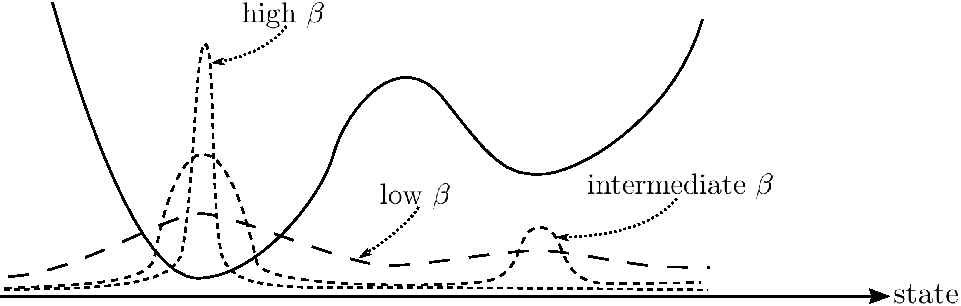
\includegraphics[width=12cm]{section3_fig7}  
\[ \begin{array}{ll}
	\beta \downarrow:
	& \text{broad, ''delocalized'' distribution} \\\\
	\beta \uparrow:
	& \text{distribution localized around (global) minima}
\end{array} \]
  \caption{cost-dependent probability distributions}
  \label{fig:costProba}
\end{figure}



% -----------------------------------------------------------------------------

\newpage						% for visual reasons
\subsection{Mean-Field Annealing}
\label{sec:mean-field-annealing}
Stochastic optimization can be computationally expensive: it depends on the cost function $E$ and the cooling schedule.\footnote{so far, we have left $E$ unspecified and -- in many cases -- it will be costly to compute} so a possible strategy might seem to evaluate $P_{(\vec{s})}$ directly ($P_{(\vec{s})}$ is known! -- the Gibbs-distribution). However: 
\begin{itemize}
	\item maxima of $P_{(\vec{s})}$ are equally hard to obtain as minima
		of $E$
	\item moments of $P_{(\vec{s})}$ can - in general - not be calculated
		analytically
\end{itemize}
Fortunately, a viable strategy is to approximate $P_{(\vec{s})}$ by a
computationally tractable distribution $Q_{(\vec{s})}$. 

\paragraph{Approximation:}\label{sec:fact-distr}
The distribution $Q_{(\vec{s})}$ to approximate $P_{(\vec{s})}$ is
chosen as a \emph{factorizing distribution} with costs $E_Q$ linear in
the state variable $\vec{s}$:
\begin{equation}
	Q_{(\vec{s})} \quad
= \quad \frac{1}{Z_Q} \exp \left\{ -\beta E_Q\right\} \quad
= \quad \frac{1}{Z_Q} \exp \Big\{ -\beta \sum\limits_{k}
		\underbrace{ e_k }_{ \text{parameters} } \mathrm{s}_k \Big\}
\end{equation}
\begin{itemize}
	\itr family of distributions parametrized by the \emph{mean fields} $e_k$
      \itr Goal: determine $e_k$ such that this approximation is as good as possible
\end{itemize}

\paragraph{Calculation of moments:}\label{sec:calculation-moments} More generally, moments of a distribution $P$ provide a concise description of $P$. For highly concentrated distributions (e.g.\ $\beta \to \infty$), the
1st moment (its \emph{mean}) gives a good characterization of the distribution
(e.g.\ if it is highly peaked also for the location of its maximum). For the factorizing distribution $Q_{(\vec{s})}$,
these moments can be calculated easily:
\begin{equation}\label{eq:factorizingMoments}
	\Big< f_{(\vec{s}/s_l)} g_{(s_l)} \Big>_Q
	 = \frac{1}{Z_Q} \sum\limits_{\vec{s}} f_{(\vec{s}/s_l)}
		g_{(s_l)} \exp \Big\{ -\beta \sum\limits_k e_k s_k \Big\}
\end{equation}
\begin{eqnarray*}
	& = & \frac{1}{Z_Q} \Bigg[ \sum\limits_{\vec{s}/s_l} f_{(\vec{s}/s_l)}
		\exp \Big( -\beta \sum\limits_{k \neq l} e_k s_k \Big) \Bigg]
		\Bigg[ \sum\limits_{s_l} g_{(s_l)} \exp \Big( -\beta e_l
			s_l \Big) \Bigg] \\\\
	& = & \frac{1}{Z_Q} \Bigg[ \sum\limits_{\vec{s}/s_l} f_{(\vec{s}/s_l)}
		\exp \Big( -\beta \sum\limits_{k \neq l} e_k s_k \Big) \Bigg]
  \frac{\sum\limits_{s_l} \exp(-\beta e_l s_l)}{\sum\limits_{s_l}
		\exp(-\beta e_l s_l)}
		\Bigg[ \sum\limits_{s_l} g_{(s_l)} \exp \Big( -\beta e_l
			s_l \Big) \Bigg] \\\\
	& = &\Big< f_{(\vec{s}/s_l)} \Big>_Q \frac{\sum\limits_{s_l}
		g_{(s_l)} \exp(-\beta e_l s_l)}{\sum\limits_{s_l}
		\exp(-\beta e_l s_l)} \\\\
	& = & \underbrace{ \Big< f_{(\vec{s}/s_l)} \Big>_Q \cdot \Big<g_{(s_l)} 
		\Big>_Q }_{ 	\substack{ \text{factorization of moments} \\
				\rightarrow \text{uncorrelated variables}} }
\end{eqnarray*}
\\
The first moments $\big< s_l \big>_Q$ play a central role in the approximation of $P$ by $Q$ (see below) and usually have a tractable expression:  
% E.g. for $\mathcal{s} = \{0,1\}$  
\begin{equation} \label{eq:mfa_firstmoment_Q}
	\big< s_l \big>_Q = \frac{\sum\limits_{s_l \in \mathcal{S}} s_l \exp(-\beta e_l s_l)}{
					\sum\limits_{s_l \in \mathcal{S}} \exp(-\beta e_l s_l)}
\end{equation}

\paragraph{The mean-field approximation:}
\begin{equation}
	\begin{array}{llc}
	P_{(\vec{s})} 
	& = \frac{1}{Z_p} \exp(-\beta E_p) 
	& \substack{ \text{true distribution} } \\
	Q_{(\vec{s})} 
	& = \frac{1}{Z_Q} \exp\big(-\beta \overbrace{\sum\limits_k e_k s_k}^{E_Q} \big)
	& \substack{ \text{approximation: family of} \\ \text{factorizing distributions} } \\\\
	e_k:
	& \text{\textit{mean fields} }
	& \substack{ \text{parameters to} \\ \text{be determined} }
	\end{array}
\end{equation}
minimization of the KL-divergence:
\begin{equation}
	\dkl(Q||P) = \sum\limits_{\vec{s}} Q_{(\vec{s})} \ln \frac{Q_{(\vec{s})}}{
		P_{(\vec{s})}} \eqexcl \min_{\vec{e}}
\end{equation}
\begin{equation}
	\begin{array}{ll}
	\frac{\partial}{\partial e_l}\dkl
	& = \frac{\partial}{\partial e_l} \bigg\{ \beta \sum\limits_{\vec{s}}
		Q_{(\vec{s})} E_p - \beta \sum\limits_{\vec{s}} 
		Q_{(\vec{s})} E_Q + \ln Z_p - \ln Z_Q \bigg\} \\\\
	& = \beta \frac{\partial}{\partial e_l}\big< E_p \big>_Q
		\underbrace{ -\beta \frac{\partial}{\partial e_l} 
			\sum\limits_{\vec{s}} Q_{(\vec{s})} \sum\limits_k
			e_k s_k }_{ -\beta \sum\limits_k e_k
                        \frac{\partial}{\partial e_l}\big< s_k \big>_Q - \beta
			\big< s_l \big>_Q }
		\underbrace{ -\frac{1}{Z_Q} \sum\limits_{\vec{s}} 
			\frac{\partial}{\partial e_l} \exp(-\beta
			\sum\limits_k e_k s_k) }_{ +\beta \big<s_l\big>_Q }
			\\\\
	& = \beta \frac{\partial}{\partial e_l}\big< E_p \big>_Q -\beta \sum\limits_k 
                        e_k \frac{\partial}{\partial e_l}\big< s_k \big>_Q 
 \qquad \eqexcl \qquad 0
	\end{array}
\end{equation}
The solution to this equation determines the mean fields $e_k$
minimzing $\dkl$ and depends on the exact form of $E_p$. It can be
found by solving the equations:
\begin{equation}\label{eq:MeanfieldEquation}
	\fbox{$ \frac{\partial}{\partial e_l}\big<E_p\big>_Q 
		- \sum\limits_k e_k \frac{\partial}{\partial e_l} \big<s_k\big>_Q = 0
	$}
\end{equation}
The latter simplifies further to 
\begin{equation} \label{eq:mfa_meanfields_simplified}
\fbox{$ \frac{\partial}{\partial e_l}\big<E_p\big>_Q 
		- e_l \frac{\partial}{\partial e_l} \big<s_l\big>_Q = 0
	$}
\end{equation}

because of the independent $\{s_k\}$  under the factorizing distribution $Q$.

\begin{algorithm}[h]
  \DontPrintSemicolon
  initialization: $\langle \vec{s} \rangle_0, \beta_0, t = 0$ \;
  \Begin(Annealing loop){ 
    \Repeat{$|e_k^\mathrm{old}-e_k^\mathrm{new}| < \varepsilon$}
    {
      calculate mean-fields: $e_k, \ \ k = 1, \ldots, N$ \;
      calculate moments: $\big<s_k\big>_Q,\ \ k = 1, \ldots, N$ \;
    }
    increase $\beta$ \;
    }
    \label{alg:MeanFieldAnnealing}
    \caption{Mean Field Annealing}
  \end{algorithm}

\begin{itemize}
	\itR inner loop: fixed-point iteration  for the mean-fields $e_k$
	\itR the moments $\big< s_k \big>$ for not too small temperatures are in general not from the discrete set $\mathcal{S}$ 
	  but range continuously between the elements of $\mathcal{S}$ 
	\itR however: $\beta \rightarrow \infty (T \rightarrow 0): \big< s_k \big>
		\rightarrow s_k^{*}$ \\
		because $P_{(\vec{s})}$ becomes singular at the state 
		$\vec{s}^*$ of minimal cost!
	\itR deterministic (fast) rather than stochastic (slow) optimization
		method (given that mean-field equations can be easily evaluated)
\end{itemize}

see \textcite{BilbroEtAl1989} and \textcite{Rose1998} for details. 
\\

\paragraph{Example (based on Ising model):}
Consider the quadratic cost function $E(s_1, \dots, s_N)$ for binary state vectors, i.e., $s_k \in \mathcal{S} = \{+1, -1\}$,
\begin{equation}
 E_p(\vec{s}) = -\frac{1}{2} \sum\limits_{\substack{i=1,j=1 \\ i\ne j}}^N W_{ij} s_i s_j,
\end{equation}
with a real symmetric matrix $\vec{W}$ with zeros on the diagonal ($\to$ no self-coupling).

The expressions required for the algorithm \ref{alg:MeanFieldAnnealing} can be directly
calculated: 
\begin{enumerate}
 \item The first moment, cf. eq. \eqref{eq:mfa_firstmoment_Q}, become: 
    \begin{align} 
      \big< s_k \big>_Q &= \frac{\sum\limits_{s_k \in \mathcal{S}} s_k \exp(-\beta e_k s_k)}{
					\sum\limits_{s_k \in \mathcal{S}} \exp(-\beta e_k s_k)} \\
			&= \frac{+1 \exp(-\beta e_k) -1 \exp(\beta e_k)}{\exp(-\beta e_k) + \exp(\beta e_k)} \nonumber \\
			&= \tanh(-\beta e_k) \nonumber
    \end{align}
 \item The mean-fields, cf. eq. \eqref{eq:mfa_meanfields_simplified}, are given by 
  \begin{align}
    0 &= \frac{\partial}{\partial e_k}\langle E_p\rangle _Q 
		- e_k \frac{\partial}{\partial e_k} \langle s_k\rangle _Q \\
     &= \frac{\partial}{\partial e_k}\left \langle -\frac{1}{2} 
	  \sum\limits_{\substack{i=1,j=1 \\ i\ne j}}^N W_{ij} s_i s_j \right \rangle_{\substack{Q \\ {} \\ {} \\ {}}} 
		- e_k \frac{\partial}{\partial e_k} \langle s_k\rangle_Q \nonumber \\
     &=  -\frac{1}{2} 
	  \frac{\partial}{\partial e_k} \sum\limits_{\substack{i=1,j=1 \\ i\ne j}}^N W_{ij} \langle s_i \rangle_Q \langle s_j \rangle_Q 
		- e_k \frac{\partial}{\partial e_k} \langle s_k \rangle_Q \nonumber \\
     &= -  \sum\limits_{\substack{i=1 \\ i\ne k}}^N W_{ik} \langle s_i \rangle_Q \frac{\partial}{\partial e_k} \langle s_k \rangle_Q 
		- e_k \frac{\partial}{\partial e_k} \langle s_k\rangle _Q \nonumber
  \end{align}
  which implies
  \begin{equation}
   e_k = -  \sum\limits_{\substack{i=1 \\ i\ne k}}^N W_{ik} \langle s_i \rangle_Q.
  \end{equation}

  Remark: the fixed-point iteration for the mean-fields $\vec{e}$ of this example converges (locally)
  which can be proven
%   \footnote{show: upper bounding the largest eigenvalue of the iteration function's jacobian (having elements
%  with the frobenius norm and show that it remains between $[0,1)$ 
%   i.e., that the iteration 
%   fuction is a contraction} 
using the 
  Banach fixed point theorem (at least for sufficiently large $\beta$).
\end{enumerate}


% -----------------------------------------------------------------------------
 %% Stochastic Optimization
% ---------------------------- README -----------------------------------------
% This file holds section four of the body of the Machine Intelligence II 
% script.
% -----------------------------------------------------------------------------

\setcounter{equation}{0}
\newpage 
\section{Clustering and Embedding}

While projection methods search for interesting directions / features
along which data differ, clustering methods yield groupings of the
data according to a specified similarity or distance measure.

While methods of central clustering typically also find
representatives (e.g.\ group averages or prototypes) for these different groups,
\emph{pairwise clustering} methods just need estimates of distances
(e.g. similiarity judgements) between pairs of data points. 
% -----------------------------------------------------------------------------

\subsection{K-means Clustering}

% -----------------------------------------------------------------------------

\subsubsection{The Clustering Problem}
\paragraph{Goal:} partitioning of observations 
$\vec{x}^{(\alpha)}, \alpha = 1, \ldots, p; \vec{x}^{(\alpha)} \in \mathbb{R}^N$
according to similarity. This is illustrated in figure \ref{fig:clusteringProblem}. 
\begin{figure}[h!]
  \centering
  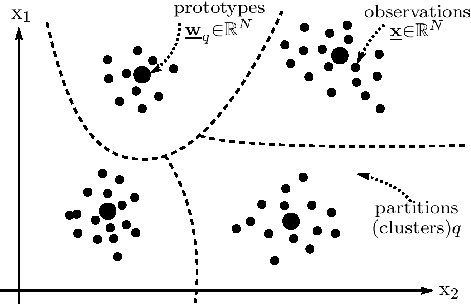
\includegraphics[width=10cm]{section4_fig1}  
  \caption{The clustering problem}
  \label{fig:clusteringProblem}
\end{figure}

\begin{itemize}
	\itR unsupervised formation of categories (partitions, clusters) 
		according to predefined criteria
	\itR description of clusters by prototypes $\leftarrow$ ''central'' 
		clustering
\end{itemize}


\paragraph{K-means Clustering:} ``prototype-based clustering''
\label{sec:kmeans}
\begin{itemize}
\item based on average quadratic Euclidean distance between observations and prototypes
\item simple \& most common procedure for clustering of vectorial data
\end{itemize}
\textbf{Cluster model:}\\\\
prototypes: $\vec{w}_q, q = 1, \ldots, M$ \qquad\qquad (M: number of clusters)
\\\\
binary assignment variables $m_q^{\alpha}$:
\begin{equation}
	m_q^{(\alpha)} = \left\{ \begin{array}{ll}
		1, & \text{if } \vec{x}^{(\alpha)} \text{ belongs to cluster } q
		\\\\
		0, & \text{else}
	\end{array} \right. 
\end{equation}
normalization:
\begin{equation}
	\sum\limits_q m_q^{(\alpha)} = 1
\end{equation}
cost function (''empirical risk''):
\begin{equation}\label{eq:euclideanClusterCost}
	E_{ \big[ \big\{ m_q^{(\alpha)} \big\}, \big\{ \vec{w}_q \big\} 
		\big] }^T = \frac{1}{2p} \sum\limits_{q,\alpha} m_q^{(\alpha)}
		\big( \vec{x}^{(\alpha)} - \vec{w}_q \big)^2
\end{equation}
The cost function represents the average quadratic distance between
observations and prototypes (''variance''). The choice of
similarity/distance measure should be based on prior knowledge (if available). 

Remark: If $\vec{w}_q$ is center of mass $\implies$ $E^T = \frac{1}{2} \cdot \mathrm{variance}$.
\\\\
model selection:
\begin{equation}
	E^T \eqexcl \min \leftarrow \substack{	\text{continous/discrete} \\
						\text{optimization problem}}
\end{equation}
\[ \text{validation} \left\{ \begin{array}{c}
	\substack{	\text{no, if goal is ''just'' to} \\
			\text{describe the set of observations}} \\\\
	\substack{	\text{yes, if goal is inference/prediction} \\
			\text{on future observations (e.g. calculating} \\
			m_q^{(\mathrm{new})} \text{ for a new observation }
			\vec{x}^{(\mathrm{new})} \text{)}}
\end{array} \right. \]
The computations involved in the cost function for k-means clustering are illustrated in figure \ref{fig:kMeansCostfunction}. 
\begin{figure}[h!]
  \centering
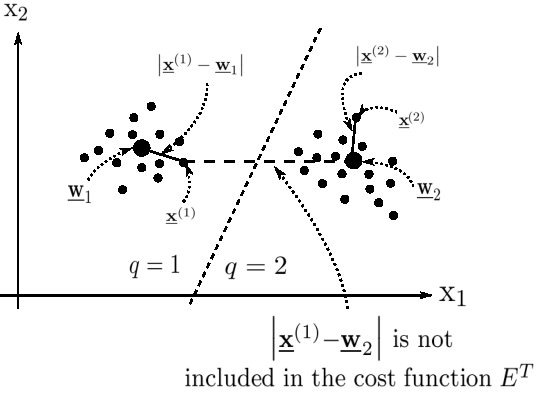
\includegraphics[width=10cm]{section4_fig2}  
  \caption{Illustration of the k-means cost function}
  \label{fig:kMeansCostfunction}
\end{figure}



% -----------------------------------------------------------------------------

\subsubsection{Model Selection}
\label{kmeans_modelselection}
Optimization problem with continuous (cluster-centers) and discrete
(cluster-assignment: binary) variables. Dissimilarity measure is Euclidean distance. 
\begin{itemize}
	\itR two step descent procedure (algorithm \ref{alg:batch-k-means})
\end{itemize}
\begin{algorithm}[h!]
\DontPrintSemicolon
  randomly initialize prototypes e.g.\ around (i.e., +noise) the whole data's center of mass, e.g., using PCA for spread quantification\;
  \Begin(loop){
  (1) choose  $m_q^{(\alpha)}$ ... \;
... such that $E^T$ is minimal for the given prototypes\;
\[ m_q^{(\alpha)} \left\{ \begin{array}{ll}
	1, & \text{if } q = \argmin_{\gamma} \big| \vec{x}^{(\alpha)}
		- \vec{w}_{\gamma} \big| \\
	0, & \text{else}
\end{array} \right. \]
$\Rightarrow$ assign every data point to its nearest prototype \;
\;
(2) choose  $\vec{w}_q$ ...\;
... such that $E^T$ is minimal for the -new- assignments\;
\[ \vec{w}_q = \frac{\sum\limits_{\alpha} m_q^{(\alpha)} \vec{x}^{(\alpha)}}{
	\sum\limits_{\alpha} m_q^{(\alpha)}}
\]
$\Rightarrow$ set $\vec{w}_q$ to the center of mass of its assigned data
}
    \label{alg:batch-k-means}
    \caption{batch k-means}
\end{algorithm}

\paragraph{center of mass is optimal:} condition for extremal point:
\begin{equation}
	\begin{array}{ll}
	\frac{\partial}{\partial \vec{w}_q} \bigg\{ \frac{1}{2p} 
	\sum\limits_{q^{'}, \alpha} m_{q^{'}}^{(\alpha)} 
	\big( \vec{x}^{(\alpha)} - \vec{w}_{q^{'}} \big)^2 \bigg\}
	& = -\frac{1}{p} \sum\limits_{\alpha} m_q^{(\alpha)} 
		\big( \vec{x}^{(\alpha)} - \vec{w}_q \big) \eqexcl 0 \\\\
	& \leadsto \vec{w}_q = \frac{\sum\limits_{\alpha} m_q^{(\alpha)}
		\vec{x}^{(\alpha)}}{\sum\limits_{\alpha} m_q^{(\alpha)}}
	\end{array}
\end{equation}
condition for minimum:
\begin{equation}
	\begin{array}{ll}
	\frac{\partial^2}{\partial \mathrm{w}_{qi} \partial \mathrm{w}_{
		q^{''}j}} \bigg\{ \frac{1}{2p} \sum\limits_{q^{'}, \alpha}
		m_{q^{'}}^{(\alpha)} \big( \vec{x}^{(\alpha)} - \vec{w}_{q^{'}}
		\big)^2 \bigg\} 
	& = \frac{\partial}{\partial \mathrm{w}_{q^{''}j}} \bigg\{
		-\frac{1}{p} \sum\limits_{\alpha} m_q^{(\alpha)} 
		\big( \mathrm{x}_i^{(\alpha)} - \vec{w}_{qi}
		\big) \bigg\} \\\\
	& = \Big( \frac{1}{p} \sum\limits_{\alpha} m_q^{(\alpha)} \Big)
		\delta_{ij} \delta_{qq^{''}}
	\end{array}
\end{equation}
\begin{itemize}
	\itl diagonal matrix with all positive entries
	\itl condition for minimum always fulfilled
\end{itemize}
\begin{itemize}
\item $E^T$ is non-increasing in every step and $E^T$ is bounded from below $\Rightarrow$ K-means clustering converges to a (local) optimum of $E^T$. 
\item $E^T$ at the solution can be interpreted as the average variability
within the groups.
\end{itemize}
\begin{figure}[h!]
  \centering
  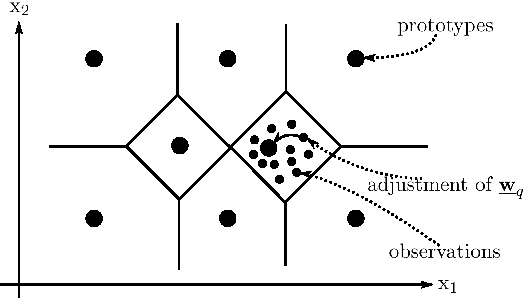
\includegraphics[width=9cm]{section4_fig3}  
  \caption{k-means and tesselation}
  \label{fig:tesselation}
\end{figure}


tesselation cell: region of data space for which
\begin{equation}
	q = \argmin_{\gamma} \big| \vec{x} - \vec{w}_{\gamma} \big|
\end{equation}
This interpretation is illustrated in figure \ref{fig:tesselation} and provides an alternative 2-step interpretation of k-means clustering
in terms of an optimized tesselation of the input-space:
\begin{enumerate}[(1)]
\item construct tesselation of feature space
\item adjust prototypes to the center of mass of all data points 
		within the corresponding tesselation cell
\end{enumerate}

\paragraph{''on-line'' version of K-means Clustering:}
The k-means procedure can be implemented in an on-line fashion (algorithm \ref{alg:on-line-k-means}) that is often more robust wrt.\ local minima than batch-learning and can be useful for streaming-data. 
\begin{algorithm}[h]
  \DontPrintSemicolon
  initialize prototypes e.g.\ around center of mass \;
  select learning step  $0 < \eta << 1$\;
  \Begin(loop){
    choose a data point $\vec{x}^{(\alpha)}$ \;
    assign data point to its closest prototype $q$\;
    \[ q = \argmin_{\gamma} \big| \vec{x}^{(\alpha)} - \vec{w}_{\gamma} \big| \]
    change corresponding prototype according to\;
    \[ \Delta \vec{w}_q = \eta \big( \vec{x}^{(\alpha)} - \vec{w}_{\gamma} \big) \]
    change $\eta$ \;
  }
  \label{alg:on-line-k-means}
  \caption{on-line k-means}
\end{algorithm}
\\
Goodness of the found solution depends on choosing an appropriate ''annealing'' schedule for $\eta$: Robbins-Monro conditions ({\it cf. MI I, section 1.4.1}). A typical schedule is shown in figure \ref{fig:annealingScheduleKMeans}. 
\begin{figure}[h!]
  \centering
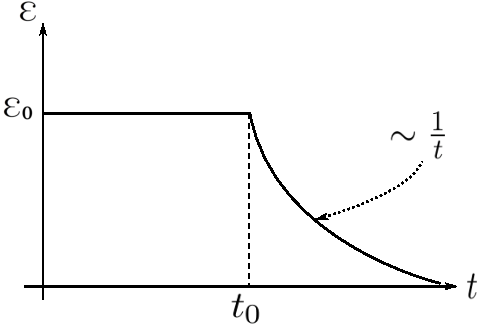
\includegraphics[height=5cm]{section4_fig4} 
  \caption{Annealing schedule ($t$ is the number of iterations)}
  \label{fig:annealingScheduleKMeans}
\end{figure}



% -----------------------------------------------------------------------------

\subsubsection{Number of Prototypes}
The number of prototypes is a hyperparameter of k-means clustering. Knowledge about the data (noise amplitude) and robustness of the clustering solution can guide this choice. 

\paragraph{choice of resolution}
\[ \begin{array}{ll}
	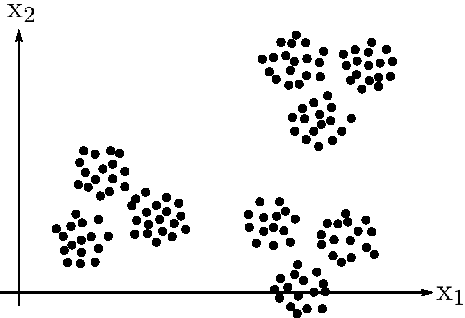
\includegraphics[width=6cm]{section4_fig5}
	& \begin{array}{l}
		\text{1 cluster} \\
		\text{3 cluster} \\
		\text{9 cluster} \\
		\text{many cluster?} \\\\
		\Rightarrow \substack{	\text{additional prior} \\
					\text{knowledge is needed!}}
	\end{array}
\end{array} \]
$E_{\min}^T$: average size of cluster (in terms of variance)
\begin{itemize}
	\itl large for few clusters -- small for many clusters
	\itl zero, if number of cluster $\corresponds$ number of data points
\end{itemize}
Note that $E^T_\mathrm{min}$ goes down if $M$ increases.
\\

The choice of resolution should depend prior knowledge on the average
size of the cluster (e.g.\ clusters ``smaller'' than the variance of noise probably do not capture meaningful structure). 
\begin{itemize}
	\itr exploit prior knowledge on $E_{\min}^T$ 
        (e.g.\ $E_{\min}^T \geq \sigma_\mathrm{noise}^2$ which is a natural boundary on 
        $E^T_\mathrm{min}$ )
\end{itemize}
This prior knowledge can be exploited using the heuristic of
\emph{iterative refinement}, as illustrated in algorithm \ref{alg:iterative-k-means-refinement}.

\begin{algorithm}
\DontPrintSemicolon
initialization: $\vec{w}_1 = \frac{1}{p} \sum\limits_{\alpha} 
	\vec{x}^{(\alpha)}, \underbrace{ \big( E_{\min}^T \big)^* }_{
			\substack{	\text{desired minimal} \\
					\text{average variance}} }
		, M = 1$ \;
\Begin(loop){
\lIf{$E_{\min}^T < \big( E_{\min}^T \big)^*$}{STOP} \;
select partition $q \in \{ 1, \ldots, M \}$ with largest variance
\[ q = \argmax_{\gamma} \left( \frac{\sum\limits_{\alpha} m_\gamma^{(\alpha)}
  \big( \vec{x}^{(\alpha)} - \vec{w}_\gamma \big)^2}{\sum\limits_{\alpha}
  m_\gamma^{(\alpha)}} \right) \]
add a new prototype:  $\vec{w}_{M+1} = \vec{w}_q + 
\underbrace{ \vec{\eta}_q }_{ \substack{	\text{small random} \\
    \text{vector}} }$\;
$M \leftarrow M + 1$\\
do k-means clustering with these $M$ prototypes \\
}
\label{alg:iterative-k-means-refinement}
\caption{iterative k-means refinement}
\end{algorithm}

\paragraph{Robustness of clustering solution}\mbox{}\\\\
\emph{Idea:} If the solution captures meaningful structure in the
data, multiple runs of the same algorithm with different initial
conditions should yield similar solutions.
\\\\
\emph{Caveat:} Assignment of labels to clusters is arbitrary: permutation of labels does
neither change cost nor character of the solution. 
\[ \begin{array}{l}
	1, 2, 3, \ldots, M \\
	9, 1, M, \ldots, 7
      \end{array} 
\]
This ``permutation symmetry''leads to $M!$ trivially equivalent optima, so the robustness-criterion needs to account for such equivalence classes of optima.  
The number of equivalence class increases with increasing number of prototypes
$\leadsto$ structurally different equivalent classes to be compared!


How many prototypes? $\rightarrow$ increase number until
''overfitting'' occurs
\begin{itemize}
  \itl many equivalence classes with approximately equal cost
  \itl different initial conditions and different sequences of pattern 
  presentation lead to clustering solutions from different 
  equivalence classes
  \itl different sub-datasets lead to solutions from different 
  equivalence classes
\end{itemize} 

\paragraph{Validation measure}\mbox{}\\\\
\textcite{LangeEtAl2004} estimate expected dissimilarity between
solutions for different samples from the same dataset $\leadsto$
``best'' number of clusters yields most robust clustering (highest
similiarity). For further details, see \textcite{Luxburg2010}. 
\begin{itemize}
\item Model free approaches:  Stability based validation
\item \textbf{Idea:} taking to many or too few clusters leads to unstable partitions
\item $\mathbf{X} = \big\{ \vec{x}^{(\alpha)} \big\}, \alpha = 1, \ldots, p; \quad \vec{x} \in \mathbb{R}^N$ ;\
A solution of the clustering algorithm is $\mathbf{Y} =(y_{1}, \ldots , y_{p})$ where $y_{i} \in L:=\{1,\ldots,M\}$
\item Comparing clustering solutions $Y_{1}$ and $Y_{2}$:\\
$$d:= \frac{1}{|\mathbf{Y_1}|}
      \sum_\alpha \mathbf{1}\left\{Y_{1, \alpha}\neq Y_{2, \alpha} \right\}\qquad$$ 
\end{itemize}
\begin{algorithm}
\DontPrintSemicolon
\Begin (for each $M \in \{M_{min},\ldots,M_{max} \}$){
\Begin(loop for $r$ splits of data){
Split data $\mathbf{X}$ into $\mathbf{X}_1^{(i)}$ and $\mathbf{X}_2^{(i)}$ and find corresponding clustering solutions $\mathbf{Y}_{1}^{(i)}$ and $\mathbf{Y}_{2}^{(i)}$  \\
Compute dissimilarity $d_i:= \frac{1}{|\mathbf{X}_2|}
      \sum_\alpha \mathbf{1}\left\{\mathbf{Y_2}^{(\alpha)}\neq \phi_1[\mathbf{X}_2^{(\alpha)}]\right\}\qquad $\\
      Where $\phi_1$ denotes the label of the nearest prototype taking into account permutations\\
       
}
Compute average dissimilarity: $\hat{S}_{clustering}= \frac{1}{r}\sum_r d_i$ \\~\\
Sample $s$ random clustering assignments and compute estimate average of the distances to estimate  $\hat{S}_{random}$ \\~\\
Calculate stability index:  $\bar{S}_M = \frac{\hat{S}_{clustering}}{\hat{S}_{random}}$ \\
}
Return $\hat{M} = \argmin_M(\bar{S}_M)$

\caption{Validation measure}
\end{algorithm}
\slideref{slide: K-means Gaussian data}
\paragraph{Alternative clustering approaches}\mbox{}\\
\begin{itemize}
 \item  density based models (``model-based'' $\Rightarrow$ Gaussian Mixture algorithm)
 \item  hierarchical (connectivity based) clustering 
 \begin{itemize}
 \item single linkage ($\sim$ nearest neighbor)
 \item complete linkage
 \item average linkage / within group ssq (Ward criterion)
 \item agglomerative vs.\ divisive clustering
\end{itemize}
\end{itemize}

% -----------------------------------------------------------------------------
\subsection{Pairwise Clustering Methods}
% -----------------------------------------------------------------------------
In some applications, direct measurements of the objects to be
clustered are not available. If information regarding object
similarities or distances between objects is available, clustering
($\sim$ grouping objects that are similar to each other) is still
possible. In this setting, too, mean field approaches provide
effective means to find good clustering solutions
\citep{HofmannBuhmann1997}.


\subsubsection{The Clustering Problem}
\emph{observations:} set of $p$ ''objects'' $\alpha, \alpha = 1, \ldots, p$ 
\\\\
\emph{distance matrix} $\big\{ d_{\alpha \alpha^{'}} \big\}$
\[ \begin{array}{ll}
	\begin{array}{c|ccccc}
	& 1 & 2 & 3 && p \\
	\hline \\
	1 & 0 & 1.7 & 0.99 && 3.0 \\
	2 & 1.7 & 0 & 0.3 & \ldots & 0.1 \\
	3 & 0.9 & 0.3 & 0 && 0.2 \\
	\vdots && \vdots && \ddots & \vdots \\
	p & 3.0 & 0.1 & 0.2 & \ldots & 0
	\end{array}
	& \substack{	\text{relational representation} \\
			\text{''pairwise data''}}
\end{array} \]
Commonly chosen constraints on the distance matrix e.g.\ are zero-diagonal, symmetry, or distances fulfilling the triangle-inequality. Examples are:  
\begin{itemize}
\item distances directly determined by measurements
  (e.g. dissimilarity judgements in a psychophysics experiment, e.g.\
  confusion matrices)
\item distances determined through algorithms (e.g. dissimilarity of
  protein sequences through sequence alignment procedures,
  graph-similarity measures) 
\item distances derived from an underlying vector space representation
  \begin{equation}
    \Big( d: \mathbb{R}^N \text{ x } \mathbb{R}^N 
    \rightarrow \mathbb{R}_0^+, \text{ e.g. }
    d_{\alpha \alpha^{'}} = \frac{1}{2} \big(
    \vec{x}^{(\alpha)} - \vec{x}^{(\alpha^{'})} \big)^2
    \Big)
  \end{equation}
\item elements derived via a ''kernel trick'' ({\it cf. chapter
    2.3.3})
		\begin{equation}
                  \vec{\phi}: \vec{x}^{(\alpha)} \rightarrow
                  \vec{\phi}_{\big( \vec{x}^{(\alpha)} \big)}
                  \equiv \vec{\phi}^{(\alpha)}
		\end{equation}
		\begin{equation}
			\begin{array}{ll}
			d_{\alpha \alpha^{'}} 
			& = \frac{1}{2} \big( \vec{\phi}^{(\alpha)} 
				- \vec{\phi}^{(\alpha^{'})} \big)^2 \\\\
			& = \frac{1}{2} \Big\{ \big( \vec{\phi}^{(\alpha)}
				\big)^2 - 2\big( \vec{\phi}^{(\alpha)} \big)^T
				\vec{\phi}^{(\alpha^{'})} + \big(
				\vec{\phi}^{(\alpha^{'})} \big)^2 \Big\} \\\\
			& = \frac{1}{2} \bigg\{ k_{\big( \vec{x}^{(\alpha)},
				\vec{x}^{(\alpha)} \big)} 
				+ k_{\big(\vec{x}^{(\alpha^{'})},
				\vec{x}^{(\alpha^{'})} \big)}
				- 2k_{\big(\vec{x}^{(\alpha)},
				\vec{x}^{(\alpha^{'})} \big)}
				\bigg\}
			\end{array}
                      \end{equation}
\end{itemize}
{\bf cluster models}
\\\\
set of clusters (partitions): $q = 1, \ldots, M$
\\\\
binary assignment variables:
\begin{equation}
	m_q^{(\alpha)} \left\{ \begin{array}{ll}
		1, & \text{if object } \alpha \text{ belongs to cluster } q \\\\
		0, & \text{else}
	\end{array} \right. 
\end{equation}
cost function:
\begin{equation}
	E_{ \big[ \big\{ m_q^{(\alpha)} \big\} \big] }
	= \frac{1}{2p} \sum\limits_q^M \sum\limits_{\alpha}
	m_q^{(\alpha)} \underbrace{ \frac{\sum\limits_{\alpha^{'}} 
		m_q^{(\alpha^{'})} d_{\alpha \alpha^{'}}}{
                \sum\limits_{\alpha'} m_q^{(\alpha')}
		}}_{ \substack{	\text{av. distance between} \\
				\alpha \text{ and other objects $\alpha'$} \\
				\text{from the same cluster } q}}
	= \frac{1}{2p} \sum\limits_q 
	 \frac{\sum\limits_{\alpha \alpha^{'}} m_q^{(\alpha)}
		m_q^{(\alpha^{'})} d_{\alpha \alpha^{'}}}{
			\sum\limits_{\alpha} m_q^{(\alpha)} }
\end{equation}
where $\sum\limits_{\alpha} m_q^{(\alpha)}$ is simply the number of objects assigned to cluster $q$.\\\\ 
model selection:
\begin{equation}
	E \eqexcl \min
\end{equation}

% -----------------------------------------------------------------------------
\subsubsection{Pairwise Clustering with Euclidean Distances}
\label{sec:pairwiseEuclidean}
observations (feature vectors): $\vec{x}^{(\alpha)}, \alpha = 1, \ldots, p; \vec{x}^{(\alpha)} = \mathbb{R}^N$ 
\\\\
distance measure:
\begin{equation}
	d_{\alpha \alpha^{'}} = \frac{1}{2} \big( \vec{x}^{(\alpha)} 
		- \vec{x}^{(\alpha^{'})} \big)^2
\end{equation}
\begin{equation}
	\begin{array}{ll}
	E_{\big[ \big\{ m_q^{(\alpha)} \big\} \big]}
	& = \frac{1}{2p} \sum\limits_q \frac{ \sum\limits_{\alpha \alpha^{'}}
		m_q^{(\alpha)} m_q^{(\alpha^{'})} \big( \vec{x}^{(\alpha)}
		-\vec{x}^{(\alpha^{'})} \big)^2 }{
			\sum\limits_{\alpha} m_q^{(\alpha)}} \\\\
	& = \frac{1}{2p} \sum\limits_q \frac{ \sum\limits_{\alpha \alpha^{'}}
		m_q^{(\alpha)} m_q^{(\alpha^{'})} \Big\{ \big( 
		\vec{x}^{(\alpha)} \big)^2 - 2\big( \vec{x}^{(\alpha)} \big)^T
		\vec{x}^{(\alpha^{'})} + \big( \vec{x}^{(\alpha^{'})} \big)^2
		\Big\} }{ \sum\limits_{\alpha} m_q^{(\alpha)} } \\\\
	& = \frac{1}{2p} \sum\limits_q \Bigg\{ \sum\limits_{\alpha}
		m_q^{(\alpha)} \big( \vec{x}^{(\alpha)} \big)^2 
		- 2 \Big( \sum\limits_{\alpha} m_q^{(\alpha)} \big( 
		\vec{x}^{(\alpha)} \big)^T \Big) 
		\underbrace{ \frac{ \sum\limits_{\alpha^{'}} m_q^{(\alpha^{'})} 
		\vec{x}^{(\alpha^{'})} }{ \sum\limits_{\alpha^{'}} 
		m_q^{(\alpha^{'})} } }_{
			\substack{ \eqexcl \vec{w}_q \\
				\substack{\text{centroid =} \\ 
                                  \text{center of mass}\\ \text{ ({\it cf. \ref{kmeans_modelselection}})}}} }
		+ \sum\limits_{\alpha} m_q^{(\alpha)} \big( \vec{x}^{(\alpha)}
			\big)^2 \Bigg\} \\\\
	& = \frac{1}{p} \sum\limits_{q, \alpha} m_q^{(\alpha)} \Big\{
		\big( \vec{x}^{(\alpha)} \big)^2 - \big( \vec{x}^{(\alpha)}
		\big)^T \vec{w}_q \Big\} \\\\
	& = \frac{1}{p} \sum\limits_{q, \alpha} m_q^{(\alpha)} \Big\{
		\big( \vec{x}^{(\alpha)} \Big)^2 - \big( \vec{x}^{(\alpha)}
		\big)^T \vec{w}_q - \underbrace{ \vec{w}_q^2 }_{
			= \frac{ \sum\limits_{\alpha} m_q^{(\alpha)} \big(
				\vec{x}^{(\alpha)} \big)^T }{
					\sum\limits_{\alpha} m_q^{(\alpha)}}
			\cdot \vec{w}_q}
		+ \vec{w}_q^2 \Big\} \\\\
	& = \frac{1}{p} \sum\limits_{q, \alpha} m_q^{(\alpha)} \Big\{ 
		\big( \vec{x}^{(\alpha)} \big)^2 - 2 \big( \vec{x}^{(\alpha)}
		\big)^T \vec{w}_q + \vec{w}_q^2 \Big\} \\\\
	& = \frac{1}{p} \sum\limits_{q, \alpha} m_q^{(\alpha)} \big( 
		\vec{x}^{(\alpha)} - \vec{w}_q \big)^2 \\\\
	& = E_{\big[ \big\{ m_q^{(\alpha)} \big\}, \big\{ \vec{w}_q \big\} \big]} 
 \corresponds \text{ cost function eq.(\ref{eq:euclideanClusterCost})}
	\end{array}
\end{equation}
K-means Clustering $\corresponds$ Pairwise Clustering with squared Euclidean distance

% -----------------------------------------------------------------------------

\subsubsection{The Mean-Field Approximation for Pairwise Clustering}
discrete (binary) optimization problem:
\begin{equation}
	E_{ \big[ \big\{ m_q^{(\alpha)} \big\} \big] }
	= \frac{1}{2p} \sum\limits_q \frac{\sum\limits_{\alpha \alpha^{'}}
		m_q^{(\alpha)} m_q^{(\alpha^{'})} d_{\alpha \alpha^{'}}}{
			\sum\limits_{\alpha^{'}} m_q^{(\alpha^{'}}}
	\eqexcl \min
\end{equation}
\begin{itemize}
	\itR gradient-based methods are not applicable
	\itR methods from combinatorial optimization are needed
\end{itemize}

\[ \begin{array}{ccc}
  \text{simulated annealing}
  & \text{vs.}
  & \text{mean-field annealing} \\
  \text{\scriptsize straightforward but slow}
  && \substack{ 	\text{approximation} \\
    \text{why? good and fast!}}
\end{array} 
\]
We can apply the framework of section \ref{sec:mean-field-annealing}
but:
\begin{itemize}
	\itl variables $m_q^{(\alpha)}$ are \emph{normalized} to $\sum\limits_q
		m_q^{(\alpha)} = 1$ 
	\itl calculation of moments and mean-fields must be adapted because marginalized variables are not independent anymore
\end{itemize}
\textbf{Nomenclature:} Using the \emph{set-product} $\otimes$ we define\\\\
\begin{tabular}{r l p{9cm}}
$\big\{ \vec{m}^{(\alpha)} \big\}$: & & set of all $M$-dimensional binary vectors $\big( m_1^{(\alpha)}, m_2^{(\alpha)}, \ldots, 
  m_M^{(\alpha)} \big)^T$ which fulfill the normalization condition: exactly one element equals 1. \\\\
$\mathscr{M}$: & & $\big\{ \vec{m}^{(1)} \big\} \otimes \big\{ \vec{m}^{(2)} \big\} \otimes \ldots \otimes \big\{ \vec{m}^{(p)} \big\}$\\
& & Kartesian product between all possible binary assignment variables i.e.\ all possible valid assignments for the full dataset\\\\
$\mathscr{M}_{\gamma}$:& &  $\big\{ \vec{m}^{(1)} \big\} \otimes \ldots \otimes \big\{ \vec{m}^{(\gamma - 1)} \big\} \otimes
  \big\{ \vec{m}^{(\gamma + 1)} \big\} \otimes \ldots \otimes
  \big\{ \vec{m}^{(p)} \big\}$\\
& & i.e.\ set of all possible assignments for all datapoints except $\gamma$
\end{tabular}
\\\\
assignment noise $\rightarrow$ Gibbs distribution
\begin{equation}
	P_{ \big( \big\{ m_q^{(\alpha)} \big\} \big) }
	= \frac{1}{Z_p} \exp \Big\{ -\beta 
		E_{\big[ \big\{ m_q^{(\alpha)} \big\} \big]}^p
		\Big\}
\end{equation}
where
\begin{equation}
	Z_p = \sum\limits_{\mathscr{M}} \exp \Big\{ -\beta
		E_{\big[ \big\{ m_q^{(\alpha)} \big\} \big]}^p
		\Big\}
\end{equation}
factorizing distribution
\begin{equation}
	Q_{ \big[ \big\{ m_q^{(\alpha)} \big\} \big] }
	= \frac{1}{Z_Q} \exp \Big\{ -\beta \sum\limits_{p, \gamma}
		m_p^{(\gamma)} \underbrace{ e_p^{(\gamma)} }_{
			\text{{\tiny mean-fields}} } \Big\}
\end{equation}
where:
\begin{equation}
	Z_Q = \sum\limits_{\mathscr{M}} \exp \Big\{ -\beta \sum\limits_{p, 
		\gamma} m_p^{(\gamma)} e_p^{(\gamma)} \Big\}
\end{equation}
this allows to calculate the \emph{first moments} w.r.t $Q$ ($\rightarrow$
assignment probabilities).
\begin{equation}
	\big< m_q^{(\gamma)} \big>_Q
	= \frac{1}{Z_Q} \sum\limits_{\mathscr{M}} m_q^{(\gamma)}
		\exp \Big\{ -\beta \sum\limits_{r, \delta} 
		m_{r}^{(\delta)} e_{r}^{(\delta)} \Big\}
\end{equation}
using the factorization eq.~(\ref{eq:factorizingMoments}) regarding valid assignments $\big\{ \vec{m}^{(\gamma)} \big\}$ for observation $\gamma$ and the rest of the variables  this simplifies (for any functions $f,g$) to:
\begin{equation}
	\sum\limits_{\mathscr{M}} \bigg[ f_{ \big( \big\{ m_p^{(\delta)} 
		\big| \delta \neq \gamma \big\} \big) }
		\cdot g_{ \big\{ m_p^{(\delta)} \big| \delta = \gamma 
			\big\} \big) }
		\bigg]
	= \bigg[ \sum\limits_{\mathscr{M}_{\gamma}} f_{ \big( \big\{ 
		m_p^{(\delta)} \big| \delta \neq \gamma \big\} \big) }
		\bigg] \cdot \bigg[ \sum\limits_{\big\{ \vec{m}^{(\gamma)} 
			\big\} } g_{ \big\{ m_p^{(\delta)} \big| \delta = 
			\gamma \big\} \big) } \bigg]
\end{equation}
and finally gives
%% this formula has been seriously confusing / wrong (indices?) so double check
\begin{equation}
	\begin{array}{ll}
	\big< m_q^{(\gamma)} \big>_Q
	& = \frac{ \Bigg[ \sum\limits_{\mathscr{M}_{\gamma}} \exp \Big\{ -\beta
		\sum\limits_{r, \delta \neq \gamma} m_{r}^{(\delta)}
		e_{r}^{(\delta)} \Big\} \Bigg] \cdot \Bigg[ 
		\overbrace{ \sum\limits_{ \big\{ \vec{m}^{(\gamma)} \big\} }
		m_q^{(\gamma)} }^{\substack{	\text{only term with} \\
						m_q^{(\gamma)} = 1 \\
						\text{remains} }}
		\exp \Big\{ -\beta \sum\limits_{r} m_{r}^{(\gamma)}
		e_{r}^{(\gamma)} \Bigg] }{
			\underbrace{
			\Bigg[ \sum\limits_{\mathscr{M}_{\gamma}} \exp 
			\Big\{ -\beta \sum\limits_{r, \delta \neq \gamma} 
			m_{r}^{(\delta)}e_{r}^{(\delta)} \Big\} \Bigg]
			}_{ \text{first terms cancel} } 
			\cdot \Bigg[ \sum\limits_{ \big\{ \vec{m}^{(\gamma)} 
			\big\} } \exp \Big\{ -\beta
			\underbrace{ \sum\limits_{r} m_{r}^{(\gamma)}
				e_{r}^{(\gamma)} }_{
				\substack{	\text{only one term of this} \\
						\text{sum remains for every} \\
						\text{term of the qrevious }
						\text{sum}} }
				\Big\} \Bigg] } \\\\
	 & = \frac{ \exp \big\{ -\beta\, m_q^{(\gamma)} e_q^{(\gamma)} \big\} }{
	 	\sum\limits_{r} \exp \big\{ -\beta \,
	 	m_{r}^{(\gamma)} e_{r}^{(\gamma)} \big\} }
	\; \underbrace{=}_{\substack{\text{only the } \\ m_r^{(\gamma)} = 1 \\\text{ stays}}} \; \underbrace{\frac{ \exp \big\{ -\beta e_q^{(\gamma)} \big\} }{
		\sum\limits_{r} \exp \big\{ -\beta 
		e_{r}^{(\gamma)} \big\} }}_{\text{soft-max of the mean-fields}}
	\end{array}
\end{equation}
% before replacing q->r, p->q
% \begin{equation}
%         \begin{array}{ll}
%         \big< m_p^{(\gamma)} \big>_Q
%         & = \frac{ \Bigg[ \sum\limits_{\mathscr{M}_{\gamma}} \exp \Big\{ -\beta
%                 \sum\limits_{q, \delta \neq \gamma} m_{q}^{(\delta)}
%                 e_{q}^{(\delta)} \Big\} \Bigg] \cdot \Bigg[ 
%                 \overbrace{ \sum\limits_{ \big\{ \vec{m}^{(\gamma)} \big\} }
%                 m_p^{(\gamma)} }^{\substack{    \text{only term with} \\
%                                                 m_p^{(\gamma)} = 1 \\
%                                                 \text{remains} }}
%                 \exp \Big\{ -\beta \sum\limits_{q} m_{q}^{(\gamma)}
%                 e_{q}^{(\gamma)} \Bigg] }{
%                         \underbrace{
%                         \Bigg[ \sum\limits_{\mathscr{M}_{\gamma}} \exp 
%                         \Big\{ -\beta \sum\limits_{q, \delta \neq \gamma} 
%                         m_{q}^{(\delta)}e_{q}^{(\delta)} \Big\} \Bigg]
%                         }_{ \text{first terms cancel} } 
%                         \cdot \Bigg[ \sum\limits_{ \big\{ \vec{m}^{(\gamma)} 
%                         \big\} } \exp \Big\{ -\beta
%                         \underbrace{ \sum\limits_{q} m_{q}^{(\gamma)}
%                                 e_{q}^{(\gamma)} }_{
%                                 \substack{      \text{only one term of this} \\
%                                                 \text{sum remains for every} \\
%                                                 \text{term of the previous }
%                                                 \text{sum}} }
%                                 \Big\} \Bigg] } \\\\
%          & = \frac{ \exp \big\{ -\beta\, m_p^{(\gamma)} e_p^{(\gamma)} \big\} }{
%                 \sum\limits_{q} \exp \big\{ -\beta \,
%                 m_{q}^{(\gamma)} e_{q}^{(\gamma)} \big\} }
%         \; \underbrace{=}_{\substack{\text{only the } \\ m_q^{(\gamma)} = 1 \\\text{ stays}}} \; \underbrace{\frac{ \exp \big\{ -\beta e_p^{(\gamma)} \big\} }{
%                 \sum\limits_{q} \exp \big\{ -\beta 
%                 e_{q}^{(\gamma)} \big\} }}_{\text{soft-max of the mean-fields}}
%         \end{array}
% \end{equation}
The $\big< m_q^{(\gamma)} \big>_Q \in [0, 1]$ represent assignment
probabilities, i.e.\ they quantify the probability that an object
belongs to a cluster (since we have $\sum_r \langle m_r^{(\gamma)} \rangle = 1$).
\begin{itemize}
	\itl $\beta \rightarrow \infty: \big< m_q^{(\gamma)} \big>_Q
		\rightarrow \{0, 1\}$ ''hard assignments'' (cmp.\ k-means)
\end{itemize}
minimization of the KL-divergence (eq. \ref{eq:MeanfieldEquation}) leads to:
\begin{equation}
	\frac{\partial \big< E^p \big>_Q}{\partial e_q^{(\alpha)}}
	- \sum\limits_{r, \gamma} \frac{
		\overbrace{ \partial \big< m_r^{(\gamma)} \big>_Q }^{
			\substack{	\text{depends only on} \\
					\text{data point } \gamma (\text{ not } \alpha)}}}{
			\partial e_q^{(\alpha)}}
		e_r^{(\gamma)} \eqexcl 0
\end{equation}
\begin{equation}
	\frac{\partial \big< E^p \big>_Q}{\partial e_q^{(\alpha)}}
	- \sum\limits_r \frac{\partial \big< m_r^{(\alpha)} \big>_Q}{
		\partial e_q^{(\alpha)}}
		e_r^{(\alpha)} \eqexcl 0
\end{equation}
for the mean-fields we obtain
\begin{equation}
	\begin{array}{lll}
	e_q^{(\alpha)}
	& = & \frac{1}{p} \Bigg[ \frac{\sum_{\alpha',\gamma}}{\sum\limits_{\gamma} \big<
		m_q^{(\gamma)} \big>_Q} \bigg\{ d_{\alpha \alpha^{'}}
		-\frac{1}{\sum\limits_{\gamma} \big< m_q^{(\gamma)} \big>_Q}
		\sum\limits_{\delta \neq \alpha} \big< m_q^{(\gamma)} \big>_Q
		d_{\delta\delta} \bigg\} \\\\
	&& + \frac{1}{\sum\limits_{\gamma}
		\big< m_q^{(\gamma)} \big>_Q } \sum\limits_{\delta \neq \alpha}
		\big< m_q^{(\delta)} \big>_Q \bigg\{ \big( d_{\delta \alpha}
		+ d_{\alpha \delta} \big) - \frac{1}{2} \frac{1}{
		\sum\limits_{\gamma} \big< m_q^{(\gamma)} \big>_Q} \\\\
	&& \sum\limits_{\varepsilon \neq \delta, \alpha} 
		\big< m_q^{(\varepsilon)} \big>_Q \cdot \big( d_{\delta 
		\varepsilon} + d_{\varepsilon \delta} \big) \bigg\} \Bigg]
	\end{array}
\end{equation}
{\it proof: supplementary material}
\\\\
The terms $ d_{\delta \alpha} + d_{\alpha \delta}$ and $d_{\delta
  \varepsilon} + d_{\varepsilon \delta}$ illustrate that the
mean-field approximation leads to an evaluation of the symmetrized
distance matrix. 
\\\\
Therefore, a common assumption wrt.\ the \emph{distance matrix} is:
\begin{itemize}
	\itl symmetric: $d_{\alpha,\alpha'}=d_{\alpha',\alpha}$
	\itl diagonal elements $d_{\alpha \alpha^{'}} \eqexcl 0$
\end{itemize}
Under this assumption, the mean-fields simplify as:
\begin{equation}\label{eq:simplifiedMeanFields}
	e_q^{(\alpha)} = \underbrace{
	\frac{2}{p} \frac{1}{\sum\limits_{\gamma} \big< m_q^{(\gamma)} \big>_Q}
	\sum\limits_{\delta} \big< m_q^{(\delta)} \big>_Q 
	\underbrace{ \Bigg\{ d_{\delta \alpha} - \frac{1}{2} \frac{1}{
		\sum\limits_{\gamma} \big< m_q^{(\gamma)} \big>_Q} 
		\sum\limits_{\varepsilon} \big< m_q^{(\varepsilon)} \big>_Q
		d_{\varepsilon \delta} \Bigg\} }_{
		\substack{	\text{distance between data objects } \alpha
				\text{ and } \delta, \\
				\text{corrected by the average distance between}
				\\
				\text{objects of the cluster, to which } \delta
				\text{ belongs (here: } q \text{) } }}
	}_{ \substack{	\text{average corrected distance between data objects}\\
			\alpha \text{ and all objects } \delta \text{ of cluster } q}}
\end{equation}
interpretation of the ``mean fields'':
\begin{itemize}
  \itR ''metric visualization'' of the $e_q^{(\alpha)}$:
  \begin{center}
    \includegraphics[width=6cm]{section4_fig6}
  \end{center}
  \itR mean-fields depend on assignment probabilities $\big<
  m_q^{(\alpha)} \big>_Q$ rather than on the ''hard'' binary
  assignments
  \begin{itemize}
    \itl this is an effect of the underlying stochastic optimization
    procedure \itl ''fuzzy'' memberships: objects contribute only
    weighted by their probability $\big< m_q^{(\alpha)} \big>_Q$ of
    assignment
  \end{itemize}
  \itR assignment probabilities $\big< m_1^{(\alpha)} \big>_Q$ depend
  on the average normalized distance between the object $\alpha$ under
  consideration and the objects of cluster $q$ (probability is high,
  if distance to $\alpha$ is small compared to average distance within
  cluster).  
\end{itemize}

\paragraph{Euclidean distances:} As shown above, using Euclidean distance as a pairwise similarity measure is a special case and yields particularly simple expressions for the mean fields and prototypes.
\\\\
For observations (feature vectors): $\vec{x}^{(\alpha)}; \alpha = 1,
\ldots, p; \vec{x}^{(\alpha)} \in \mathbb{R}^N$ and euclidean distance
measure:
\begin{equation}
	d_{\alpha \alpha^{'}} 
	= \frac{1}{2} \big( \vec{x}^{(\alpha)} - \vec{x}^{(\alpha^{'})}
		\big)^2
\end{equation}
we then obtain:
\begin{equation}
	e_q^{(\alpha)} 
	= \frac{1}{2} \big( \vec{x}^{(\alpha)} - \vec{w}_q \big)^2
\end{equation}
with
\begin{equation}
	\vec{w}_q 
	= \underbrace{ \frac{\sum\limits_{\gamma} \big< m_q^{(\gamma)} \big>_Q 
		\vec{x}^{(\gamma)}}{\sum\limits_{\gamma}
		\big< m_q^{(\gamma)} \big>_Q} }_{
		\substack{	\text{center of mass of all objects weighted} \\
				\text{by their probability of assignment}} }
\end{equation}
{\it proof: supplementary material}
\begin{itemize}
      \itl probabilistic cluster assignments. thus:
	\itl natural extension of K-means clustering to the case of ''fuzzy''
		assignments
\end{itemize}

% -----------------------------------------------------------------------------

\subsubsection{General Mean-Field Algorithm for Pairwise Clustering}
\label{sec:generalPairwiseClustering}
Algorithm \ref{alg:meanFieldClustering} implements the stochastic
optimization procedure (mean field annealing) from chapter
\ref{sec:mean-field-annealing} to find nearly optimal cluster centers
and assignment (probabilities) of data points to these clusters.
\begin{algorithm}
  \DontPrintSemicolon
  \textbf{Initialization:}\;
  - choose number $M$ of partitions (max no)\;
  - choose initial  ($\beta_0$) and final  ($\beta_f$) values of the noise parameter\;
  - choose annealing factor  $\eta$ and convergence criterion  $\theta$\;
  - initialize mean-fields  $e_q^{(\alpha)}$ with random numbers $\in [0, 1]$\;

- set $\beta \leftarrow \beta_0$\;
\While(annealing){$\beta < \beta_f$}{
\Repeat(EM fixpoint iteration){
$\big| \big( e_q^{(\alpha)} \big)_{\mathrm{new}}
	- \big( e_q^{(\alpha)} \big)_{\mathrm{old}} \big| < \theta 
	\text{ for all }q, \alpha$}{
compute assignment probabilities\;
\[ \big< m_q^{(\alpha)} \big>_Q = \frac{ \exp \big\{ -\beta \big(e_q^{(\alpha)}
	\big)_{\mathrm{old}}\big\} }{ \sum\limits_r \exp \big\{ -\beta \big(
	e_r^{(\alpha)} \big)_{\mathrm{old}} \big\} } \text{ for all }
	q, \alpha
\]
compute new mean-fields\;
\[ \begin{array}{lll}
   \big( e_q^{(\alpha)} \big)_{\mathrm{new}} 
   	& = & \frac{2}{M} \frac{1}{
	\sum\limits_{\gamma} \big< m_q^{(\gamma)} \big>_Q } \sum\limits_{\delta}
	\big<m_q^{(\delta)} \big>_Q \\\\
	&& \cdot \bigg\{ d_{\delta \alpha} - \frac{1}{2} \frac{1}{
		\sum\limits_{\gamma} \big< m_q^{(\gamma)} \big>_Q }
		\sum\limits_{\varepsilon} \big< m_q^{(\varepsilon)}
		\big>_Q d_{\varepsilon \delta} \bigg\}
	\text{ for all } q, \alpha
   \end{array}
\]
}
$\beta \leftarrow \eta \cdot \beta$\;
}
\label{alg:meanFieldClustering}
\caption{soft k-means clustering for general distances}
\end{algorithm}

\paragraph{Application example:} \label{sec:application-example}
clustering of protein sequences
\\\\
definition of a distance measure:
\begin{itemize}
	\itl pairwise sequence alignment 
	\itl definition of distance on the basis of number of insertions, 
		deletions and amino acid exchanges ('edit' distance)
\end{itemize}
\slideref{slide: Clustering of protein sequences}
In a similar way, spiketrains can be clustered to identify groups of cells with similar response properties ($\leadsto$ spiketrain metrics).\\ 


% -----------------------------------------------------------------------------

\subsubsection{Missing Data}
The algorithm for pairwise data lends itself in a natural way do deal with \emph{missing data} or subsets of data to reduce computational burden (e.g\ when computing distances is costly). 
\begin{itemize}
	\itl number of matrix elements $\sim p^2$ 
	\itl calculation or measurement of all distances may be computationally
		expensive or even unfeasible
	\itl distance matrices are often ''redundant'' $\leadsto$ not all
		matrix entries might be needed (e.g., position on plane: 3 dists. enough)
\end{itemize}
As can be seen from the average distance of data object $\alpha$ to
all data objects of cluster $q$:
\begin{equation}
	\overline{d}_{q \alpha} 
	= \frac{\sum\limits_{\gamma} \big< m_q^{(\gamma)} \big>_Q 
		d_{\gamma \alpha} }{ \sum\limits_{\gamma} \big<
		m_q^{(\gamma)} \big>_Q}
\end{equation}
and the mean fields (see eq.~\ref{eq:simplifiedMeanFields}) can be written in termns of these:
\begin{equation}
	e_q^{(\alpha)} 
	= \bigg\{ \overline{d}_{q \alpha} - \frac{1}{2} \sum\limits_{\delta}
		\big< m_q^{(\delta)} \big>_Q \overline{d}_{q \delta} \bigg\}
		\cdot \frac{2}{M}
\end{equation}
These computations depend only on the \emph{average} distances and therefore enable the following \emph{missing data heuristics}:
\begin{itemize}
	\itR estimate average values $\overline{d}_{p \alpha}$ using the 
		measured distances only
	\itR perform summations within $\overline{d}_{p \alpha}$ only over the
		available distances
\end{itemize}
Good choice of a subset of data to compute the average values can
significantly speed up clustering without strongly changing the solution.

% -----------------------------------------------------------------------------



\subsubsection[Euclidean soft k-means clustering]{Special case: ''soft'' K-means with Euclidean distances}
Using the \emph{squared euclidean distance} as the distance measure in
the general procedure of algorithm \ref{alg:meanFieldClustering}
yields a particularly simple version of the soft clustering procedure
that is described in algorithm \ref{alg:softKmeansEuclidean}. It is robust, fast, and allows to choose $k$. 

\begin{algorithm}
  \DontPrintSemicolon
  \textbf{Initialization:}\;
 - choose no. $M$ of partitions (max no)\; 
- choose initial ($\beta_0$) and final ($\beta_f$) values of the noise parameter\;
- initialize prototypes:  $\vec{w}_q = \frac{1}{p} 
\sum\limits_{\alpha} \vec{x}^{(\alpha)} + \vec{\eta}_q$ (small random vector)\;
- choose annealing factor $\eta$\;
- choose convergence criterion $\theta$\;
- $\beta \leftarrow \beta_0$\;
  \While{$\beta < \beta_f$ (annealing)}{
\Repeat( EM){$\big| \vec{w}_q^{\mathrm{new}} - \vec{w}_q^{\mathrm{old}} \big| < \theta$ for all $q$}{
compute assignment probabilities
\[ \big< m_q^{(\alpha)} \big>_Q = \frac{ \exp \big\{ -\frac{\beta}{2}
	\big( \vec{x}^{(\alpha)} - \vec{w}_q^{\mathrm{old}} \big)^2 \big\} }{
	\sum\limits_r \exp \big\{ -\frac{\beta}{2}
	\big( \vec{x}^{(\alpha)} - \vec{w}_r^{\mathrm{old}} \big)^2 \big\}}
	\text{ for all } \alpha, q
\]
compute new prototypes\;
\[ \underbrace{ \vec{w}_q^{\mathrm{new}} = \frac{\sum\limits_{\alpha} \big< 
	m_q^{(\alpha)} \big>_Q \vec{x}^{(\alpha)} }{
		\sum\limits_{\alpha} \big< m_q^{(\alpha)} \big>_Q} }_{
			\substack{	\text{center of mass of the data points}
			\\		\text{which belong to cluster } q
					\text{ - weighted} \\
					\text{by assignment probability} }}
		\text{ for all } q
\]

}  
$\beta \leftarrow \eta \beta$
}
\label{alg:softKmeansEuclidean}
\caption{soft k-means clustering for Euclidean distances}
\end{algorithm}

\paragraph{Comments}
\begin{itemize}
	\item for an ''on-line'' version: replace inner loop by:  \\
		\verb|choose observation | $\vec{x}^{(\alpha)}$ \\
		\verb|compute assignment probabilities | $\big< m_p^{(\alpha)}
			\big>_Q \text{ for all } p$ \\
		\verb|change all prototypes according to|
		\[ \Delta \vec{w}_p = \varepsilon \big< m_p^{(\alpha)}
			\big>_Q \big( \vec{x}^{(\alpha)} - \vec{w}_p \big) 
		\]
	\item principled alternative to fuzzy clustering methods
	\item mean-field annealing is robust against convergence to local optima
	\item choice of nooise parameter $\beta \Rightarrow$ ''resolution''
		of cluster analysis
\end{itemize}
average cost (Gibb's distribution of simulated annealing):
\begin{equation}
	\big< E \big> = \frac{1}{Z} \sum\limits_{\big\{ m_p^{(\alpha)} \big\}}
	E \exp \big\{ -\beta E \big\}
\end{equation}
\begin{center}\includegraphics[width=12cm]{section4_fig7}
\end{center}
increase of $\beta$ implies:
\begin{itemize}
  \itr decrease of average cost 
  \itr decrease of cluster size 
  \itr increase in spatial resolution  ($\leadsto$ hierarchical clustering)
  \itR $\beta$ controls the ''complexity'' of the clustering solution
  \itr sudden increase in number of clusters hints at 'overfitting'
\end{itemize}
For further details, see \textcite{RoseEtAl1990} and \textcite{Rose1998}. 


\newpage						% for visual reasons
\subsection{Self-Organising Maps}
Self-organizing maps (SOMs) are an example of local \emph{embedding}
techniques motivated by principles of neural development \&
plasticity. Although there are more efficient embedding methods
($\leadsto$ BigData) SOMs are useful tools to extract and visualize
statistical structure of high-dimensional data. For a detailed exposition of SOMs, see \textcite{Kohonen2001}, for alternative embedding
techniques, see e.g.\ \emph{MultiDimensional Scaling} (MDS, Sammon
mapping), ISOMAP \textcite{TenenbaumEtAl2000} or Local Linear
Embedding \textcite{RoweisSaul2000}. 

% -----------------------------------------------------------------------------

\subsubsection{Kohonen Networks}
observations: $\vec{x}^{(\alpha)}, \alpha = 1, \ldots, p$
\\\\
\textbf{goal:}
\begin{itemize}
  \itl clustering of data based on similarity \itl low-dimensional and
  \textbf{neighborhood preserving} representation for the purpose of
  visualization
\end{itemize}
\textbf{distance measure:} squared Euclidean distance
\\\\
\textbf{neural network:} Set of units with a geometrical structure (see figure \ref{fig:topographicMap}). 
\begin{figure}[h]
  \centering
  \includegraphics[width=7cm]{section4_fig8}  
  \caption{Units of a neural network are arranged on a map with 'coordinates' $q_1$ and $q_2$ and each represent a prototype.}
  \label{fig:topographicMap}
\end{figure}
\\
The units in this network are binary ''neurons'' with ''activities'' (assignment to prototype $\vec q = (q_1, q_2)^T$):
\begin{equation}
	m_{\vec{q}}^{(\alpha)} = \left\{ \begin{array}{ll}
		1, & \text{if } \vec q = \argmin_{\vec r} \big| \vec{x}^{(\alpha)}
			-\vec{w}_{\vec r} \big| \\\\
		0, & \text{else}
	\end{array} \right.
\end{equation}
\begin{itemize}
	\itR ''\underline{w}inner-\underline{t}akes-\underline{a}ll'' network
		(WTA)
	\itR ''competitive'' network
\end{itemize}

\paragraph{Topographic maps:}
\label{sec:topographic-maps}
arrangement of groups on a 'map' such that datapoints in
\emph{neighboring groups} are similar. 
\\\\
$\rightarrow$ ''neigboring'' neurons (within the neural network or map) should represent closeby data points (similar in data/feature space)
\begin{center}\includegraphics[width=12cm]{section4_fig9}
\end{center}
\[ \text{''map'' of data space} \left\{ \begin{array}{ll}
	\text{visualization} \\\\
	\text{dimension reduction} \\\\
	\text{preprocessing for prediction}
\end{array}\right. \]
\\\\
\paragraph{Notes regarding algorithm \ref{alg:kohonen}} 
\begin{itemize}
\item a common choice to initialise the prototypes is to use the
  data-mean and small vectors $\vec{\eta}_q$ along the first 2 PCs.
\item learning in topographic maps can be understood as a modification
  of the K-means clustering method that breaks permutation symmetry
  $\leadsto$ neighboring neurons should undergo similar changes of
  prototypes during learning
\end{itemize}
\begin{algorithm}
\DontPrintSemicolon  
\textbf{Initialization:} \;
- choose no. $M$ of partitions (``neurons'')\;
- choose annealing schedule for $\varepsilon$ and $\sigma$\;
- initialize prototypes, e.g.:  $\vec{w}_{\vec q} = \vec{x} + \vec{\eta}_{\vec q}$ (faster convergence: center of mass + random in plane of first two principal components) \;
\Begin(){
  choose a data point $\vec{x}^{(\alpha)}$ \\
  determine the closest prototype:
  \[ \vec{p} = \argmin_{\vec r} \big| \vec{x}^{(\alpha)} - 
  \vec{w}_{\vec r}^{\mathrm{old}} \big|
  \]
  change prototypes according to:
  \[ \Delta \vec{w}_{\vec q} = \varepsilon \; h_{\vec{q} \vec{p}} \;
  \big( \vec{x}^{(\alpha)} - \vec{w}_{\vec q}^{\mathrm{old}} \big)
  \]
}
\label{alg:kohonen}
\caption{Online learning for SOMs (Kohonen map) -- ``Vanilla Kohonen''}
\end{algorithm}

\paragraph{Interpretation of the  neighborhood function $h_{\vec{q} \vec{p}}$}
\label{sec:interpr-neighb-funct}
\begin{itemize}
	\item large for neighboring neurons in the neural network
	\item enforces similar learning steps for neighboring neurons
	\item typical choice:
	\begin{equation} \tag{Gauss function}
		h_{\vec{q} \vec{p}} = \exp \bigg\{ - \frac{ (\vec{q}
			- \vec{p} )^2 }{2 \sigma^2} \bigg\}
	\end{equation}
        \itl using $\delta_{\vec{q} \vec{p}}$ as the neighborhood function $h_{\vec{q} \vec{p}}$ in algorithm (\ref{alg:kohonen}) results in standard k-means
      \item \emph{annealing of the parameter $\sigma$:} Start with
        $\sigma$ large ($\leadsto$ neighborhood function convex over
        its support) and decrease linearly or exponentially (but
        ''slow'') during learning. Solution will depend on 
        final value of $\sigma$:
		\begin{itemize}
                  \itr $\sigma = 0$: solution corresponds to a minimum
                  of the K-means clustering cost function (cf.\
                  section \ref{sec:kmeans}) but will be
                  \emph{neighborhood preserving} ($\leadsto$
                  permutation symmetry) \itr $\sigma$ small but
                  finite: better visualization capabilities at the
                  expense of a non-optimal clustering cost
		\end{itemize}
\end{itemize}

\paragraph{Dimension reducing mappings:}\label{sec:dimens-reduc-mapp}
For observations $\vec{x} \in \mathbb{R}^N, N$ typically larger than 
2, 2D Self-Organizing Map can be used for visualization purposes. How this 
reduction of dimensionality is performed is illustrated in figure \ref{fig:som1}
for a 1D example with finite range $\sigma$ of the neighborhood function. 
\begin{figure}
  \centering
\includegraphics[width=12cm]{section4_fig10}  
  \caption{Dimensionality reduction with SOMs: For small $d$, the one-dimensional topographic map naturally covers variability of the data. For large $d$, the map starts to meander to capture both directions of variability in the data.}
  \label{fig:som1}
\end{figure}

\begin{itemize}
  \itR automatic selection of relevant feature dimension
  \itR hierarchical maps, semantic maps, OR/OD maps 
\slideref{3D surface, Leptograpsus data}
\itR depending on the purpose, number of network units should be chosen small ($\leadsto$ clustering) or large enough ($\leadsto$ visualisation).  
\end{itemize}


% -----------------------------------------------------------------------------

\subsubsection{Self-Organizing Maps for Pairwise Data}
\label{sec:pairwiseSOMs}
\paragraph{Data:} distance matrix $\vec{D}$ specifying the distances or 'dissimilarities' $d_{\alpha \alpha^{'}}$ between a set of $p$ ''objects'' $\alpha, \alpha' = 1, \ldots, p$
\paragraph{Model:} set of $M$ clusters (partitions) $\vec{q}$ with a geometrical
structure (e.g.\ 1-d line or 2-d grid). 
\\\\
binary assignment variables (normalized):
\begin{equation}
	m_{\vec{q}}^{(\alpha)} = \left\{ \begin{array}{ll}
		1, & \text{if object } \alpha \text{ belongs to cluster } \vec q \\\\
		0, & \text{else}
	\end{array} \right.
\end{equation}
cost function:
\begin{equation}
	E_{\big[ \big\{ m_{\vec{q}}^{(\alpha)} \big\} \big]}
	= \frac{1}{p} \sum\limits_{\vec{r}} 
		\frac{ \sum\limits_{\alpha, \alpha^{'}} 
		\Big( \sum\limits_{\vec{q}} 
		\overbrace{h_{\vec{r} \vec{q}}}^{ \substack{\text{neighborhood} \\
		\text{function}}} 
		m_{\vec{q}}^{(\alpha)} \Big) \Big( \sum\limits_{\vec{q}}
		h_{\vec{r} \vec{q}} m_{\vec{q}}^{(\alpha^{'})} \Big)
		d_{\alpha \alpha^{'}} }{
			\sum\limits_{\alpha} \Big( \sum\limits_{\vec{q}}
			h_{\vec{r} \vec{q}} m_{\vec{q}}^{(\alpha)}\Big)}
\end{equation}
\begin{itemize}
      \itl $E$ corresponds to the average cost (min. data pt. distance) of groups that are close by
	\itl replace $m_q^{(\alpha)}$ of pairwise clustering by 
		$\sum\limits_{\vec{q}} h_{\vec{r} \vec{q}} 
		m_{\vec{q}}^{(\alpha)}$
	\itl ''neighboring'' cluster (w.r.t. $h_{\vec{r} \vec{q}}$) contribute
		to the total average distance
	\itl ''neighborhood preserving maps'' induce lower cost
\end{itemize}
model selection
\begin{equation}
	E_{ \big[ \big\{ m_{\vec{q}}^{(\alpha)} \big\} \big] }
	\eqexcl \min
\end{equation}
\textbf{Optimization:} similar to pairwise mean field clustering
(alg.~\ref{alg:meanFieldClustering}), algorithm
\ref{alg:pairwiseMeanFieldSom} implements mean-field annealing to
train SOMs on pairwise data (see \cite{GraepelObermayer1999}).

\begin{algorithm}
\DontPrintSemicolon
\textbf{Initialization:} \;
- choose no. of partitions\;
- choose initial  ($\beta_0$) and final ($\beta_f$) values of the noise parameter\;
- choose annealing factor  $\eta$\;
- choose convergence criterion  $\theta$\;
- initialization of mean-fields  $e_{\vec q}^{(\alpha)}:$ random numbers  $\in [0, 1]$ \;
$\beta \leftarrow \beta_0$\;
\While(annealing){$\beta < \beta_e$}{
\Repeat( EM){ $\big| \big( e_{\vec{q}}^{(\alpha)} \big)_{\mathrm{new}} - \big( e_{\vec{q}}^{(\alpha)} \big)_{\mathrm{old}} \big| < \theta \text{ for all } \vec{q}, \alpha$}{
compute assignment probabilities
\[ \big< m_{\vec{q}}^{(\alpha)} \big>_Q = \frac{ \exp \big\{ -\beta
	\big( e_{\vec{q}}^{(\alpha)} \big)_{\mathrm{old}} \big\}}{
		\sum\limits_r \exp \big\{ -\beta \big( e_{\vec{r}}^{(\alpha)}
		\big)_{\mathrm{old}} \big\} }
	\text{ for all } \vec{q}, \alpha
\]
compute new mean-fields
\[ \begin{array}{lll}
	\big( e_{\vec{q}}^{(\alpha)} \big)_{\mathrm{new}}
	& = &\frac{1}{p} \sum\limits_{\vec{s}} 
		\underbrace{ h_{\vec{s} \vec{q}} }_{ \circledast }
		\Bigg[
		\frac{1}{\sum\limits_{\gamma} \Big( \sum\limits_{\vec{r}}
		h_{\vec{s} \vec{q}} \big< m_{\vec{r}}^{(\gamma)} \big>_Q \Big)}
		\sum\limits_{\delta} \bigg( \sum\limits_{\vec{r}} 
		h_{\vec{s} \vec{r}} \big< m_{\vec{r}}^{(\delta)} \big>_Q \bigg]
		\\\\
	&& \cdot \bigg\{ d_{\delta \alpha} -\frac{1}{2} \frac{1}{
		\sum\limits_{\gamma} \Big( \sum\limits_{\vec{r}} 
		h_{\vec{s} \vec{r}} \big< m_{\vec{r}}^{(\gamma)} \big>_Q \Big)}
		\sum\limits_{\varepsilon} \bigg( \sum\limits_{\vec{r}}
		h_{\vec{s} \vec{r}} \big< m_{\vec{r}}^{(\varepsilon)}
		\big>_Q \bigg) d_{\varepsilon \delta} \bigg\} \Bigg]
		\\\\
	&& \text{for all } \vec{q}, \alpha
\end{array} \]
}
$\beta \leftarrow \eta \beta$\;
}
\label{alg:pairwiseMeanFieldSom}
\caption{Meanfield EM-learning for SOMs with pairwise data}
\end{algorithm}

\paragraph{Comments} \label{sec:comments}
\begin{itemize}
\item replacing $h_{\vec{s} \vec{p}}$ by $\delta_{\vec{s} \vec{p}}$ in algorithm 
\ref{alg:pairwiseMeanFieldSom} recovers standard pairwise clustering (see section
  \ref{sec:generalPairwiseClustering})
\item replacing $h_{\vec{s} \vec{p}}$ by $\delta_{\vec{s} \vec{p}}$
  for the neighborhood function (only) at $\circledast$ in algorithm 
\ref{alg:pairwiseMeanFieldSom} is called
  the ''Kohonen-approximation'' (because the original algorithm
  suggested by T. Kohonen is recovered for squared Euclidean distances
  $d_{\alpha \alpha^{'}}$ and $\beta \rightarrow \infty$)
		\begin{itemize}
			\itr reduction of computational cost
			\itr visualization properties remain
		\end{itemize}
\item no need to anneal $\sigma$ since mean-field annealing (``robust method'')
\end{itemize}
\slideref{noisy spiral, brain connectivity pattern}

% -----------------------------------------------------------------------------

\subsubsection{Euclidean Distances}

observations (feature vectors): $\vec{x}^{(\alpha)}, \alpha = 1, \ldots, p, \vec{x}^{(\alpha)} \in \mathbb{R}^N$
\\\\
distance measure:
\begin{equation}
	d_{\alpha \alpha^{'}}
	= \frac{1}{2} \big( \vec{x}^{(\alpha)} - \vec{x}^{(\alpha^{'})}
		\big)^2
\end{equation}
cost function:
\begin{equation}
	\begin{array}{ll}
	E_{ \big[ \big\{ m_{\vec{q}}^{(\alpha)} \big\} \big] }
	& = \frac{1}{p} \sum\limits_{\vec{q}, \alpha} \Big( 
		\sum\limits_{\vec{p}} h_{\vec{q} \vec{p}} m_{\vec{p}}^{(\alpha)}
		\Big) \big( \vec{x}^{(\alpha)} - \vec{w}_q \big)^2 \\\\
	& = \frac{1}{p} \sum\limits_{\vec{p} \alpha} m_{\vec{p}}^{(\alpha)}
		\sum\limits_{\vec{q}} h_{\vec{q} \vec{p}} \big( 
		\vec{x}^{(\alpha)} - \vec{w}_{\vec{q}} \big)^2 \\\\
	& = E_{ \big[ \big\{ m_{\vec{q}}^{(\alpha)} \big\}, \big\{ 
		\vec{w}_{\vec{q}} \big\} \big] }^T
	\end{array}
\end{equation}
$\corresponds$ K-means cost function, but with a different distance measure:
\begin{equation}
	\sum\limits_q h_{\vec{q} \vec{p}} \big( \vec{x}^{(\alpha)} -
		\vec{w}_{\vec{q}} \big)^2
\end{equation}
instead of: $\big( \vec{x}^{(\alpha)} - \vec{w}_{\vec{p}} \big)^2$
\\\\
where:
\begin{equation}
	\vec{w}_{\vec{q}} 
	= \underbrace{
		\frac{ \sum\limits_{\alpha^{'}} \Big( \sum\limits_{\vec{p}}
		h_{\vec{q} \vec{p}} m_{\vec{p}}^{(\alpha^{'})} \Big) 
		\vec{x}^{(\alpha^{'})} }{ 
			\sum\limits_{\alpha^{'}} \Big(
			\sum\limits_{\vec{p}} h_{\vec{q} \vec{p}}
			m_{\vec{p}}^{(\alpha^{'})} \Big) } }_{
	\substack{	\text{center of mass of all data} \\
			\text{which belongs to cluster } \vec{p}, \\
			\text{weighted by the neigborhood} \\
			\text{function } h_{\vec{q} \vec{p}}}}
\end{equation}
proof: replace $m_q^{(\alpha)}$ by $\sum\limits_{\vec{p}} h_{\vec{q} \vec{p}} m_{\vec{p}}^{(\alpha)}$ in the corresponding derivation in section \ref{sec:pairwiseEuclidean}.
\\\\
\paragraph{On-line Minimization of $E_{ \big[ \big\{ m_q^{(\alpha)}
    \big\}, \big\{ \vec{w}_q \big\} \big] }$:}
Using pairwise squared distances yields a simple on-line version (Algorithm \ref{alg:onlineSOM}) of the learning algorithm for topographic maps. 
\begin{algorithm}
  \DontPrintSemicolon
Initialization of prototypes\;
Select learning step  $\eta$ \;
\Begin(){
choose a data point $\vec{x}^{(\alpha)}$\;
assign data point to the 'closest' prototype\;
\[ \vec{p} = \argmin_{\vec{r}} \sum\limits_{\vec{p}} 
	\underbrace{ h_{\vec{r} \vec{p}} }_{ \circledast }
	\big( \vec{x}^{(\alpha)} - \vec{w}_{\vec{p}}^{\mathrm{old}}
	\big)^2
\]
change all prototypes according to
\[ \Delta \vec{w}_{\vec{q}} = \eta h_{\vec{p} \vec{q}} \big( \vec{x}^{(\alpha)}
	-\vec{w}_{\vec{q}} \big) \text{ for all } \vec{q}
\]
}
\label{alg:onlineSOM}
\caption{Online learning for SOMs and Euclidean distances}
\end{algorithm}
\\\\
\textbf{Comments}
\begin{itemize}
  \item cost-function based approach to the Self-Organizing Map 
  \item $h_{\vec{q} \vec{r}} \rightarrow \delta_{\vec{q} \vec{r}}
  $ at $\circledast$ (see above) is called the Kohonen-approximation
  \item using the Kohonen approximation and Euclidean distance in
  section \ref{sec:pairwiseSOMs} leads to a ''deterministic
  annealing'' version of the standard Self-Organizing Map
\end{itemize}


% -----------------------------------------------------------------------------

\newpage
\subsection{Locally Linear Embedding}
\begin{figure}[h]
	\centering
	\includegraphics[width=7cm]{section4_fig11.pdf}
\end{figure}
Project the data into the tangential (linear) space of the data manifold.
\begin{wrapfigure}{r}{0.5\textwidth}
  \begin{center}
    \includegraphics[width=0.3\textwidth]{section4_fig12}
  \end{center}
\end{wrapfigure}
\vspace{-0.2cm}
\begin{itemize}
	\item data points  $\vec{x}^{(\alpha)} \in \mathbb{R}^N$
	\item embedded data points  $\vec{u}^{(\alpha)} \in \mathbb{R}^M, \quad M < N$
\end{itemize}
\small For each data point $\vec{x}^{(\alpha)}$
\begin{itemize}
	\item find the $K$ nearest neighbors
	\item calculate reconstruction weights $\vec{W}$\\ s.t. $\vec{x}^{(\alpha)} \approx \sum_{\beta \in \operatorname{KNN}(\vec{x}^{(\alpha)})}^{} \mathrm{W}_{\alpha \beta} \cdot \vec{x}^{(\beta)}$
	\item obtain embedding $\vec{u}^{(\alpha)} \in \mathbb{R}^M$\\ s.t. $\vec{u}^{(\alpha)} \approx \sum_{\beta \in \operatorname{KNN}(\vec{x}^{(\alpha)})}^{} \mathrm{W}_{\alpha \beta} \cdot \vec{u}^{(\beta)}$
\end{itemize}

\paragraph{Step 1: find $K$ nearest neighbors}
choice: Euclidean distance
\begin{eqnarray*}
	\beta_1^{(\alpha)} &=& \arg \min_{\mathrlap{\beta}} \qquad \abs{\vec{x}^{(\alpha)} - \vec{x}^{(\beta)}} \\
	\beta_2^{(\alpha)} &=& \arg \min_{\mathrlap{\beta \neq \beta_1^{(\alpha)}}} \qquad \abs{\vec{x}^{(\alpha)} - \vec{x}^{(\beta)}} \\
	\vdots &&\\
	\beta_K^{(\alpha)} &=& \arg \min_{\mathrlap{\beta \neq \beta_1^{(\alpha)},k=1, \dots, K-1}} \qquad \abs{\vec{x}^{(\alpha)} - \vec{x}^{(\beta)}}\\
	\operatorname{KNN}(\vec{x}^{(\alpha)}) &=& \left\{ \beta_1^{(\alpha)}, \beta_2^{(\alpha)}, \dots, \beta_K^{(\alpha)}  \right\} \qquad \text{(not necessarily unique)}
\end{eqnarray*}
linear data structure (e.g. data matrix): \quad $\mathcal{O}(Np^2)$\\
k-d tree (balanced search tree): \hspace{1.55cm} $\mathcal{O}(Np \log p)$
\newcommand\mydots{\hbox to 1em{.\hss.\hss.}}
\paragraph{Step 2: calculate reconstruction weights}\mbox{}\\
\small
minimize cost function:
\vspace{-0.2cm}
\begin{align*}
E(\vec{W}) = \sum_{\alpha=1}^{p} \underbrace{\abs{\vec{x}^{(\alpha)} - \sum_{\beta=1}^{p} \mathrm{W}_{\alpha \beta} \vec{x}^{(\beta)}}^2}_{\substack{\text{reconstruct } \vec{x}^{(\alpha)} \text{ by its } \\ K \text{ nearest neighbors only}}} \eqexcl \min \quad \text{s.t.} \quad &\mathrm{W}_{\alpha \beta} = 0 \text{ if } \beta \notin \operatorname{KNN}(\vec{x}^{(\alpha)}), \\[-40pt]
&\sum_{\beta=1}^{p} \mathrm{W}_{\alpha \beta} = 1
\end{align*}\\
\vspace{0.2cm}
weight matrix $\vec{W}$: 
\begin{itemize}
	\item sparse: (up to) $K$ nonzero elements per row
	\item not symmetric: nearest neighbors of a data point can have closer neighbors
\end{itemize}
optimal weights are invariant to:
\begin{itemize}
	\item rotation $\vec{R}: \hspace{0.8cm} E\left[ \vec{R}\cdot\vec{x}^{(1)}, \mydots, \vec{R}\cdot\vec{x}^{(p)} \right] \stackrel{\text{orthog. } \vec{R}}{=} E\left[ \vec{x}^{(1)}, \mydots, \vec{x}^{(p)} \right] $ 
	\item scaling $\gamma > 0: \hspace{4.3mm} E\left[ \gamma\vec{x}^{(1)}, \mydots, \gamma\vec{x}^{(p)} \right] = \gamma^2 E\left[ \vec{x}^{(1)}, \mydots, \vec{x}^{(p)} \right]$
	\item translation $\Delta \vec{x}: \hspace{2mm} E\left[ \vec{x}^{(1)}+\Delta \vec{x}, \mydots, \vec{x}^{(p)}+\Delta \vec{x} \right] \stackrel{\sum_{\beta} \mathrm{W}_{\alpha \beta} = 1}{=} E\left[ \vec{x}^{(1)}, \mydots, \vec{x}^{(p)} \right]$
\end{itemize}
for each data point $\vec{x}^{(\alpha)}:$
\begin{itemize}
	\item local ''covariance'' matrix (symmetric \& positive semidefinite) $\vec{C}^{(\alpha)} \in \mathbb{R}^{K,K}:$ 
	\vspace{-0.2cm}
	\begin{equation*}
		\mathrm{C}_{jk} = \big( \vec{x}^{(\alpha)} - \vec{x}^{(\beta_j^{(\alpha)})} \big)^T\big( \vec{x}^{(\alpha)} - \vec{x}^{(\beta_k^{(\alpha)})} \big)
	\end{equation*} 
	\vspace{-0.5cm}
	\item solve linear system $\vec{C}^{(\alpha)}\widetilde{\vec{w}}^{(\alpha)} = (1, \mydots, 1)^T$
	\item rescale weights: $\mathrm{W}_{\alpha \beta_j^{(\alpha)}} = \widetilde{\mathrm{w}}_j^{(\alpha)} / \sum_{k=1}^{K} \widetilde{\mathrm{w}}_k^{(\alpha)}$ to fulfill constraint
\end{itemize}
\vspace{-0.2cm}
$\Rightarrow \vec{W}$ contains the optimal weights with $\mathrm{W}_{\alpha \beta} = 0$ for $\beta \notin \operatorname{KNN}(\vec{x}^{(\alpha)})$ \\\vspace{0.1cm}
$\Rightarrow p$ dense $K$-dim. linear systems have to be solved: \quad $\mathcal{O}(pK^3)$ 

\paragraph{Step 3: obtain embedding coordinates}
For any $M$-dimensional manifold there exist linear mappings of each local ''patch'' onto $M$-dimensional coordinates in a linear space
\begin{itemize}
	\item linear mapping: rotation, scaling, translation
	\item weights $\vec{W}$ can be used to optimally reconstruct the data points in the lower-dimensional embedding space
\end{itemize}
idea:
\begin{itemize}
	\item cut $N$-d manifold into small patches
	\item ''glue'' them together in $M$-d using only rotation, scaling, translation for each patch
\end{itemize}
given $M \ll N$ and $\vec{W}:$ find optimal coordinates $\underbrace{\vec{u}^{(1)}, \mydots, \vec{u}^{(p)}}_{=\vec{U} \in \mathbb{R}^{M,p}} \in \mathbb{R}^M$ \\
cost function: 
\begin{equation*}
F(\vec{U}) = \sum_{\alpha=1}^{p} \abs{\vec{u}^{(\alpha)} - \sum_{\beta=1}^{p} \mathrm{W}_{\alpha \beta} \vec{u}^{(\beta)}}^2
\end{equation*}
equivalent quadratic form: 
\vspace{-0.4cm}
\begin{equation*}
F(\vec{U}) = \sum_{\alpha, \beta=1}^{p} g_{\alpha \beta} (\vec{u}^{(\alpha)})^T \vec{u}^{(\beta)}
\end{equation*}

\vspace{-1.2cm}
\begin{flalign*}
\text{where } g_{\alpha \beta} &= \\[-2pt] &\text{\textbf{see blackboard}}  \\[-9pt] &= \delta_{\alpha \beta} - \mathrm{W}_{\alpha \beta} - \mathrm{W}_{\beta \alpha} + \sum_{\gamma=1}^{p} \mathrm{W}_{\gamma \alpha} \mathrm{W}_{\gamma \beta} \hspace{4cm}
\end{flalign*}
$\vec{G} = \left\{ g_{\alpha \beta} \right\} \in \mathbb{R}^{p,p}$ is symmetric and positive semidefinite\\
minimize cost function:
\begin{equation*}
F(\vec{U}) = \sum_{\alpha, \beta=1}^{p} g_{\alpha \beta} (\vec{u}^{(\alpha)})^T \vec{u}^{(\beta)}
\end{equation*}
 \vspace{-0.5cm}
\begin{align*}
\quad \text{s.t.} \quad &\sum_{\alpha=1}^{p} \vec{u}^{(\alpha)} = 0,\quad \text{(remove translation freedom)} \\
&\frac{1}{p} \sum_{\alpha=1}^{p} \vec{u}^{(\alpha)} (\vec{u}^{(\alpha)})^T = \vec{I} \quad \text{(prevent trivial solutions e.g., } \vec{u}^{(\alpha)} = \vec{0})
\end{align*}

\begin{itemize}
	\itl w.l.o.g. as $F(\vec{U})$ invariant to rotation, scaling, translation
	\itl implies that reconstruction errors for different coordinates are measured on the same scale
\end{itemize}
\newcommand{\myvdots}{\raisebox{3pt}{\scalebox{.75}{\vdots}}}

\paragraph{Step 3: obtain embedding coordinates}
\vspace{-0.3cm}
solution: \\\vspace{0.2cm}
compute the $M+1$ eigenvectors of $\vec{G}$ with the lowest eigenvalues but discard the eigenvector $\vec{e}_p = \frac{1}{p} (1, \mydots, 1)^T$ with eigenvalue 0 (corresponding to translation) 
\vspace{-0.2cm}
\begin{equation*}
\vec{U} = \begin{pmatrix}
\vec{e}_{p-M}^T \\ \myvdots \\ \vec{e}_{p-1}^T
\end{pmatrix} = \left(\vec{u}^{(1)}, \mydots, \vec{u}^{(p)}\right) \quad \text{(solution satisfies both constraints)}
\end{equation*}
implementation:
\begin{itemize}
	\item store $\vec{W}$ in sparse matrix format (at most $K \cdot p$ non-zero elements) and calculate $\vec{G} = \Big( \vec{I} - \vec{W}^T \Big) \Big( \vec{I} - \vec{W} \Big) \in \mathbb{R}^{p,p}$ 
	\item use sparse eigenvalue solvers (eigsh) \\\vspace{0.1cm}$\vec{v} \mapsto \vec{G} \cdot \vec{v} = \Big( \vec{I} - \vec{W}^T \Big) \Big[ \Big( \vec{I} - \vec{W} \Big) \vec{v} \Big]$
\end{itemize}
\slideref{Ex: LLE vs PCA for human faces translated in 2D}
\paragraph{Summary of the LLE algorithm}\mbox{}\\
parameters: $K,M$
\begin{enumerate}
	\item find $K$ nearest neighbors $\operatorname{KNN}(\vec{x}^{(\alpha)}) = \left\{ \beta_1^{(\alpha)}, \mydots, \beta_K^{(\alpha)} \right\}$ $\forall \alpha=1, \mydots, p$
	\item calculate (locally invariant) reconstruction weights $\vec{W}$:
\end{enumerate}
\vspace{-0.1cm}
\begin{align*}
\vec{C}^{(\alpha)}\widetilde{\vec{w}}^{(\alpha)} &= (1, \mydots, 1)^T, \quad \forall \alpha=1, \mydots, p \\
\mathrm{W}_{\alpha \beta_j^{(\alpha)}} &= \frac{\widetilde{\mathrm{w}}_j^{(\alpha)}}{\sum_{k=1}^{K} \widetilde{\mathrm{w}}_k^{(\alpha)}}
\end{align*}
\vspace{-0.2cm}
\begin{enumerate}
	\setcounter{enumi}{2}
	\item calculate the embedding coordinates $\vec{U}$: \\\vspace{0.1cm}
	compute the $M+1$ eigenvectors $\left( \vec{e}_p, \mydots, \vec{e}_{p-M} \right)$ of  $\vec{G}$ \\with the smallest eigenvalues
\end{enumerate}
\vspace{-0.2cm}
\begin{align*}
 g_{\alpha \beta} &= \delta_{\alpha \beta} - \mathrm{W}_{\alpha \beta} - \mathrm{W}_{\beta \alpha} + \sum_{\gamma=1}^{p} \mathrm{W}_{\gamma \alpha} \mathrm{W}_{\gamma \beta} 
\end{align*}
\vspace{-0.2cm}
\begin{align*}
 \vec{G} \cdot \vec{e}_j = \lambda_j \vec{e}_j \hspace{2cm}
\vec{U} = \begin{pmatrix}
\vec{e}_{p-M}^T \\ \myvdots \\ \vec{e}_{p-1}^T
\end{pmatrix} = \left(\vec{u}^{(1)}, \mydots, \vec{u}^{(p)}\right)
\end{align*}

\paragraph{Remarks}
\small
\begin{itemize}
	\item efficient \& robust algorithm
	\vspace{0.2cm}
	\item parameters: number $K$ of neighbors, embedding dimension $M$
	\vspace{0.2cm}
	\item convex optimization problem, standard (sparse) linear algebra methods suffice 
	\vspace{0.2cm}
	\item for $K > N$ regularization is required (singular covariance matrix $\vec{C}^{(\alpha)}$)
	\vspace{-0.1cm}
	\begin{equation*}
		\vec{C}^{(\alpha)} \leftarrow \vec{C}^{(\alpha)} + \varepsilon \vec{I}
	\end{equation*} 
	\vspace{-0.7cm}
	\item extension for pairwise data available via non-Euclidean distances $d_{\alpha \alpha'}$ in $\vec{C}^{(\alpha)}$
	\vspace{0.2cm}
	\item alternative methods available (e.g. Laplacian eigenmaps, t-stochastic neighbor embedding, isomap, Kernel PCA)
\end{itemize}
 %% Clustering and Embedding
\section{Probability Density Estimation}
% -----------------------------------------------------------------------------
This chapter introduces the concept of a probability density and illustrates both \emph{non-parametric} ($\rightarrow$ section \ref{sec:KDE})  and \emph{parametric} ($\rightarrow$ section \ref{sec:ParametricDensityEstimation}) approaches to estimate a density function given limited amounts of data. Good estimators can often be constructed using the \emph{Maximum Likelihood} principle, which is illustrated in section \ref{sec:ML}.  

% \subsection{Probability Densities and Problem Statement}
\paragraph{Probabilities}
\[ \begin{array}{ll}
	\text{discrete random variable:} & X \\\\
	\text{values:} & x \in X = \big\{ x_1, x_2, \ldots, x_k \big\} \\\\
	P(x): & X \rightarrow \mathbb{R} \\\\
	\text{positivity and normalization:} & 0 \leq P(x) \leq 1 
		\text{ and } \sum\limits_{i} P(x_i) = 1
\end{array} \]

\paragraph{Probability Density}
\[ \begin{array}{ll}
	\text{continous random variable:} & X \\\\
	\text{values:} & x \in \mathbb{R} \text{ (can be generalised to } \mathbb{R}^n, P(\vec{x}) \text{)} \\\\
	\text{probability density:} 
		& P(x): \mathbb{R} \rightarrow \mathbb{R}_0^+ \\
	& \leadsto \text{ non-negative function}\\
	& \leadsto \text{ normalized to }
		\int_{\mathrm{support(x)}} d x P(x) = 1\\
	& \leadsto  P(x) \text{ can be larger than } 1 \text{ for some } x \\\\
	\text{probability:} & \underbrace{ P(x)^{(\text{vol.})} 
						= \int_{\text{vol.}}dxP(x)}_{
				\text{\underline{p}robability 
					\underline{d}ensity
					\underline{f}unction (pdf)}} \\\\
	\text{probability density:} & \frac{\text{probability}}{\text{volume}}
\end{array} \] 

\paragraph{Density Estimation}\mbox{}\\\\
Given observations $\vec{x}^{(\alpha)}, \alpha = 1, \ldots, p$ drawn
(iid) from a (generally unknown) distribution, \emph{inductive
  learning} can be applied to get good estimates for both prior
densities $P(x)$ and conditional densities $P(y|x)$.
\[ \text{''good'' estimate/model } \widehat{P}(\vec{x})
\left \{ \begin{array}{ll}
	\text{non-parametric methods (e.g. histograms)} \\\\
	\text{parametric methods: } \widehat{P}(\vec{x};\vec{w})\\
	\leadsto \text{ estimate a ''good'' parameter vector } \vec{w}
\end{array} \right. \]


% -----------------------------------------------------------------------------
\subsection{Kernel Density Estimation} \label{sec:KDE}
\begin{center}\includegraphics[height=5cm]{section1_fig1}
\end{center}

\paragraph{Histogram:} count the number of data points in a volume of a given size $V$ centered on $\vec{x}$. For $u_j=\vec{x}_j - \vec{x}^{(\alpha)}_j $
\begin{equation}
	\begin{array}{ll}
		V = h^n & \text{volume} \\\\
		H(\vec{u}) = \left \{ \begin{array}{ll}
			1, & |u_j| < \frac{1}{2}, \forall j \in 1, \ldots, n \\\\
			0, & \text{else}
			\end{array} \right.
			& \substack{ \text{histogram ''kernel''} \\
				\text{(here: equals to } 1 \\
				\text{if } \vec{u} \text{ is located within}\\
				\text{the unit cube)}}
	\end{array}
\end{equation}

\paragraph{Density estimate} (''gliding histogram'')
\begin{equation}
	\widehat{P}(\vec{x}) = \underbrace{ \frac{1}{h^n} }_{
					\substack{ \text{normalization} \\
						\text{(''density''!)}}}
				\cdot \underbrace{ \frac{1}{p} 
				\overbrace{ \sum\limits_{\alpha = 1}^p
				H \bigg( \frac{\vec{x} - \vec{x}^{(\alpha)}}{
						h} \bigg) }^{
					\substack{\text{number of data points}\\
						\text{within volume } V 
						\text{ around } \vec{x}}} }_{
					\text{fraction of data points}}
\end{equation}
\emph{Problem:} Histogram kernel leads to discontinous pdf estimates $\leadsto$ use other kernel than the 'box' to get smooth pdf-estimates. 
\begin{itemize}
	\itl weighted sum of data points
	\itl e.g. through a Gaussian kernel \\
		\begin{equation}
			H(\vec{u}) = \frac{1}{(2\pi)^{\frac{n}{2}}} 
				\exp \bigg( -\frac{\vec{u}^2}{2} \bigg)
		\end{equation}
\end{itemize}
\begin{center}\includegraphics[height=5cm]{section1_fig2}
\end{center}
Density estimate:
\begin{equation}
	\begin{array}{ll}
	\widehat{P}(\vec{x}) 
	& = \frac{1}{h^n} \cdot \frac{1}{p} \sum\limits_{\alpha = 1}^p
		H \Big( \frac{\vec{x} - \vec{x}^{(\alpha)}}{h} \Big) \\\\
	& = \frac{1}{p} \sum\limits_{\alpha = 1}^p \frac{1}{
				\big(2\pi h^2\big)^{\frac{n}{2}}}
			\exp \bigg\{ -\frac{\big(\vec{x} - \vec{x}^{(\alpha)}
						\big)^2}{2h^2} \bigg\}
	\end{array}
\end{equation}
$h$: hyperparameter $\leadsto$ determines smoothness
\\
\begin{figure}[h]
  \centering
  \includegraphics[width=\textwidth]{densExamples.pdf}
  \caption{Impact of kernel-width on density estimate.}
  \label{fig:kernelWidth}
\end{figure}
\\
optimal choice of $h$? $\rightarrow$ see section \ref{sec:ERMDE}


% -----------------------------------------------------------------------------
\subsection{Parametric Density Estimation}
\label{sec:ParametricDensityEstimation}
Given a set of observations $\big\{ \vec{x}^{(\alpha)} \big\}, \alpha = 1, \ldots, p$, we assume the data has been 
produced by a specific \emph{generative model}, e.g.\ a
parameterized family of pdfs: $\widehat{P}(\vec{x};\vec{w})$ 
\[ \begin{array}{lcl}
	\fbox{$ \substack{ \text{generative model} \\ \text{of a data source} 
		} $}
	& \longrightarrow & \fbox{$ \text{observations} $} \\\\
	\substack{ \text{description of the} \\ \text{generation process} }
\end{array} \]
\textbf{Comment:}
\[ \begin{array}{lll}
	\text{MI 2:} & \text{models } \widehat{P}(\vec{x};\vec{w}) \text{ for
		unconditional densities } P(\vec{x}) 
		& \leftarrow \text{ unsupervised learning} \\\\
	\text{MI I:} & \text{models } \widehat{P}(y|\vec{x};\vec{w}) \text{ for
		conditional densities } P(y|\vec{x})
		& \leftarrow \text{ supervised learning}
\end{array} \]
\subsubsection{Model Selection and Cost function}
Select the model which is most similar to the true density! 
\\\\
Kullback-Leibler-Divergence
\begin{equation}
	\dkl = \int d \vec{x} P(\vec{x}) \ln 
		\frac{P(\vec{x})}{\widehat{P}(\vec{x};\vec{w})}
\end{equation}
\begin{itemize}
	\itr distance measure between probability distributions
\end{itemize}
$\dkl \geq 0$ and $\dkl = 0$ iff $\widehat{P}(\vec{x};\vec{w}) = P(\vec{x})$
\\\\
Criterion for model selection:
\begin{equation}
	\dkl \eqexcl \min_{(\vec{w})}
\end{equation}
\begin{equation}
	\begin{array}{lll}
	\vec{w}^* 
	& = \argmin_{\vec{w}} \Big\{ \int d \vec{x} P(\vec{x}) \ln P(\vec{x})
		- \int d \vec{x} P(\vec{x}) \ln \widehat{P}(\vec{x};\vec{w})
		\Big\} \\\\
	& = \argmin_{\vec{w}} \Big\{ \underbrace{ -\int d \vec{x} P(\vec{x}) 
		\ln \widehat{P}(\vec{x};\vec{w}) }_{ E_{[\vec{w}]}^G } \Big\} 
		& \text{{\small ''cross entropy''}}
	\end{array}
\end{equation}
\begin{equation}
	E^G \eqexcl \min_{(\vec{w})}
\end{equation}
problem: $P(\vec{x})$ is unknown.
\\\\
\subsubsection{Principle of empirical risk minimization (ERM)}
\label{sec:ERMDE}
\[ \begin{array}{ccc}
	\fbox{$ \substack{ \text{mathematical} \\ \text{expectation } E^G} $}
	& \longrightarrow & \fbox{$ \substack{ \text{empirical} \\ 
		\text{average } E^T} $}
	\\\\
	\text{{\small ''generalization cost''}} && 
	\text{{\small ''training cost''}}
\end{array} \]
cost function:
\begin{equation}
	E^T = -\frac{1}{p} \sum\limits_{\alpha = 1}^p \ln 
		\widehat{P}\big( \vec{x}^{(\alpha)};\vec{w} \big) 
\end{equation}
but when is this a reasonable procedure? $\leadsto$ statistical learning theory
\\
{\it (cf. MI I, section 2.1)}
\\\\
criterion for model selection:
\begin{equation}
	\fbox{$ E^T = -\frac{1}{p} \sum\limits_{\alpha = 1}^p \ln 
		\widehat{P}\big( (\vec{x}^{(\alpha)};\vec{w} \big)
		\eqexcl \min_{(\vec{w})} $}
\end{equation}

\paragraph{Optimization}
\begin{equation}
	\underbrace{ E_{[\vec{w}]}^T }_{ \substack{\text{total} \\ \text{cost}}}
		= \frac{1}{p} \sum\limits_{\alpha = 1}^p 
		\underbrace{ e_{[\vec{w}]}^{(\alpha)} }_{
			\substack{ \text{individual} \\ \text{cost} }}
\end{equation}
standard gradient-descent procedures {\it (cf. MI I, sections 1.3.4 and 1.4.1-3)}
\begin{equation}
	\left.  \begin{array}{ll}
	\text{''batch''-learning:} 
		& \Delta \vec{w} = -\eta \frac{\partial E^T}{\partial \vec{w}}
		\\\\
	\text{''on-line''-learning:}
		& \Delta \vec{w} = -\eta \frac{\partial e^{(\alpha)}}{\partial
			\vec{w}}
	\end{array} \right \} 
	\substack{ \text{examples for} \\ 
			\text{gradient-based} \\
			\text{methods}}
\end{equation}

\paragraph{Validation}\mbox{}
\\\\
\emph{Motivation:} $E_{[\vec{w}]}^T \eqexcl \min$ instead of $E_{[\vec{w}]}^G \eqexcl \min$ may lead to overfitting.
\begin{center}\includegraphics[height=5cm]{section1_fig3}
\end{center}
$E^T$ small but $E^G$ large may indicate overfitting
\\\\
\emph{Testset method:}
\[ \text{observations} \left\{ \begin{array}{ll}
	\text{training data} & \big\{ \vec{x}^{(\alpha)} \big\}, \alpha = 1, 
		\ldots, p \\\\
	\text{test data} & \big\{ \vec{x}^{(\beta)} \big\}, \beta = 1, 
		\ldots, q
\end{array} \right. \]
\begin{equation}
	\widehat{E}^G = \frac{1}{q} \sum\limits_{\beta = 1}^q e^{(\beta)}
		\leftarrow \text{ estimate of } E^G
\end{equation}
\begin{center}\includegraphics[height=5cm]{section1_fig4}
\end{center}
\begin{itemize}
	\itR $E_{(I)}^T > E_{(II)}^T$ \underline{but} $E_{(I)}^G << E_{(II)}^G$
\end{itemize}
alternative to the ``test-set-method'': n-fold cross-validation {\it
  (cf. MI I, section 1.3.7)}
\\\\
\textbf{Comment:} Validation methods can also be used to estimate
hyperparameters for non-parametric methods (i.e. kernel density
estimate).

% -----------------------------------------------------------------------------

% -----------------------------------------------------------------------------


\subsubsection{The Principle of Maximum Likelihood} \label{sec:ML}
generative model
\begin{equation}
        \begin{array}{lr}
        \widehat{P}(\vec{x};\vec{w}) 
        & \substack{ \text{probability density for the} \\
                   \text{generation of one data point} }
        \end{array}
\end{equation}
likelihood of the observations (iid assumption)
\begin{equation}
        \begin{array}{lr}
                \widehat{P}\big( \big\{ \vec{x}^{(\alpha)} \big\};\vec{w} \big)
                = \prod\limits_{\alpha = 1}^p \widehat{P}\big(\vec{x}^{(\alpha)}
                        ;\vec{w} \big)
                & \substack{    \text{probability density for the} \\
                                \text{generation of the whole} \\
                                \text{observed data set} }
        \end{array} 
\end{equation}
model selection via the maximum likelihood principle
\begin{equation}
        \widehat{P}\big(\big\{\vec{x}^{(\alpha)}\big\};\vec{w}\big)
                \eqexcl \max_{(\vec{w})}
\end{equation}
\emph{Idea:} pick the model under which the probability of observing the data is maximal\\\\
\emph{In practice:} minimization of the negative $\log$-likelihood
\begin{equation}
        \begin{array}{ll}
                p \cdot E_{[\vec{w}]}^T
                & = -\ln \widehat{P}\big(\big\{\vec{x}^{(\alpha)}\big\}
                        ;\vec{w}\big) \\\\
                & = -\sum\limits_{\alpha = 1}^p \ln \widehat{P}
                        \big( \vec{x}^{(\alpha)};\vec{w} \big) \\\\
                & \eqexcl \min
        \end{array}
\end{equation}
\begin{itemize}
        \itR fully equivalent to the minimization of the KL-divergence via ERM.
\end{itemize}

\paragraph{The multivariate Gaussian}
\vspace{-0.8cm}
\begin{alignat*}{2}
&\widehat{P}\left(\left\{ \vec{x}^{(\alpha)} \right\}; \vec{\boldsymbol \mu}, \vec{\Sigma} \right) &&= \left( \frac{1}{\sqrt{(2\pi)^N \det \vec{\Sigma}}} \right)^p \cdot \prod_{\alpha=1}^{p} \exp \left(-\frac{1}{2} \left(\vec{x}^{(\alpha)} - \vec{\boldsymbol \mu} \right)^T \vec{\Sigma}^{-1} \left(\vec{x}^{(\alpha)} - \vec{\boldsymbol \mu} \right) \right) \\[10pt]
&E^T\left( \vec{\boldsymbol \mu}, \vec{\Sigma} \right) &&= - \ln \widehat{P}\left(\left\{ \vec{x}^{(\alpha)} \right\}; \vec{\boldsymbol \mu}, \vec{\Sigma} \right) \\
& &&= \frac{p \cdot N}{2} \ln(2\pi) + \frac{p}{2} \ln(\det \vec{\Sigma}) + \frac{1}{2} \sum_{\alpha=1}^{p} \left(  \vec{x}^{(\alpha)} - \vec{\boldsymbol \mu} \right)^T \vec{\Sigma}^{-1} \left(  \vec{x}^{(\alpha)} - \vec{\boldsymbol \mu} \right)
\end{alignat*}
\\\vspace{0.2cm}
minimization of $E^T$ (necessary conditions):
\vspace{-0.1cm}
\begin{align*}
\frac{\partial E^T}{\partial \vec{\boldsymbol \mu}} = \vec{0} \quad &\Rightarrow \quad \vec{\boldsymbol \mu}^* = \frac{1}{p} \sum_{\alpha=1}^{p} \vec{x}^{(\alpha)}  &&\text{(empirical average)}\\
\frac{\partial E^T}{\partial \vec{\Sigma}} = \vec{0} \quad &\Rightarrow \quad \vec{\Sigma}^* = \frac{1}{p} \sum_{\alpha=1}^{p} (\vec{x}^{(\alpha)} - \vec{\boldsymbol \mu}^*) (\vec{x}^{(\alpha)} - \vec{\boldsymbol \mu}^*)^T &&\text{(empirical covariance matrix)}
\end{align*}

remark: $\vec{\boldsymbol \mu}^*$ is unbiased, but $\vec{\Sigma}^*$ is a biased estimator (cf. section: 6.1 Model fitting)
\newpage
\section{Mixture Models and the EM-Algorithm}
\subsection{Mixture Models}
\subsubsection{Motivation}
\begin{figure}[h]
    \centering
    \begin{subfigure}[b]{0.48\textwidth}
        \includegraphics[width=0.75\textwidth]{KMeans-Gaussian-data.png}
        \caption{K-Means Clustering}
    \end{subfigure}
    \begin{subfigure}[b]{0.48\textwidth}
        \includegraphics[width=0.75\textwidth]{EM-Gaussian-data.png}
        \caption{Mixture of Gaussians}
    \end{subfigure}
\end{figure}
\begin{figure}[h]
\centering
\includegraphics[width=7cm]{section6_fig1}
\caption{Component-based modeling of complex densities\citep{Bishop2006}}
\end{figure}

\paragraph{Data sources \& representation}\mbox{}\\
Data source $\rightarrow$ data $\vec{x} \in \mathbb{R}^N \sim P_{(\vec{x})}$\\
\begin{figure}[h]
  \centering
  \includegraphics[width=7cm]{section6_fig2}
  \label{fig:data_source}
\end{figure}
\vspace{-4mm}
$\Rightarrow$ Assumption: Data is generated by multiple sources / classes as represented by components in figure \ref{fig:data_source}

\paragraph{Model class}\mbox{}\\
$P_{(\vec{x} | q)}:$ components: probability density, that data point $\vec{x}$ was created by component $q$
\\\vspace{0.3cm}
$P_{(q)}:$ mixture parameters: probability, that component $q$ creates a data point
\begin{figure}[h]
	\centering
	\includegraphics[width=7cm]{section6_fig3}
\end{figure}
\begin{figure}[h]
	\centering
	\includegraphics[width=7cm]{section6_fig4}
\end{figure}

$\rightarrow$ deeper trees possible: hierarchical mixture-models \\\vspace{0.3cm}
$\rightarrow$ neural networks at the leaves: mixture of experts

\paragraph{Choice of basis functions}\mbox{}\\
\begin{align}
P_{(\vec{x})} &= \sum_{q=1}^{M} P_{(q)} P_{(\vec{x} | q)} \\
P_{(\vec{x} | q)} &= \mathcal{N}\left( \vec{x}; \vec{w}_q, \sigma_q^2 \right) = \frac{1}{(2\pi \sigma_q^2)^{N/2}} \exp \left\{ - \frac{(\vec{x} - \vec{w}_q)^2}{2\sigma_q^2} \right\} \\
&\leadsto \text{ (Gaussian mixture model)}
\end{align}\\\vspace{0.3cm}
parameters $P_{(q)}$, $\vec{w}_q$ and $\sigma_q$ must be determined for all components $q$ \\\vspace{0.3cm}
different basis functions are possible (problem specific)

\paragraph{Performance measure}
Probability, that the dataset $\left\{ \vec{x}^{(\alpha)} \right\}$ was generated by the model:
\begin{align}
P_{\left( \left\{ \vec{x}^{(\alpha)} \right\} \right)} = \prod_{\alpha=1}^{p} P_{(\vec{x}^{(\alpha)})} &= \prod_{\alpha=1}^{p} \left\{ \sum_{q=1}^{M} P_{(\vec{x}^{(\alpha)} | q)} P_{(q)} \right\} \\
&= \prod_{\alpha=1}^{p} \left\{ \sum_{q=1}^{M} \mathcal{N}\left( \vec{x}^{(\alpha)}; \vec{w}_q, \sigma_q^2 \right) P_{(q)} \right\}
\end{align}
Principle of maximum likelihood:
\begin{equation}
P_{\left( \left\{ \vec{x}^{(\alpha)} \right\} \right)} \eqexcl \max \quad \text{w.r.t. parameters}
\end{equation}
Minimization of negative log-likelihood instead:
\begin{equation}
E^T = - \ln P_{\left( \left\{ \vec{x}^{(\alpha)} \right\} \right)} = - \sum_{\alpha=1}^{p} \ln \sum_{q=1}^{M} P_{(\vec{x}^{(\alpha)} | q)} P_{(q)} \eqexcl \min \quad \text{w.r.t parameters}
\end{equation}

\paragraph{Relation to Soft-Clustering methods}
\small
Assumptions:
\begin{itemize}
	\item Gaussian mixture model with $M$ components
	\item same widths $\sigma_q^2 = \sigma^2 \coloneqq \underbrace{\frac{1}{\beta}}_{\text{given}}$ for all basis functions
	\item same mixture parameters $P_{(q)} = \frac{1}{M}$
\end{itemize}
\vspace{0.2cm}
Cost function: 
\begin{equation}
P_{(\vec{x}^{(\alpha)})} = \sum_{q=1}^{M} \mathcal{N}\left( \vec{x}^{(\alpha)}; \vec{w}_q, \sigma^2 \right) P_{(q)} = \frac{1}{M}\left(\frac{\beta}{2\pi}\right)^{N/2} \sum_{q=1}^{M} \exp \left\{ - \frac{\beta}{2} \left( \vec{x}^{(\alpha)} - \vec{w}_q \right)^2 \right\} 
\end{equation}
\vspace{-2mm}
\begin{align}
E^T = - \ln P_{\left( \left\{ \vec{x}^{(\alpha)} \right\} \right)} &= -\ln \prod_{\alpha=1}^{p} \left\{ \sum_{q=1}^{M} \mathcal{N}\left( \vec{x}^{(\alpha)}; \vec{w}_q, \sigma^2 \right) P_{(q)} \right\} 
\\&= - \sum_{\alpha=1}^{p} \ln \sum_{q=1}^{M} \exp \left\{ - \frac{\beta}{2} \left( \vec{x} - \vec{w}_q \right)^2 \right\} + \text{const}_{(\vec{w}_q)}
\end{align}
Assignment probabilities:\\\vspace{3mm}
$P_{(q | \vec{x})}$: posterior probability of component q having generated a given data point $\vec{x}$
\begin{equation}
P_{(q | \vec{x})} = \frac{P_{(\vec{x} | q)} P_{(q)}}{P_{(\vec{x})}} \qquad \text{(Bayes' theorem)}
\end{equation}
$\leadsto$ given the simplified Gaussian mixture model we obtain:
\begin{eqnarray}
P_{(q | \vec{x})} &=& \frac{\left( \frac{\beta}{2\pi} \right)^{N/2} \exp \left\{ - \frac{\beta}{2} \left( \vec{x} - \vec{w}_q \right)^2 \right\} \cdot \frac{1}{M}}{\left( \frac{\beta}{2\pi} \right)^{N/2} \frac{1}{M} \sum_{\gamma}^{} \exp \left\{ - \frac{\beta}{2} \left( \vec{x} - \vec{w}_{\gamma} \right)^2 \right\}} \\
&=& \frac{\exp \left\{ - \frac{\beta}{2} \left( \vec{x} - \vec{w}_q \right)^2 \right\}}{ \sum_{\gamma=1}^{M} \exp \left\{ - \frac{\beta}{2} \left( \vec{x} - \vec{w}_{\gamma} \right)^2 \right\}}
\end{eqnarray}
$\Rightarrow$ assignment probability for Soft-Clustering

\begin{equation}
E^T = - \sum_{\alpha=1}^{p} \ln \sum_{q=1}^{M} \exp \left\{ - \frac{\beta}{2} \left( \vec{x} - \vec{w}_q \right)^2 \right\} + \text{const}_{(\vec{w}_q)}
\end{equation}
Minimization of the cost function w.r.t. the weights:
\begin{align}
\frac{\partial E^T}{\partial \vec{w}_r} &= - \sum_{\alpha=1}^{p} \frac{\exp \left\{ - \frac{\beta}{2} \left( \vec{x} - \vec{w}_r \right)^2 \right\}}{\sum_{q=1}^{M} \exp \left\{ - \frac{\beta}{2} \left( \vec{x} - \vec{w}_q \right)^2 \right\}} \beta \left( \vec{x} - \vec{w}_r \right) \eqexcl 0 \\
\vec{w}_r &= \frac{\sum_{\alpha=1}^{p} P_{(r | \vec{x}^{(\alpha)})} \vec{x}^{(\alpha)}}{\sum_{\alpha=1}^{p} P_{(r | \vec{x}^{(\alpha)})}} \quad \leadsto \substack{\text{ center of mass condition}\\\text{for Soft-Clustering!}}
\end{align}
\begin{itemize}
	\item[\textcolor{black}{$\Rightarrow$}] Gaussian mixture model with components of equal size and strength is equivalent to Soft-Clustering
\end{itemize}
New interpretation of Soft-Clustering:
\begin{itemize}
	\item parameter estimation for a Gaussian mixture model with components of equal widths and strengths
	\item $\beta$ is given
	\item implicit assumption: every cluster contains the same number of data points
\end{itemize}
\vspace{0.5cm}
Mixture models can be viewed as an extension of Soft-Clustering methods:
\begin{itemize}
	\item clusters with different widths
	\item clusters with different number of data points
\end{itemize}
%-------------------------------------------------------------------------
\paragraph{Optimization for Gaussian mixtures}\mbox{}\\
\vspace{-0.3cm}
\small
Supporting equations:
\smaller
\begin{align*}
\frac{\partial}{\partial \vec{w}_q} P_{(\vec{x}^{(\alpha)} | q)} = \frac{\left( \vec{x} - \vec{w}_q \right)}{\sigma_q^2} P_{(\vec{x}^{(\alpha)} | q)} \qquad
\frac{\partial}{\partial \sigma_q} P_{(\vec{x}^{(\alpha)} | q)} = \left\{ -\frac{N}{\sigma_q} + \frac{\left( \vec{x} - \vec{w}_q \right)^2}{\sigma_q^3} \right\} P_{(\vec{x}^{(\alpha)} | q)}
\end{align*}
\small
Cost function:
$\quad
E^T = - \ln P_{\left\{ \vec{x}^{(\alpha)} \right\}} = - \sum_{\alpha=1}^{p} \ln \left( \sum_{q=1}^{M} P_{(\vec{x}^{(\alpha)} | q)} P_{(q)} \right) \eqexcl \min
$\\\vspace{0.2cm}
Minimization w.r.t. weights:
\begin{align*}
\frac{\partial E^T}{\partial \vec{w}_r} &= - \sum_{\alpha = 1}^{p} \frac{\frac{\left( \vec{x}^{(\alpha)} - \vec{w}_r \right)}{\sigma_r^2} \color{blue}{P_{(\vec{x}^{(\alpha)} | r)} P_{(r)}}}{\color{blue}{ \sum_{q=1}^{M} P_{(\vec{x}^{(\alpha)} | q)} P_{(q)}}} \\
&= \sum_{\alpha=1}^{p} \frac{\left( \vec{w}_r - \vec{x}^{(\alpha)} \right)}{\sigma_r^2} \color{blue}{P_{(r | \vec{x}^{(\alpha)})}} \color{black} \eqexcl 0
\end{align*}
\begin{equation*}
\boxed{\vec{w}_r = \frac{\sum_{\alpha=1}^{p} P_{(r | \vec{x}^{(\alpha)})} \vec{x}^{(\alpha)}}{\sum_{\alpha = 1}^{p} P_{(r | \vec{x}^{(\alpha)})}}}
\end{equation*}
$\Rightarrow$ mean of the data $\vec{x}$ assigned to cluster $r$

Minimization w.r.t. width of components:
\begin{align*}
\frac{\partial E^T}{\partial \sigma_r} &= - \sum_{\alpha=1}^{p} \frac{\left\{ - \frac{N}{\sigma_r} + \frac{\left( \vec{x}^{(\alpha)} - \vec{w}_r\right)^2}{\sigma_r^3} \right\} \color{blue}{P_{(\vec{x}^{(\alpha) | r})}P_{(r)}}}{\color{blue}{\sum_{q=1}^{M} P_{(\vec{x}^{(\alpha)} | q)} P_{(q)}}} \\
&= \frac{1}{\sigma_r} \sum_{\alpha=1}^{p} \left\{ N - \frac{\left( \vec{x}^{(\alpha)} - \vec{w}_r \right)^2}{\sigma_r^2} \right\} \color{blue}{P_{(r | \vec{x}^{(\alpha)})}} \color{black} \eqexcl 0
\end{align*}
\vspace{-0.2cm}
\begin{equation*}
\boxed{\sigma_r^2 = \frac{1}{N} \frac{\sum_{\alpha=1}^{p} \left( \vec{x}^{(\alpha)} - \vec{w}_r \right)^2 P_{(r | \vec{x}^{(\alpha)})}}{\sum_{\alpha = 1}^{p} P_{(r | \vec{x}^{(\alpha)})}}}
\end{equation*}
$\Rightarrow$ width of cluster: variance of data

Minimization w.r.t. mixture parameters using Lagrange multipliers:\\\vspace{-4mm}
\begin{align*}
 &\frac{\partial}{\partial P_{(r)}} \left\{ E^T + \lambda \left( \sum_{q=1}^{M} P_{(q)} - 1 \right)  \right\} \eqexcl 0 \\
 &= - \sum_{\alpha=1}^{p} \frac{P_{(\vec{x}^{(\alpha)} | r)}}{\sum_{q=1}^{M} \underbrace{P_{(\vec{x}^{(\alpha)} | q)} P_{(q)}}_{P_{(\vec{x}^{(\alpha)})}}} + \lambda \overset{{\color{darkgray}\frac{P_{(\vec{x} | r)}}{P_{(\vec{x})}} = \frac{P_{(r | \vec{x})}}{P_{(r)}}} }{=} - \sum_{\alpha=1}^{p} \frac{P_{(r | \vec{x}^{(\alpha)})}}{P_{(r)}} + \lambda \eqexcl 0 \quad 
 \end{align*}
 $P_{(r)} = \frac{1}{\lambda} \sum_{\alpha=1}^{p} P_{(r | \vec{x}^{(\alpha)})}$,\quad from $\sum_{r=1}^{M} P_{(r)} = p \eqexcl 1$ follows $\lambda=p$ and 
\begin{equation*}
 \boxed{P_{(r)} = \frac{1}{p} \sum_{\alpha = 1}^{p} P_{(r | \vec{x}^{(\alpha)})}} 
\end{equation*}
$\Rightarrow$ ''number'' of data points per cluster (weighted by probability)

\begin{algorithm}[H]
		\DontPrintSemicolon
		initialization: $P_{(q)}^{\text{\,old}} = \frac{1}{M},\quad \vec{\boldsymbol{\mu}}=\frac{1}{p} \sum\limits_{\alpha=1}^{p} \vec{x}^{(\alpha)} , \quad \vec{w}_q^{\text{\,old}} = \vec{\boldsymbol{\mu}} + \vec{\eta}_q, $
		\\\hspace{20mm}$ (\sigma_q^2)^{\text{\,old}} = \frac{1}{p} \sum\limits_{\alpha=1}^{p} \left( \vec{x}^{(\alpha)} - \vec{\boldsymbol{\mu}} \right)^2 \, + \, \vec{\varepsilon}_q, \quad \vec{\eta}_q, \vec{\varepsilon}_q$: small random vectors \\
		\vspace{1mm}
		\Repeat{parameter values converge}{
			\vspace{1mm}
			1. E-Step: Calculation of the assignment probabilities for $q=1, \dots, M$
			\vspace{-0.1cm}
			\begin{equation*}
			P_{(q | \vec{x}^{(\alpha)})} \stackrel{\text{Bayes}}{=} \frac{P_{(\vec{x}^{(\alpha)} | q )}^{\text{\,old}} P_{(q)}^{\text{\,old}} }{\sum_{r=1}^{M} P_{(\vec{x}^{(\alpha)} | r )}^{\text{\,old}}  P_{(r)}^{\text{\,old}}} \qquad \qquad P_{(\vec{x}^{(\alpha)} | q )}^{\text{\,old}}  = \mathcal{N}\left( \vec{x}^{(\alpha)}; \vec{w}_q^\text{\,old},(\sigma_q^2)^\text{\,old} \right)
			\end{equation*}\;
			\vspace{-0.6cm}
			2. M-Step: Calculation of the new parameter values for $q=1, \dots, M$
			\vspace{-0.1cm}
			\begin{align*}
			\vec{w}_{q}^{\text{\,new}} &= \frac{ \sum_{\alpha = 1}^{p} P_{(q | \vec{x}^{(\alpha)})} \vec{x}^{(\alpha)}}{ \sum_{\alpha = 1}^{p} P_{(q | \vec{x}^{(\alpha)})} } \\	
			\left( \sigma_q^2 \right)^{\text{new}} &= \frac{1}{N} \frac{\sum_{\alpha = 1}^{p} \left( \vec{x}^{(\alpha)} - \vec{w}_{q}^{\text{\,old}} \right)^2 P_{(q | \vec{x}^{(\alpha)})}}{\sum_{\alpha = 1}^{p}  P_{(q | \vec{x}^{(\alpha)})}} \\
			P_{(q)}^{\text{\,new}} &= \frac{1}{p} \sum_{\alpha = 1}^{p} P_{(q | \vec{x}^{(\alpha)})} 
			\end{align*}    
			\vspace{-0.3cm}
		}
	
	\caption{Fixed-point iteration (Expectation-Maximization-algorithm)}
	\end{algorithm}

%------------------------------------------------------------------------
\paragraph{Degenerated solutions: ''collapse'' of components}
\begin{figure}[h]
	\centering
	\includegraphics[width=9cm]{section6_fig5}
	\caption{Degenerated solutions}
\end{figure}
\small
\begin{align*}
\mathcal{N}(\vec{x}^{(\beta)}; \vec{w}_{q}, \sigma_q^2) &= \mathcal{N}(\vec{x}^{(\beta)}; \vec{x}^{(\beta)}, \sigma_q^2) 
\\&= \frac{1}{\left( 2\pi \sigma_q^2 \right)^{1/2}} \exp \left\{ - \frac{\left( \vec{x}^{(\beta)} -\vec{x}^{(\beta)} \right)^2}{2 \sigma_q^2} \right\} = \frac{1}{(2\pi)^{1/2}} \frac{1}{\sigma_q} \stackrel{\sigma_q^2 \rightarrow 0}{\longrightarrow} \infty
\end{align*}
$\leadsto$ model validation (testset method) to detect overfitting \\
$\leadsto$ Maximum-a-posteriori instead of maximum likelihood approaches using a prior\\
$\phantom{\leadsto}$ for each component which penalizes components with small variance $\sigma_q^2$
%--------------------------------------------------------------------------------
\paragraph{Hierarchical Gaussian mixtures}\mbox{}\\
\begin{figure}[h]
    \centering
    \begin{subfigure}[b]{0.48\textwidth}
        \includegraphics[width=0.9\textwidth]{section6_fig6}
    \end{subfigure}
    \begin{subfigure}[b]{0.48\textwidth}
        \includegraphics[width=0.9\textwidth]{section6_fig7}
    \end{subfigure}
    \caption{Hierarchical Gaussian mixtures}
\end{figure}
\begin{center}
\vspace{0.5cm}
$P_{(\vec{x})} = \sum_{q}^{} P_{(q)} \sum_{q'}^{} P_{(q' | q)} P_{(\vec{x} | q', q)}$
\end{center}
%-------------------------------------------------------------------
\paragraph{Summary}\mbox{}\\
Gaussian mixture model:
\vspace{-0.3cm}
\begin{align*}
P_{(\vec{x})} &= \sum_{q=1}^{M} P_{(q)} P_{(\vec{x} | q)} \\
P_{(\vec{x} | q)} &= \frac{1}{\left( 2\pi \sigma_q^2 \right)^{N/2}} \exp \left\{ - \frac{\left( \vec{x} - \vec{w}_q \right)^2}{2 \sigma_q^2} \right\}
\end{align*}\\
\vspace{0.1cm}
Maximum likelihood:
\vspace{-0.1cm}
\begin{equation*}
P_{(\left\{ \vec{x}^{(\alpha)} \right\} | \text{ parameter})} \eqexcl \max
\end{equation*}\\
\vspace{0.3cm}
Relation to Soft-Clustering:
\vspace{0.1cm}
\begin{itemize}
	\item cost functions are identical, if: $\sigma_q^2 = \text{const.}_{(q)} = \frac{1}{\beta}$ and $P_{(q)} = \text{const.}_{(q)} = \frac{1}{M}$
	\vspace{-0.3cm}
	\item new interpretation of Soft-Clustering:
		\begin{itemize}
			\item estimation of parameter $\vec{w}_q$ of a Gaussian mixture model
			\vspace{0.1cm}
			\item $\beta$ defines the size of the cluster $\widehat{=}$ resolution
		\end{itemize}
\end{itemize}


%--------------------------------------------------------------
\paragraph{Remarks}\mbox{}\\
\begin{itemize}
	\item equivalent solutions (permutation of components)
	\vspace{2mm}
	\item improved initialization by application of the (much faster) $K$-means method: 
	\begin{itemize}
		\item prototypes $\leadsto$ component means $\vec{w}_q$
		\item intra-cluster spreads $\leadsto$ component variances $\sigma_q^2$
	\end{itemize}
	\vspace{2mm}
	\item extension to general Gaussian components ($\sigma_q^2 \rightarrow \vec{\Sigma}_q$) straightforward (cf. Bishop 2006)
	\vspace{2mm}
	\item mixture model: example of latent variable model
\end{itemize}

\subsection{The Expectation-Maximization Algorithm}
\paragraph{Latent variables}\mbox{}\\
Example: mixture model
\begin{itemize}
	\item observed data set $\vec{x}^{(1)}, \dots, \vec{x}^{(p)} \in \mathbb{R}^N$
	\item every data point $\vec{x}^{(\alpha)}$ is generated by one component $q=1, \dots, M$
	\begin{itemize}
		\itl assignment variables: $\vec{m}^{(\alpha)} =  \left( m_1^{(\alpha)}, \dots, m_M^{(\alpha)} \right)^T \in \left\{ 0, 1 \right\}^M$ \\
		\begin{equation*}
		m_q^{(\alpha)} = 
		\begin{cases}
		1, & \text{if component } q \text{ has generated data point} \\
		0, & \text{otherwise}
		\end{cases}
		\hspace{0.5cm}
		 \sum_{q=1}^{M} m_q^{(\alpha)} = 1 
		\end{equation*}
	\end{itemize}
	\item complete data set: $\vec{x}^{(1)}, \vec{m}^{(1)} \dots, \vec{x}^{(p)}, \vec{m}^{(p)}$
	\item hidden / latent variables: $\vec{m}^{(1)}, \dots, \vec{m}^{(p)}$
\end{itemize}


%%%%%%%%%%%%%%%%%%%%%%%%%%%%%%%%%%%%%%%%%%%%%%%%%%%%%%
\paragraph{Latent variable models and maximum likelihood}\mbox{}\\
Calculation of the likelihood of the observed data\\ requires marginalization of $P(\vec{x}, \vec{m} | \vec{w}):$
\begin{equation*}
P \left( \left\{ \vec{x}^{(\alpha)} \right\} | \vec{w} \right) \stackrel{iid}{=} \prod_{\alpha=1}^{p} P \left( \vec{x}^{(\alpha)} | \vec{w} \right) = \prod_{\alpha=1}^{p}  \sum_{\vec{m}} P \left( \vec{x}^{(\alpha)}, \vec{m} | \vec{w} \right)
\end{equation*}
Log-likelihood is computationally costly to maximize / no closed-form solution due to sum in logarithm:

\begin{equation*}
\ln P \left( \left\{ \vec{x}^{(\alpha)} \right\} | \vec{w} \right) = \sum_{\alpha=1}^{p}  \ln \left( \sum_{\vec{m}} P \left( \vec{x}^{(\alpha)}, \vec{m} | \vec{w} \right) \right)
\end{equation*}

%%%%%%%%%%%%%%%%%%%%%%%%%%%%%%%%%%%%%%%%%%%%%%%%%%%%%%
\paragraph{The Expectation-Maximization (EM) algorithm}\mbox{}\\
\small
Maximize the joint distribution over observed and latent variables (specifically useful if $P(\vec{x}, \vec{m} | \vec{w})$ is from the exponential family: Gaussian, Bernoulli etc.) \\
\begin{equation*}
\ln P \left( \left\{ \vec{x}^{(\alpha)} \right\}, \left\{ \vec{m}^{(\alpha)} \right\} \bigg| \vec{w} \right) \eqexcl \max_{(\vec{w})} 
\end{equation*}\\
\vspace{3mm}
Problem: values of the hidden variables are unknown.


%%%%%%%%%%%%%%%%%%%%%%%%%%%%%%%%%%%%%%%%%%%%%%%%%%%%%%
\paragraph{The Expectation-Maximization (EM) algorithm}\mbox{}\\
\scalebox{.9}{   
	\begin{algorithm}[H]
		\DontPrintSemicolon
		choose initial values for the parameters $\vec{w}_\text{old}$ (e.g., by random)	and tolerance $\theta$\;
		\vspace{1mm}
		\Repeat{$| \vec{w}_\text{old} - \vec{w}_\text{new} | < \theta$}{
			\vspace{3mm}
			1. Evaluation of posterior distribution: $P \left( \left\{ \vec{m}^{(\alpha)} \right\} \big| \left\{ \vec{x}^{(\alpha)} \right\} , \vec{w}_{\text{old}} \right)$\;
			\vspace{3mm}
			2. E-Step: Compute expectation of complete data log-likelihood \\
						\hspace{1.5cm} w.r.t posterior of $\left\{ \vec{m}^{(\alpha)} \right\}$
			\vspace{-1mm}
			\begin{equation*}
			\mathcal{Q}(\vec{w}, \vec{w}_{\text{old}}) = \sum_{\left\{ \vec{m}^{(\alpha)} \right\}} P \bigg( \big\{ \vec{m}^{(\alpha)} \big\} \big| \big\{ \vec{x}^{(\alpha)} \big\}, \vec{w}_{\text{old}} \bigg) \ln P \bigg( \big\{ \vec{x}^{(\alpha)} \big\}, \big\{ \vec{m}^{(\alpha)} \big\} \big| \vec{w} \bigg)
			\end{equation*}\;
			\vspace{-5mm}
			3. M-Step: Determine new parameters that maximize the expectation
			\vspace{-1mm}
			\begin{align*}
			\vec{w}_{\text{new}} &= \operatorname{arg} \max_{(\vec{w})} \mathcal{Q}(\vec{w}, \vec{w}_{\text{old}}) \\
			\vec{w}_{\text{old}} &\leftarrow \vec{w}_{\text{new}}
			\end{align*}    
		
		}
	\end{algorithm}
}
%%%%%%%%%%%%%%%%%%%%%%%%%%%%%%%%%%%%%%%%%%%%%%%%%%%%%%
\paragraph{Remarks}\mbox{}\\
\begin{itemize}
	\item The EM algorithm converges to a local maximum of the log-likelihood function (cf. Bishop 2006)
	\item local optima (e.g., multimodal likelihood function) $\leadsto$ different initial conditions or simulated annealing methods
	\item EM is applicable to many latent variable problems: e.g., hidden Markov models, missing data situations
	\item EM is particularly efficient if the complete data distribution is from exponential family (log of exp)
	\item further extensions:
	\begin{itemize}
		\item continuous latent variables (replace sums by integrals in marginalization / expectation)
		\item maximum a posteriori estimation using a prior distribution $P_0(\vec{w})$
		\item non-tractable E- or M-steps: approximate inference or generalized EM-algorithms
	\end{itemize}
\end{itemize}
%%%%%%%%%%%%%%%%%%%%%%%%%%%%%%%%%%%%%%%%%%%%%%%%%%%%%%
\paragraph{Gaussian mixtures revisited}\mbox{}\\
\vspace{-3mm}
\begin{equation*}
P(\vec{x}) = \sum_{q=1}^{M} \rho(q) \mathcal{N}(\vec{x} | \vec{w}_q, \sigma_q^2) \eqexcl \sum_{\vec{m}} P(\vec{x}, \vec{m}) = \sum_{\vec{m}} P(\vec{m}) P(\vec{x} | \vec{m})
\end{equation*}
mixture parameters: $\rho(q)$,\quad $0 \leq \rho(q) \leq 1, \, \sum_{q=1}^{M} \rho(q) = 1$\\
\vspace{2mm}
prior distribution of latent variables 
\vspace{-1mm}
\begin{equation*}
 P(\vec{m}) = \prod_{q=1}^{M} \rho(q)^{m_q}
\end{equation*}
\vspace{2mm}
conditional distribution of the observed variables given the latent variables
\vspace{-1mm}
\begin{equation*}
P(\vec{x} | \vec{m}) = \prod_{q=1}^{M} \mathcal{N}^{m_q}(\vec{x} | \vec{w}_q, \sigma_q^2)
\end{equation*}
joint distribution 
\vspace{-1mm}
\begin{equation*}
P(\vec{x} , \vec{m}) = P(\vec{x} | \vec{m}) \cdot P(\vec{m}) = \prod\limits_{q=1}^{M} \rho(q)^{m_q} \mathcal{N}^{m_q}(\vec{x} | \vec{w}_q, \sigma_q^2)
\end{equation*}


%%%%%%%%%%%%%%%%%%%%%%%%%%%%%%%%%%%%%%%%%%%%%%%%%%%%%%
\paragraph{Gaussian mixtures \& the EM algorithm}\mbox{}\\
joint distribution: $P(\vec{x}, \vec{m}) = \prod\limits_{q=1}^{M} \rho(q)^{m_q} \mathcal{N}^{m_q}(\vec{x} | \vec{w}_q, \sigma_q^2)$ \\
likelihood:
\begin{equation*}
P \left(\left\{ \vec{x}^{(\alpha)} \right\}, \left\{ \vec{m}^{(\alpha)} \right\} \bigg| \left\{ \vec{w}_q, \sigma_q^2, \rho(q) \right\} \right) = \prod_{\alpha=1}^{p} \prod_{q=1}^{M} \rho(q)^{m_q^{(\alpha)}} \mathcal{N}^{m_q^{(\alpha)}}(\vec{x}^{(\alpha)} | \vec{w}_q, \sigma_q^2)
\end{equation*}
log-likelihood:
\begin{equation*}
\ln P \left(\left\{ \vec{x}^{(\alpha)} \right\}, \left\{ \vec{m}^{(\alpha)} \right\} \bigg| \left\{ \vec{w}_q, \sigma_q^2, \rho(q) \right\} \right) = \sum_{\alpha=1}^{p} \sum_{q=1}^{M} m_q^{(\alpha)} \left( \ln \rho(q) + \ln  \mathcal{N}(\vec{x}^{(\alpha)} | \vec{w}_q, \sigma_q^2) \right)
\end{equation*}\\
\vspace{3mm}
log within sum \& log of normal: much easier to handle
posterior distribution: \\
\begin{align*}
P(\vec{m} | \vec{x}) &= \frac{P(\vec{x}, \vec{m})  }{P(\vec{x})} = \frac{\prod_{q=1}^{M} \left[ \rho(q) \mathcal{N}(\vec{x} | \vec{w}_q, \sigma_q^2) \right]^{m_q}}{\sum_{q=1}^{M}  \rho(q) \mathcal{N}(\vec{x} | \vec{w}_q, \sigma_q^2) }
\end{align*}
posterior distribution of hidden data given observed: \\
	\begin{align*}
	P \left( \left\{ \vec{m}^{(\alpha)} \right\} \bigg| \left\{ \vec{x}^{(\alpha)} \right\}, \left\{ \vec{w}_q, \sigma_q^2, \rho(q) \right\} \right) \hspace{4cm}
	\\  \stackrel{\text{iid. data}}{=} \prod_{\alpha=1}^{p} \frac{  P \left( \vec{x}^{(\alpha)} , \vec{m}^{(\alpha)} \big| \left\{ \vec{w}_q, \sigma_q^2, \rho(q) \right\} \right)  }{P \left( \vec{x}^{(\alpha)}  \big| \left\{ \vec{w}_q, \sigma_q^2, \rho(q) \right\} \right)} \hspace{2.5cm}
	\\ = \hspace{3.5mm} \prod_{\alpha=1}^{p} \frac{ \prod_{q=1}^{M} \left[ \rho(q) \mathcal{N}(\vec{x}^{(\alpha)} | \vec{w}_q, \sigma_q^2) \right]^{m_q^{(\alpha)}}  }{ \sum_{q=1}^{M}  \rho(q) \mathcal{N}(\vec{x}^{(\alpha)} | \vec{w}_q, \sigma_q^2)  } \hspace{2.25cm}
	\end{align*}

expected value under posterior: \\
	\begin{align*}
	\langle m_q^{(\alpha)} \rangle_{ P \left( \left\{ \vec{m}^{(\alpha)} \right\} \big| \left\{ \vec{x}^{(\alpha)} \right\}, \left\{ \vec{w}_q, \sigma_q^2, \rho(q) \right\} \right) } &= \textbf{ see blackboard}
	\\&= \frac{\rho(q) \mathcal{N}(\vec{x}^{(\alpha)} | \vec{w}_q, \sigma_q^2)}{\sum\limits_{r=1}^{M}  \rho(r) \mathcal{N}(\vec{x}^{(\alpha)}  | \vec{w}_r, \sigma_r^2)} 
	\\ &= \rho(q | \vec{x}^{(\alpha)}) \text{ (\small{from mixture EM-Algorithm) }}
	\end{align*}
	
	\newcommand{\OLD}{\textnormal{\tiny \textsc{old}}}
	using this we can evaluate\\
	\vspace{-0.4cm}
	\begin{align*}
	\mathcal{Q}  &\left(  \left\{ \vec{w}_q, \sigma_q^2, \rho(q) \right\}, \left\{ \vec{w}_q, \sigma_q^2, \rho(q) \right\}_{\OLD} \right) 
	\\&= \bigg\langle \ln P \left( \left\{ \vec{x}^{(\alpha)} \right\}, \left\{ \vec{m}^{(\alpha)} \right\} \bigg| \left\{ \vec{w}_q, \sigma_q^2, \rho(q) \right\} \right) \bigg\rangle_{ P \left( \left\{ \vec{m}^{(\alpha)} \right\} \big| \left\{ \vec{x}^{(\alpha)} \right\}, \left\{ \vec{w}_q, \sigma_q^2, \rho(q) \right\}_\OLD \right) }
	\\ &= \bigg\langle \sum_{\alpha=1}^{p} \sum_{q=1}^{M} m_q^{(\alpha)} \left(  \ln \rho(q) + \ln \mathcal{N}\left( \vec{x}^{(\alpha)} \big| \vec{w}_q, \sigma_q^2 \right) \right) \bigg\rangle_{ P \left( \left\{ \vec{m}^{(\alpha)} \right\} \big| \left\{ \vec{x}^{(\alpha)} \right\}, \left\{ \vec{w}_q, \sigma_q^2, \rho(q) \right\}_\OLD \right) }
	\\& = \sum_{\alpha=1}^{p} \sum_{q=1}^{M} \left[ \langle m_q^{(\alpha)} \rangle_{ P \left( \left\{ \vec{m}^{(\alpha)} \right\} \big| \left\{ \vec{x}^{(\alpha)} \right\}, \left\{ \vec{w}_q, \sigma_q^2, \rho(q) \right\}_\OLD \right) } \cdot \left(  \ln \rho(q) + \ln \mathcal{N}\left( \vec{x}^{(\alpha)} \big| \vec{w}_q, \sigma_q^2 \right) \right) \right]
	\\& = \sum_{\alpha=1}^{p} \sum_{q=1}^{M} \left[ \rho \left( q | \vec{x}^{(\alpha)} \right) \cdot \left(  \ln \rho(q) + \ln \mathcal{N}\left( \vec{x}^{(\alpha)} \big| \vec{w}_q, \sigma_q^2 \right) \right)  \right]
	\end{align*}\\
	\vspace{1mm}
	$\leadsto$ E-step: calculation of 
	\begin{equation*}
	\rho \left( q | \vec{x}^{(\alpha)} \right) = \frac{ \rho(q)_\OLD \cdot \mathcal{N} \left(\vec{x}^{(\alpha)} | \vec{w}_{q, \OLD}  , \sigma_{q,\OLD}^2  \right) }{  \sum_{r=1}^{M} \rho(r)_\OLD \cdot \mathcal{N} \left(\vec{x}^{(\alpha)} | \vec{w}_{r,\OLD}  , \sigma_{r,\OLD}^2  \right) }
	\end{equation*}
	
	
calculation of new parameters:\\
 $\left\{ \vec{w}_q, \sigma_q^2, \rho(q) \right\}_{\text{new}} = \argmax\limits_{\left\{ \vec{w}_q, \sigma_q^2, \rho(q) \right\}} \mathcal{Q}  \left(  \left\{ \vec{w}_q, \sigma_q^2, \rho(q) \right\}, \left\{ \vec{w}_q, \sigma_q^2, \rho(q) \right\}_{\OLD} \right)$\\
\begin{align*}
\mathcal{Q}  &\left(  \left\{ \vec{w}_q, \sigma_q^2, \rho(q) \right\}, \left\{ \vec{w}_q, \sigma_q^2, \rho(q) \right\}_{\OLD} \right) 
\\&= \sum_{\alpha=1}^{p} \sum_{q=1}^{M} \left[ \rho \left( q | \vec{x}^{(\alpha)} \right) \cdot \left(  \ln \rho(q) + \ln \mathcal{N}\left( \vec{x}^{(\alpha)} \big| \vec{w}_q, \sigma_q^2 \right) \right)  \right]
\end{align*}
\newpage
\begin{table}
	\begin{tabular}{rlc}
		$\frac{\partial \mathcal{Q}}{\partial \vec{w}_q} = 0 \quad \Rightarrow$ & $\hspace{1mm} \vec{w}_{q,\text{new}} = \frac{\sum_{\alpha=1}^{p} \rho(q | \vec{x}^{(\alpha)}) \vec{x}^{(\alpha)} }{\sum_{\alpha=1}^{p} \rho(q | \vec{x}^{(\alpha)}) }$ & \rdelim\}{6}{100pt}[$\substack{\text{ expressions from}\\\text{mixture EM-algorithm}\\ \text{recovered}}$ ]  \\[10pt]               
		$\frac{\partial \mathcal{Q}}{\partial \sigma_q^2} = 0 \quad \Rightarrow$ & $\hspace{0.2cm} \sigma_{q,\text{new}}^2 = \frac{1}{N} \frac{\sum_{\alpha=1}^{p} \left( \vec{x}^{(\alpha)} -  \vec{w}_{q,\OLD} \right)^2 \rho(q | \vec{x}^{(\alpha)} )  }{ \sum_{\alpha=1}^{p}  \rho(q | \vec{x}^{(\alpha)}} $ &                         \\[14pt]              
		$\frac{\partial \mathcal{Q}}{\partial \rho(q)} = 0 \quad \Rightarrow$ & $\rho(q)_{\text{new}} = \frac{1}{p} \sum_{\alpha=1}^{p} \rho(q | \vec{x}^{(\alpha)})$ &                         \\[5pt]                
	\end{tabular}
\end{table}
$\leadsto$ M-step: optimal parameters for given 
\begin{equation*}
\langle m_q^{(\alpha)} \rangle_{ P \left( \left\{ \vec{m}^{(\alpha)} \right\} \big| \left\{ \vec{x}^{(\alpha)} \right\}, \left\{ \vec{w}_q, \sigma_q^2, \rho(q) \right\}_\OLD \right) } = \rho \left( q | \vec{x}^{(\alpha)} \right)
\end{equation*}
  %% Density Estimation
 
\section{Model-fitting}

% -----------------------------------------------------------------------------
\subsection{Maximum Likelihood and Estimation Theory}
An estimator $\hat{P}(X)$ is a \textcolor{red}{function} that maps from its sample space $X$ (data) to a set of \emph{sample estimates} $W$\\
An estimator ...
   \vspace{-0.1cm}
    \begin{itemize}
    \item is a function of a random variable
    \item is a random variable 
    \item can be statistically characterized via its moments
    (mean, variance, ...)\\ $\leadsto$ quality criteria: unbiasedness, efficiency
    \end{itemize}
set of observations: $\big\{ \vec{x}^{(\alpha)} \big\}, \alpha = 1, \ldots, p$
\\\\
true distribution (normalized): 
\begin{equation}
        P\big(\big\{\vec{x}^{(\alpha)}\big\};
                \underbrace{ \vec{w}^* }_{ \substack{ 
                        \text{true} \\ 
                        \text{parameter} \\ 
                        \text{value}}} \big) \equiv P 
\end{equation}
\begin{itemize}
        \itl true model is member of the model class
        \itl structure of the postulated model has to be valid
\end{itemize}
model selection $\Rightarrow$ estimation of the ''true'' values $\vec{w}^*$ from the observed data
\\\\
estimator $\widehat{\vec{w}}$:
\begin{equation}
        \widehat{\vec{w}} = \widehat{\vec{w}}
                \big(\big\{\vec{x}^{(\alpha)}\big\}\big)
\end{equation}
\begin{itemize}
        \itl procedure for the determination of $\vec{w}^*$ given the observed
                data
        \itl $\vec{w}^*$ is a function of $\big(\big\{ 
                \vec{x}^{(\alpha)}\big\}\big)$
        \itl $\vec{x}^{(\alpha)}$ are random variables $\rightarrow 
                \widehat{\vec{w}}$ is a random variable
\end{itemize}

\paragraph{The Maximum Likelihood estimator}\mbox{}\\
\textbf{the likelihood function}\\
\begin{equation*}
        \widehat{P}\big(\big\{\vec{x}^{(\alpha)}\big\}; \vec{w}\big)
\end{equation*}
\textbf{the $\log$-likelihood function}
$$
\ln \widehat{P}\big(\big\{\vec{x}^{(\alpha)}\big\};\vec{w}\big)
= \sum\limits_{\alpha = 1}^p \ln \widehat{P}
                        \big( \vec{x}^{(\alpha)};\vec{w} \big) 
$$
\textbf{the Maximum Likelihood estimator}\\
\begin{equation*}
        \widehat{\vec{w}} = \underset{\vec{w}}{\operatorname{argmax}}\widehat{P}\big(\big\{\vec{x}^{(\alpha)}\big\}; \vec{w}\big) 
\end{equation*}

\paragraph{quality criteria for estimators:} (see also MI I, section 1.4.5)
\begin{equation}
        \begin{array}{ll}
                \text{bias:} & \vec{b} = \underbrace{ \big< 
                        \widehat{\vec{w}} \big>_p }_{
                        \substack{      \text{expectation} \\
                                        \text{w.r.t \underline{true}} \\
                                        \text{distribution}}
                                }- \vec{w}^* \\\\
                \text{variance:} & \vec{\Sigma} = \big< ( \widehat{\vec{w}}
                        -\vec{w}^*)(\widehat{\vec{w}} - \vec{w}^* )^T \big>_p
        \end{array}
\end{equation}
optimal estimators:
\begin{equation}
        \begin{array}{lcl}
                \text{no bias:} & \vec{b} \eqexcl 0 & \leftarrow
                        \substack{      \text{only possible if true model} \\
                                        \text{within model class} } \\\\
                \text{minimal variance:} & |\vec{\Sigma}| \eqexcl \min
                        & \leftarrow \substack{\text{smallest average 
                            deviation} \\ \text{of } \widehat{\vec{w}} \text{ from }
                                                \vec{w}^*}
        \end{array}
\end{equation}

\paragraph{Example}\mbox{}\\
\textbf{sample mean}\\
$N$ observations 
$
x^{(\alpha)} = A + \epsilon^{(\alpha)}
$
with $ \epsilon^{(\alpha)}\sim N(0,\sigma^2)$ \\

\textbf{Examples for estimators for A:}
\begin{align*}
\hat{A} &= \frac{1}{N} \sum x^{(\alpha)} && \text{unbiased} \\
\tilde{A} &= \frac{1}{2N} \sum x^{(\alpha)} && \text{biased for} A\neq 0 \\
\tilde{A} &= k && \text{minimum variance but biased}
\end{align*}

 

\paragraph{The minimum variance unbiased estimator}\mbox{}\\
\textbf{Optimal estimators:}
$$
	\begin{array}{lcl}
		\text{no bias:} & \vec{b} \eqexcl 0 & \leftarrow
			\substack{	\text{only possible if true model} \\
					\text{within model class} } \\\\
		\text{minimal variance:} & |\vec{\Sigma}| \eqexcl \min
			
	\end{array}
$$
MVU: criteria have to hold for ALL possible values of $\vec{w}^*$!
\vspace{5mm} 

\includegraphics[width=\textwidth]{section7_fig1} \\ 
MVUs do not always exist \\

given just observed sample conditionally independent observations with the 2 pdfs
$$
x[0] \sim \mathcal{N}(\theta,1) \qquad
x[1] \sim
\left\{
\begin{array}{c}
  \mathcal{N}(\theta,1) \quad \rm if \hspace{0.2cm} \theta \geq 0 \\\\
  \mathcal{N}(\theta,2) \quad \rm if \hspace{0.2cm}  \theta < 0 
\end{array} 
\right.
$$ 
two estimators
$$
\hat{\theta}_1 = \frac{1}{2}(x[0]+x[1]) \qquad \text{and} \qquad
\hat{\theta}_2 = \frac{2}{3} x[0] + \frac{1}{3} x[1]
$$
variances: 
\begin{eqnarray*}
var(\hat{\theta}_1) & = & \frac{1}{4}(var(x[0])+var(x[1])) \qquad
\left\{
\begin{array}{c}
  \frac{18}{36} \quad \rm if \hspace{0.2cm} \theta \geq 0 \\[0.7em]
  \frac{27}{36} \quad \rm if \hspace{0.2cm} \theta < 0 
\end{array} 
\right. \\\\
var(\hat{\theta}_2) & = & \frac{4}{9} var(x[0]) + \frac{1}{9} var(x[1]) \qquad
\left\{
\begin{array}{c}
  \frac{20}{36} \quad \rm if \hspace{0.2cm} \theta \geq 0 \\[0.7em]
  \frac{24}{36} \quad \rm if \hspace{0.2cm} \theta < 0 
\end{array} 
\right.
\end{eqnarray*}
\vspace{3mm}

\paragraph{Example for the non-existence of MVUs (Kay, 1993)}
\begin{center}
\includegraphics[width=0.75\textwidth]{section7_fig2}
\end{center}

\paragraph{MVU vs. minimal mean squared error}
$$MSE(\hat{\vec{w}}) = E[(\hat{\vec{w}}-\vec{w^*})^2]$$
\vspace{0.5cm}
This however does not yield a realizable estimator because
\begin{eqnarray*}
MSE(\hat{w}) & = & E\left\{[(\hat{w} - E(\hat{w}) ) +(E(\hat{w})-w^*) ]^2\right\}\\
 & = & var(\hat{w}) + [ E(\hat{w}) -w^* ]^2\\
 & = & variance + bias^2
\end{eqnarray*}
MSE trades bias against variance.
 
\subsection{Cramer-Rao Bound}
\paragraph{Cramer-Rao bound for unbiased estimators}\mbox{}\\
The stronger a PDF depends on its parameters, the more accurate will their estimates be.
\vspace{0.2cm}

$N$ observations $x^{(\alpha)}$ with $ \epsilon^{(\alpha)} \sim N(0,\sigma^2)$ 
$$
x^{(\alpha)} = A + \epsilon^{(\alpha)}, \hspace{1cm} \hat{A} = \frac{1}{N} \sum x^{(\alpha)} 
$$
\begin{center}
\includegraphics[width=0.8\textwidth]{section7_fig3}  
\end{center}
Accuracy can be measured by the 'sharpness' of the likelihood
  function ($\leadsto$ 2nd derivative of the neg. log likelihood).


Cramer-Rao bound for unbiased estimators:
\begin{equation} \tag{$\substack{\text{Fisher infor-}\\ \text{mation matrix} }$}
        M_{ij} = -\Bigg< \frac{\partial^2 \ln P}{\partial \mathrm{w}_i
                        \partial \mathrm{w}_j} \Bigg>_p \Bigg|_{\vec{w}^*}
\end{equation}
then for all unbiased estimators: 
\begin{center}
$\vec{\Sigma} - \big(\vec{M}^{-1}\big)$ is a positive semidefinite matrix
\end{center}
{\it proof: see supplementary material}
it follows:
$$
var(\hat{w}_i) \geq [H^{-1}]_{ii} \text{ for all } i
$$
Variance of an estimator $>$ 1/ Fisher Information\\
\vspace{0.2cm}
This is a \underline{universal} lower bound on the variance of estimators. The bound is tight.
\begin{itemize}
        \itR example: one scalar parameter $\mathrm{w}$:
        \begin{equation} 
                \tag{$\substack{\text{''positive}\\\text{definite''}}$}
                \sigma_{\mathrm{w}}^2 - \Bigg\{ -\Bigg< 
                        \frac{d^2 \ln P}{d \mathrm{w}^2} \Bigg>_p \Bigg|_{
                                \vec{w}^*} \Bigg\}^{-1} > 0
        \end{equation}
        \begin{equation}
                \sigma_{\mathrm{w}}^2 > -\frac{1}{ 
                        \underbrace{ \Bigg< \frac{d^2 \ln P}{d 
                        \mathrm{w}^2} \Bigg>_p \Bigg|_{ \vec{w}^*} }_{
                                \substack{ \text{Fisher} \\
                                        \text{information}}}}
        \end{equation}
        \itR Fisher information is an interesting measure for evaluating data
                representations
\end{itemize}
good estimators:
\begin{equation}
        \begin{array}{ccll}
        \text{{\small efficient estimator:}} & \vec{b} = \vec{0} \text{ and} 
        & \vec{\Sigma} = \vec{M}^{-1} & \leftarrow \substack{ 
                        \text{variance assumes} \\ \text{lower bound}} \\\\
        \substack{ \text{unbiased minimum} \\ \text{variance estimator:}}
                & \vec{b} = \vec{0} \text{ and} & \big| \vec{\Sigma} -
                        \vec{M}^{-1} \big| \eqexcl \min(
                                \text{{\small all estimators}})
        \end{array}
\end{equation}
\begin{itemize}
        \itR these estimates may not exist
        \itR even if they exist, they may be difficult to find \\
                (see Kay, 1993,  figures. 3.2 and 3.3)
\end{itemize}

\textbf{Illustration: Cramer-Rao bound}\\
\includegraphics[width=\textwidth]{section7_fig4}  

\textbf{Asymptotic optimality:}
An estimator is said to be \textcolor{red}{asymptotically unbiased} if for $p \to \infty$ (limit of infinite sample size):
$$
E(\hat{\mathrm{w}}) \to {\mathrm{w}}^*
$$
An estimator is said to be \textcolor{red}{asymptotically efficient} if for $p \to \infty$ :
$$
var(\hat{\mathrm{w}}) \to \text{Cramer Rao lower bound}
$$
An estimator is said to be \textcolor{red}{consistent} if it converges to the true value for $p \to \infty$ and is asymptotically unbiased. 
\vspace{9mm}


\paragraph{Results for the maximum likelihood estimator}
\begin{equation}
        \begin{array}{ll}
                P\big(\big\{\vec{x}^{(\alpha)}\big\};\vec{w}\big)
                & \substack{ \text{normalized and two} \\
                                \text{times differentiable}} \\\\
                M_{ij} = -\bigg< \frac{\partial^2 \ln P}{\partial
                        \mathrm{w}_i \partial \mathrm{w}_j} \bigg>_p
                & \text{{\small Fisher information matrix}}
        \end{array}
\end{equation}
then:
\begin{equation}
        \widehat{\vec{w}} \sim \mathcal{N} \big( \vec{w}^*, 
                \vec{M}_{(\vec{w}^*)}^{-1} \big) 
                        \substack{ \text{asymptotically}\\
                        \text{Gaussian} \\ \text{distributed}}
\end{equation}
for a proof, see e.g. \textcite{Rao1973}
\begin{center}\includegraphics[height=5cm]{section1_fig5}
\end{center}
\begin{itemize}
        \itR ''maximum likelihood'' estimator is asymptotically efficient
                (unbiased \& approaches the Cramer-Rao bound)
        \itR finite number of observations: \\
                maximum likelihood estimator is efficient - if an efficient
                estimator exists\\
                {\it proof: see supplementary material}
        \itR maximum likelihood procedure can often be implemented
        \begin{itemize}
                \itl very practical estimator
        \end{itemize}
\end{itemize}

\paragraph{Summary}\mbox{}\\
\begin{itemize}
   \item An estimator is a random variable.
   \item It can only be analyzed statistically
    (e.g. mean, variance, shape of distribution).
\item biased \& unbiased estimators
\item minimum variance unbiased estimator (MVU) has smallest variance
  for \textbf{all values} of the true parameter
\end{itemize}  

MVUs and the Cramer-Rao bound
\begin{itemize}
\item minimum variance unbiased estimators do not always exist
\item Cramer Rao Bound  provides a universal bound but may not be realizable
\end{itemize}
 
\paragraph{Outlook}\mbox{}\\
  \textbf{Inclusion of prior knowledge}
    
  \begin{itemize}
  \item MLEs: no prior knowledge regarding 'reasonable' parameter values %\pause
  \item Maximum a Posteriori estimates (MAP) incorporate such
    knowledge via Bayes Theorem ($\leadsto$ regularisation)  
  $$p(\vec{w}|\vec{x}) \propto p(\vec{x}|\vec{w}) p(\vec{w})$$
  \item Beyond point estimates: Bayesian statistics. A complete (probabilistic) treatment should exploit the degrees of belief in a given model (set of parameters)
  \end{itemize}


 %% Model-fitting


% % ------------------------------- Supplementary material ----------------------------
% \newpage
\section{Supplementary Material}
\setcounter{equation}{0}
\subsection{Proof of the Cramer-Rao bound}
Normalization of the probability density:
\begin{equation}
	\int d^p \underline{\mathbf{x}} \underbrace{P_{ \big( 
		 \{ \underline{\mathbf{x}}^{(\alpha)} \} 
			; \underline{\mathbf{w}} 
		\big) } }_{\equiv P}= 1
\end{equation}
\begin{equation}
	\begin{array}{ll}
	0 & = \frac{\partial}{\partial \underline{\mathbf{w}}} \int d^p 
		\underline{\mathbf{x}} P\\\\
	& = \int d^p \underline{\mathbf{x}} 
		\frac{\partial P}{\partial \underline{\mathbf{w}}}\\\\
	& = \int d^p P \frac{\partial \ln P}{\partial\underline{\mathbf{w}}}\\\\
	& = \big<\frac{\partial \ln P}{\partial \underline{\mathbf{w}}} \big>_p
	\end{array}
\end{equation}
we then obtain
\begin{equation}
	\begin{array}{ll}
	\Big<\big(\hat{\mathrm{w}}_i - \mathrm{w}_i^* \big) 
		\frac{\partial \ln P}{\partial \mathrm{w}_j} 
		\Big|_{\underline{\mathbf{w}}^*} \Big>_p 
	& = \Big< \hat{\mathrm{w}}_i \frac{ \overbrace{\partial \ln P}^{ =
		\frac{1}{P} \frac{\partial P}{\partial \mathrm{w}_j}} 
		}{\partial \mathrm{w}_j} 
		\Big|_{\underline{\mathbf{w}}^*} \Big>_p - \mathrm{w}_i^* 
			\underbrace{\Big<\frac{\partial \ln P}
				{\partial \mathrm{w}_j}
			\Big|_{\underline{\mathbf{w}}^*} \Big>_p }_{= 0}\\\\
	& = \frac{\partial <\hat{\mathrm{w}}_i>_p}{\partial \mathrm{w}_j}
		\Big|_{\underline{\mathbf{w}}^*}\\\\
	& = \frac{\partial \mathrm{w}_i}{\partial \mathrm{w}_j} 
		\Big|_{\underline{\mathbf{w}}^*}\\
	& \uparrow \text{estimator without bias}\\\\
	& = \delta_{ij}
	\end{array}
\end{equation}
let $\underline{\mathbf{a}}$ and $\underline{\mathbf{b}}$ be arbitrary vectors, then:
\begin{equation}
	\Big< \underline{\mathbf{a}}^T \big(\hat{\underline{\mathbf{w}}} -
		\underline{\mathbf{w}}^* \big) 
		\Big( \frac{\partial \ln P}{\partial \underline{\mathbf{w}}}
		\Big)^T \underline{\mathbf{b}}
	\Big>\Big|_{\underline{\mathbf{w}}^*}
	= \underline{\mathbf{a}}^T \underline{\mathbf{b}}
\end{equation}
Application of the Cauchy-Schwarz inequality:
\begin{equation}
	\bigg\{ \int f_{(\underline{\mathbf{D}})} g_{(\underline{\mathbf{D}})}
		h_{(\underline{\mathbf{D}})} d \underline{\mathbf{D}}
	\bigg\}^2 \leq \bigg\{
		\int f_{(\underline{\mathbf{D}})} g_{(\underline{\mathbf{D}})}^2
		d \underline{\mathbf{D}}
	\bigg\} \bigg\{	
		\int f_{(\underline{\mathbf{D}})} h_{(\underline{\mathbf{D}})}^2
		d \underline{\mathbf{D}}
	\bigg\}
\end{equation}
with:
\[ \underline{\mathbf{D}} = \big\{\underline{\mathbf{x}}^{(\alpha)}\big\}
\]
\[ f_{(\underline{\mathbf{D}})} = P_{\big(\{\underline{\mathbf{x}}^{(\alpha)}\}
	, \underline{\mathbf{w}} \big)}
\]
\[ g_{(\underline{\mathbf{D}})} = \underline{\mathbf{a}}^T \big(
	\hat{\underline{\mathbf{w}}} - \underline{\mathbf{w}}^* \big)
\]
\[ h_{(\underline{\mathbf{D}})} = \Bigg(\frac{\partial \ln 
		P_{\big(\{\underline{\mathbf{x}}^{(\alpha)}\}\big)}}{
			\partial \underline{\mathbf{w}}}
	\Bigg)^T \underline{\mathbf{b}}
\]
yields:
\begin{equation}	
	\big( \underline{\mathbf{a}}^T \underline{\mathbf{b}} \big)^2
	\leq \underline{\mathbf{a}}^T \Big< \big( \hat{\underline{\mathbf{w}}}
		- \underline{\mathbf{w}}^* \big) 
	\big( \hat{\underline{\mathbf{w}}} - \underline{\mathbf{w}}^* \big)^T
	\Big>_p \underline{\mathbf{a}} \underline{\mathbf{b}}^T 
	\Big< \frac{\partial \ln P}{\partial \underline{\mathbf{w}}}
	  \Big( \frac{\partial \ln P}{\partial \underline{\mathbf{w}}} \Big)^T
	\Big>_p\bigg|_{\underline{\mathbf{w}}^*} \underline{\mathbf{b}}
\end{equation}
Using:
\begin{equation}
	\begin{array}{ll}
	\Big< \frac{\partial^2 \ln P}{\partial \mathrm{w}_i 
					\partial \mathrm{w}_j}
	\Big>_p 
	& = \Big< \frac{\partial}{\partial \mathrm{w}_i} 
		\Big( \frac{1}{P} \frac{\partial P}{\partial \mathrm{w}_i}
		\Big) \Big>_p \\\\
	& = \Big< \Big\{-\frac{1}{P^2} \frac{\partial P}{\partial \mathrm{w}_i}
		\frac{\partial P}{\partial \mathrm{w}_j} + \frac{1}{P} 
		\frac{\partial}{\partial \mathrm{w}_i} \frac{\partial P}{
			\partial \mathrm{w}_j} \Big\} \Big>_p\\\\
	& = -\Big< \frac{\partial \ln P}{\partial \mathrm{w}_i} 
		\frac{\partial \ln P}{\partial \mathrm{w}_j}
		\Big>_p + \Big< \frac{1}{P}
		\frac{\partial}{\partial \mathrm{w}_i} 
			\Big(P \frac{\partial \ln P}{\partial \mathrm{w}_j}
			\big) \Big>_p\\\\
	& = -\Big< \frac{\partial \ln P}{\partial \mathrm{w}_i} 
		\frac{\partial \ln P}{\partial \mathrm{w}_j} \Big>_p 
		+ \frac{\partial}{\partial \mathrm{w}_i} 
		\underbrace{\Big< \frac{\partial \ln P}{\partial 
					\mathrm{w}_j} \Big>_p}_{= 0}
	\end{array}
\end{equation}
we obtain:
\begin{equation}
	\big( \underline{\mathbf{a}}^T \underline{\mathbf{b}} \big)^2
	\leq \big( \underline{\mathbf{a}}^T 
		\underline{\sum} \underline{\mathbf{a}} \big)
		\big( \underline{\mathbf{b}}^T \underline{\mathbf{M}}
			\underline{\mathbf{b}} \big)
\end{equation}
let $\underline{\mathbf{b}} = \underline{\mathbf{M}}^{-1} 
\underline{\mathbf{a}}$ (ok, because $\underline{\mathbf{b}}$ can be an arbitrary vector), then:
\begin{equation}
	\big( \underline{\mathbf{a}}^T \underline{\mathbf{M}}^{-1} 
		\underline{\mathbf{a}} \big)^2 
	\leq \big( \underline{\mathbf{a}}^T \underline{\sum} 
		\underline{\mathbf{a}} \big)
		\big( \underline{\mathbf{b}}^T \underline{\mathbf{M}}^{-1} 
		\underline{\mathbf{b}} \big)
\end{equation}
\begin{equation}
	\big( \underline{\mathbf{a}}^T \underline{\mathbf{M}}^{-1} 
		\underline{\mathbf{a}} \big)
	\leq \big( \underline{\mathbf{a}}^T \underline{\sum}
		\underline{\mathbf{a}} \big) \text{ for all vectors 
			$\underline{\mathbf{a}}$}
\end{equation}
Consequence:
\begin{equation}
	\underline{\sum} - \underline{\mathbf{M}}^{-1} 
		\text{ is positive semidefinite}
\end{equation}

\subsection{Maximum likelihood estimator is efficient}
\noindent{\bf\underline{Proof of the claim:}}\\\\
Maximum likelihood estimator is efficient - if an efficient estimator exists.\\\\
From the proof of the Cramer-Rao bound it follows, that\\
$\Rightarrow$ the equality sign in the Cauchy-Schwarz inequality (*) holds, if
\[ g_{(\underline{\mathbf{D}})} \sim h_{(\underline{\mathbf{D}})}
\]
$\Rightarrow$ using the definitions below eq. (*) one obtains
\begin{equation}
	\begin{array}{ll}
	\underbrace{\underline{\mathbf{a}}^T 
		\overbrace{(\hat{\underline{\mathbf{w}}} - 
			\underline{\mathbf{w}})}^{\text{efficient estimator}}}_{
				g_{(\underline{\mathbf{w}})}} 
	& = \gamma_{(\underline{\mathbf{w}}^*)} 
		\underbrace{
		\bigg( \frac{\partial \ln P}{\partial \underline{\mathbf{w}}}
		\bigg)^T \underline{\mathbf{b}} }_{
			h_{(\underline{\mathbf{D}})} }\\\\
	& = \gamma \Big( \frac{\partial \ln P}{\partial \underline{\mathbf{w}}}
		\Big)^T \underbrace{ \underline{\mathbf{M}}^{-1} 
			\underline{\mathbf{a}} }_{\text{particular cl??? of }
				\underline{\mathbf{b}}}
	\end{array}
\end{equation}
since $\underline{\mathbf{a}}$ is an arbitrary vector, we obtain
\begin{equation}
	\frac{\partial \ln P}{\partial \underline{\mathbf{w}}}
	= \frac{1}{\gamma} \underline{\mathbf{M}} (\hat{\underline{\mathbf{w}}}
		- \underline{\mathbf{w}})
\end{equation}
calculation of $\gamma$:
\begin{equation}
	\frac{\partial \ln P}{\partial \mathrm{w}_j} 
	= \sum_k \frac{\mathrm{M}_{jk}}{\gamma} 
		(\hat{\mathrm{w}}_k - \mathrm{w}_k)
\end{equation}
\begin{equation}
	\frac{\partial^2 \ln P}{\partial \mathrm{w}_i \partial \mathrm{w}_j}
	= \sum_k \bigg\{ -\frac{\mathrm{M}_{jk}}{\gamma} 
		\underbrace{ \delta_{ik} }_{\mathrm{w}_k}
		+ (\hat{\mathrm{w}}_k - \mathrm{w}_k)
		\frac{\overbrace{\partial}^{\gamma}}{\partial \mathrm{w}_i} 
		\bigg( \frac{\mathrm{M}_{jk}}{\gamma} \bigg)
		\bigg\}
\end{equation}
\begin{equation}
	\begin{array}{ll}
	\mathrm{M}_{ij} 
	& = \Big< \frac{\partial^2 \ln P}{\partial \mathrm{w}_i
		\partial \mathrm{w}_j}	\Big>_p 
		\Big|_{\underline{\mathbf{w}}^*}\\\\
	& = \frac{\mathrm{M}_{ji}}{\gamma} \text{ because } 
		<\hat{\mathrm{w}}_k>_p = \mathrm{w}_k^*
	\end{array}
\end{equation}
We obtain:
\begin{equation}
	\frac{\partial \ln P}{\partial \underline{\mathbf{w}}} 
	= \underline{\mathbf{M}} (\hat{\underline{\mathbf{w}}} 
		- \underline{\mathbf{w}}) \text{ for all vectors }
		\underline{\mathbf{w}}
\end{equation}
For the maximum likelihood estimator we get
\begin{equation}
	\underbrace{ \frac{\partial \ln P}{\partial \underline{\mathbf{w}}} 
		\eqexcl 0}_{\text{max. of likelihood}}
	\Rightarrow \underline{\mathbf{w}} = \hat{\underline{\mathbf{w}}}
\end{equation}
Since $\hat{\underline{\mathbf{w}}}$ is efficient, this also holds for the maximum likelihood estimator.

\subsection{Convergence Properties of Oja's Rule}
\textcircled{1} small learning steps $\leadsto$ average over all patterns
\begin{equation}
	\begin{array}{ll}
	\Delta \mathrm{w}_j 
		& = \frac{\epsilon}{p} \sum\limits_{\alpha = 1}^p
			\bigg\{ \sum\limits_{k = 1}^N \mathrm{w}_k 
			\mathrm{x}_k^{(\alpha)} \mathrm{x}_j^{(\alpha)}
			- \mathrm{w}_j \sum\limits_{k,l = 1}^N
			\mathrm{w}_k \mathrm{w}_l 
			\mathrm{x}_k^{(\alpha)} \mathrm{x}_l^{(\alpha)}
			\bigg\} \\\\
		& = \epsilon \bigg\{ \sum\limits_{k = 1}^N 
			\mathrm{w}_k C_{kj} - \mathrm{w}_j
			\sum\limits_{k,l = 1}^N \mathrm{w}_k \mathrm{w}_l
			C_{kl}
			\bigg\} \\\\
	\Delta \vec{w} & = \epsilon \Big\{ 
		\underbrace{ \vec{C} \vec{w} }_{
			\substack{\text{Hebbian} \\ \text{rule}}}
		- \underbrace{ 
			\underbrace{ \big( \vec{w}^T \vec{C} \vec{w} \big) }_{
			\substack{\text{always} \\ \text{positive}}}
			\vec{w} }_{\text{decay term}} \Big\}
	\end{array}
\end{equation}
\textcircled{2} stationary states $\vec{w}^*$ of Oja's rule \\
\indent$\corresponds$ normalized eigenvectors $\vec{e}_j$ of the correlation matrix $\vec{C}$\\\\
Proof:
\[ \begin{array}{ll}
	\text{stationary state:} 
	& \Delta \vec{w} \eqexcl \vec{0} \\\\
	\text{ansatz:} 
	& \vec{w}^* = C \vec{e}_j \sim  \vec{e}_j
\end{array} \]
insertion into Oja's rule:
\begin{equation}
	\begin{array}{l}
	\Delta \vec{w} = \epsilon \Big\{ C \lambda_j \vec{e}_j
		- C^3 \lambda_j \vec{e}_j 
		\Big\} \eqexcl O \\\\
	\Rightarrow C^2 = 1 \\\\
	\Rightarrow \vec{w}^* = \pm \vec{e}_j
	\end{array}
\end{equation}
\textcircled{3} The stationary state $\vec{w}^* = \vec{e}_j$ is stable if and only if $\vec{e}_j = \vec{e}_1$, i.e. if $\vec{e}_j$ is the eigenvactor with the largest eigenvalue.\\\\
Proof: linear stability analysis
\[ \begin{array}{l}
	\lambda_1 > \lambda_2 > \ldots > \lambda_N \text{ eigenvalues of } 
		\vec{C} \\\\
	\vec{w} = \vec{e}_j + \vec{\eta} \leftarrow \text{ small deviation
		from the stationary state}
\end{array} \]
\begin{equation}
	\begin{array}{lll}
	\Delta \vec{w} =
	& \Delta \vec{\eta} 
	& = \epsilon \vec{C} (\vec{e}_j + \vec{\eta}) - \epsilon \Big\{
		(\vec{e}_j + \vec{\eta})^T \vec{C} (\vec{e}_j + \vec{\eta})
		\Big\} (\vec{e}_j + \vec{\eta}) \\\\
	&& = \epsilon \Big\{ \lambda_j \vec{e}_j + \vec{C} \vec{\eta} 
		- \lambda_j \vec{e}_j - \lambda_j \vec{\eta} 
		- 2 \lambda_j (\vec{e}_j^T \vec{\eta}) (\vec{e}_j + \vec{\eta})
		- (\vec{\eta}^T \vec{C} \vec{\eta})(\vec{e}_j + \vec{\eta})
		\Big\} \\\\
	& \Delta{\eta} 
	& = \epsilon \Big\{ - 2 \lambda_j (\vec{e}_j^T \vec{\eta}) \vec{e}_j
		+ \vec{C} \vec{\eta} - \lambda_j \vec{\eta}
		\Big\} + \underbrace{ O_{(\vec{\eta}^2)} }_{
			\substack{ \text{discarded for} \\ |\vec{\eta}| 
				\rightarrow 0}}
	\end{array}
\end{equation}
Projection onto the eigenvectors $\vec{e}_k$:
\begin{equation}
	\vec{e}_k^T \Delta \vec{\eta} = \epsilon \Big\{
		(\lambda_k - \lambda_j) \vec{e}_k^T \vec{\eta} 
		- 2 \lambda_k (\vec{e}_k^T \vec{\eta}) 
		\underbrace{ \delta_{kj} }_{\substack{
			\text{Kronecker-} \\ \text{Delta}}}
		\Big\}
\end{equation}
\underline{case I:} $k = j$
\begin{equation}
	\begin{array}{l}
		\vec{e}_k^T \Delta \vec{\eta} = 
		\underbrace{ -2 \epsilon \lambda_k}_{
			\substack{\text{always} \\ \text{negative}}}
		\vec{e}_k^T \vec{\eta} \\\\
		\Rightarrow \vec{e}_k^T \vec{\eta} \rightarrow 0
	\end{array}
\end{equation}
\underline{case II:} $k \neq j$
\begin{equation}
	\begin{array}{l}
	\vec{e}_k^T \Delta \vec{\eta} = 
	\underbrace{ \epsilon (\lambda_k - \lambda_j) }_{
		\substack{\text{factor is negative} \\
			\text{only if } \lambda_j \text{ is} \\
			\text{the largest eigenvalue}}} 
		\vec{e}_k^T \vec{\eta} \\\\
	\Rightarrow \text{ if } \lambda_j = \lambda_1, \text{ then }
		\vec{e}_k^T \vec{\eta} \rightarrow 0
	\end{array}
\end{equation}

\subsection{Mercer's Theorem}
Preliminaries:
\[ \begin{array}{ll}
	\chi: & \text{compact subset of } \mathbb{R}^N \\\\
	K: & \chi \times \chi \rightarrow \mathbb{R}, k \in L_\alpha,
		\text{ symmetric function (''kernel'')} \\\\
	\left. \begin{array}{ll}
	T_k: & L_{2 (\chi)} \rightarrow L_{2 (\chi)} \\\\
	(T_k f)_{(\vec{x})} \coloneqq & \int_\chi K_{(\vec{x},\vec{x}')}
		f_{(\vec{x}')} d \vec{x}'
	\end{array} \right \} & \text{corresponding integral operator} \\\\
	\left. \begin{array}{ll}
	\lambda_j: & \text{eigenvalues} \\\\
	\psi_j \in L_{2 (\chi)}:	& \text{normalized eigenfunction}
	\end{array} \right \} & \text{of } T_k
\end{array} \]
essential condition: $T_k$ positive definite
\begin{equation}
	\int_{\chi \times \chi} K_{(\vec{x}, \vec{x}')} f_{(\vec{x})}
		f_{(\vec{x}')} d \vec{x} d \vec{x}' > 0 
	\indent \forall f \in L{2 (\chi)}
\end{equation}
then:
\begin{equation}
	\begin{array}{l}
	K_{(\vec{x}, \vec{x}')} = \sum\limits_{j = 1}^n \lambda_j 
		\underbrace{ \psi_{j (\vec{x})} \psi_{j (\vec{x}')} }_{
			\substack{\text{eigenvalue} \\ \text{decomposition}}}
			\\\\
	n \rightarrow \infty: \text{ absolute and uniform convergence 
		(non-trivial part)}
	\end{array}
\end{equation}
consequences of Mercer's theorem:
\begin{equation}
	\begin{array}{l}
	\vec{\phi}: \vec{x} \rightarrow 
		\big( \sqrt{\lambda_1} \psi_{1(\vec{x})},
		\sqrt{\lambda_2} \psi_{2(\vec{x})}, \ldots,
		\sqrt{\lambda_n} \psi_{n(\vec{x})}
		\big)^T \\\\
	K_{(\vec{x}, \vec{x}')} = \vec{\phi}_{(\vec{x})}^T 
		\vec{\phi}_{(\vec{x}')}
	\end{array}
\end{equation}

\subsection{Natural gradient - alternate derivation}
\begin{equation}
	\begin{array}{ll}
	de & = \sum\limits_{i,j} \frac{\partial e}{\partial \mathrm{w}_{ij}}
		d \mathrm{w}_{ij} \\\\
	& = \sum\limits_{i,j} \varphi_i \mathrm{x}_j d \mathrm{w}_{ij} + 
		\sum\limits_{i,j} \big( \vec{w}^{-1} \big)_{ji} d 
		\mathrm{w}_{ij} \\\\
	& = \vec{\varphi}^T d \vec{w} \vec{x} + \mathrm{Tr} \big(
		d \vec{w} \cdot \vec{w}^{-1} \big) \\\\
	& = \vec{\varphi}^T 
		\underbrace{ \big( d \vec{w} \cdot \vec{w}^{-1} \big) 
		\overbrace{ \vec{\widehat{s}} }^{\vec{\widehat{s}} = \vec{w}
			\vec{x}}
		+ \mathrm{Tr} \big( d \vec{w} \cdot
		\vec{w}^{-1} \big) }_{d \vec{Z}}
	\end{array}
\end{equation}
with 
\begin{equation}
	d \vec{Z} = d \vec{w} \cdot \vec{w}^{-1} 
\end{equation}
we obtain
\begin{equation}
	de = \vec{\varphi}^T \vec{\widehat{s}} d \vec{Z} + \mathrm{Tr}(d\vec{Z})
\end{equation}
gradient ascent learning
\begin{equation}
	\begin{array}{ll}
	\Delta \mathrm{Z}_{ij} & = \eta \frac{\partial e}
		{\partial \mathrm{z}_{ij}} \\\\
	& = \eta \big( \varphi_i \widehat{s}_j + \delta_{ij} \big) \\\\
	& = \eta \Big( \varphi_i \sum\limits_k \mathrm{w}_{jk} \mathrm{x}_k
		+ \delta_{ij} \Big) \\\\
	& = \sum\limits_k \Delta \mathrm{w}_{jk} \big( \vec{w}^{-1} \big)_{kj}
	\end{array}
\end{equation}
\begin{equation}
	\Delta \mathrm{w}_{il} = \eta \Big( \mathrm{w}_{il} + \varphi_i
		\sum\limits_{k,j} \mathrm{w}_{jl} \mathrm{w}_{jk} \mathrm{x}_k
		\Big)
\end{equation}

\subsection{Kurtosis optimization}
Two statistically independent sources with $\big< \mathrm{s}_i \mathrm{s}_j \big> = \delta_{ij}$\\
Extraction from observations (one source)
\begin{equation}
	\begin{array}{ll}
	\widehat{\mathrm{s}} & = \vec{z}^T \vec{s}  \\\\
	& = \mathrm{z}_1 \mathrm{s}_1 + \mathrm{z}_2 \mathrm{s}_2
	\end{array}
\end{equation}
optimization problem
\begin{equation}
	\begin{array}{l}
	\mathrm{kurt}(\widehat{\mathrm{s}}) \eqexcl \max_{\vec{z}} \\\\
	\mathrm{z}^2_1 + \mathrm{z}^2_2 \eqexcl 1
	\end{array}
\end{equation}
method of lagrange multiplies
\begin{equation}
	\mathrm{kurt}(\widehat{\mathrm{s}}) = \mathrm{z}^4_1 
		\underbrace{\mathrm{kurt}(\mathrm{s}_1)}_{= a}
		+ \mathrm{z}^2_2 \underbrace{\mathrm{kurt}(\mathrm{s}_2)}_{
			= b}
\end{equation}
let $a, b > 0$ (special case)
\begin{equation}
	a\mathrm{z}^4_1 + b\mathrm{z}^4_2 - \lambda \big(\mathrm{z}^2_1 
		+ \mathrm{z}^2_2\big) \eqexcl \mathrm{exts.} 
\end{equation}
\begin{equation}
	\begin{array}{lll}
	4a\mathrm{z}^3_1 - 2\lambda\mathrm{z}_1 = 0
		& \leadsto \mathrm{z}_1 \big(4a\mathrm{z}^2_1 - 2\lambda
			\big) = 0
		& \leadsto \mathrm{z}_1 = \pm \frac{\lambda}{2a}, 0 \\\\
	4b\mathrm{z}^3_2 - 2\lambda\mathrm{z}_2 = 0
		& \leadsto \mathrm{z}_2 \big(4a\mathrm{z}^2_2 - 2\lambda
			\big) = 0
		& \leadsto \mathrm{z}_2 = \pm \frac{\lambda}{2b}, 0
	\end{array}
\end{equation}
matrix of second derivatives
\begin{equation}
	\begin{vmatrix} \begin{pmatrix} 
		12a\mathrm{z}^2_1 - 2\lambda & 0 \\
		0 & 12b\mathrm{z}^2_2 - 2\lambda
	\end{pmatrix} \end{vmatrix}
	= \big(12a\mathrm{z}^2_1 - 2\lambda\big)
		\big(12b\mathrm{z}^2_2 - 2\lambda\big)
\end{equation}
solutions
\[ \begin{array}{c|c|c|c|c}
	\mathrm{z}_1 & \mathrm{z}_2 & \lambda & 1 \% 1 
		& a\mathrm{z}^4_1 + b\mathrm{z}^4_2 \\
	\hline 
	0 & \pm 1 & 2b & -32b^2 & b \\
	\pm 1 & 0 & 2a & -32a^2 & a \\
	\pm \frac{b}{\sqrt{a^2 + b^2}} & \pm \frac{a}{\sqrt{a^2 + b^2}}
		& \frac{2ab}{\sqrt{a^2 + b^2}}
		& \substack{\text{depending on} \\ \text{values for }a,b}
		& \substack{\text{at most local optima:} \\
			\frac{ab}{(a^2+b^2)^2} (a^3+b^3)}
\end{array}\]

\subsection{Mean-field for pairwise clustering}
Self-consistent equations for the mean-field $\circleddash$
\begin{equation}
	\frac{\partial \big<E^p\big>_Q}{\partial e_r^{(\alpha)}}
	=\sum\limits_p \frac{\partial \Big<m_p^{(\alpha)}\Big>_Q}{
		\partial e_r^{(\alpha)}} e_r^{(\alpha)}
\end{equation}
useful relations:\\
\textcircled{1}
\begin{equation}
	\frac{m_p^{(\alpha)}}{\sum\limits_\gamma m_p^{(\gamma)}} 
	= \frac{m_p^{(\alpha)}}{\sum\limits_{\gamma \neq \alpha} m_p^{(\gamma)}
		+ 1}
\end{equation}
\textcircled{2} from $\frac{1}{a+b} = \frac{1}{a} \Big(1 - \frac{b}{a+b} \Big)$ it follows
\begin{equation}
	\begin{array}{ll}
	\frac{1}{\sum\limits_\gamma m_p^{(\gamma)}} 
	& = \frac{1}{\sum\limits_{\gamma \neq \alpha} m_p^{(\gamma)} 
		+ m_p^{(\alpha)}} \\\\
	& = \frac{1}{\sum\limits_{\gamma \neq \alpha} m_p^{(\gamma)}}
		\Bigg\{ 1 - \frac{m_p^{(\alpha)}}{\sum\limits_{\gamma
			\neq \alpha} m_p^{(\gamma)} + m_p^{(\alpha)}}
		\Bigg\} \\\\
	& = \frac{1}{\sum\limits_{\gamma \neq \alpha} m_p^{(\gamma)}}
		\Bigg\{	1 - \frac{m_p^{(\alpha)}}{\sum\limits_{\gamma \neq
			\alpha} m_p^{(\gamma)} + 1}
		\Bigg\}
	\end{array}
\end{equation}
derivations of the expected cost:
\begin{equation}
	\begin{array}{ll}
	\frac{\partial \big< E^p \big>_Q}{\partial e_r^{(\alpha)}}
	& = \frac{1}{M} \sum\limits_{p,\delta,\varepsilon} 
		\underbrace{\frac{\partial}{
		\partial e_r^{(\alpha)}} \Bigg< \frac{m_p^{(\delta)} 
			m_p^{(\varepsilon)}}{\sum\limits_\gamma
				m_p^{(\gamma)}}
		\Bigg>_Q d_{\delta \varepsilon}}_{\circledast} \\\\
	& = \frac{1}{M} \sum_p \Bigg\{ 
		\sum\limits_{\substack{\delta, \varepsilon \\ \delta \neq 
			\varepsilon; \delta, \varepsilon \neq \alpha}} 
			\circledast
			+ \sum\limits_{\substack{\delta \\ \delta \neq \alpha;
				\varepsilon = \alpha}} \circledast
			+ \sum\limits_{\substack{\varepsilon \\ \varepsilon
				\neq \alpha; \delta = \alpha}} \circledast
			+ \sum\limits_{\substack{\delta, \varepsilon \\
				\delta = \varepsilon; \delta, \varepsilon
				\neq \alpha}} \circledast
			+ \sum\limits_{\substack{\delta, \varepsilon \\
				\delta = \varepsilon = \alpha}} \circledast
		\Bigg\}
	\end{array}
\end{equation}
\newpage
\noindent calculation of the individual expectations\\\\
\textcircled{I} $\delta, \varepsilon: \delta \neq \varepsilon; \delta, \varepsilon \neq \alpha$
\begin{equation}
	\begin{array}{ll}
	\Big< \frac{m_p^{(\delta)} m_p^{(\epsilon)}}{\sum\limits_\gamma
			m_p^{(\gamma)}} \Big>_Q
	& \underbrace{=}_{\text{using \textcircled{2}}} 
		\Bigg< \frac{m_p^{(\delta)} m_p^{(\varepsilon)}}{
				\sum\limits_{\gamma \neq \alpha}
				m_p^{(\gamma)}}
			\Bigg\{ 1 - \frac{m_p^{(\alpha)}}{
				\sum\limits_{\gamma \neq \alpha}
				m_p^{(\gamma)} + 1}
			\Bigg\}
		\Bigg>_Q \\\\
	& = \Bigg< \frac{m_p^{(\delta)} m_p^{(\varepsilon)}}{
				\sum\limits_{\gamma \neq \alpha}
				m_p^{(\gamma)}}
	\Bigg>_Q - \Bigg< \frac{m_p^{(\delta)} m_p^{(\varepsilon)}}{
		\Big(\sum\limits_{\gamma \neq \alpha} m_p^{(\gamma)} \Big)
		\Big(\sum\limits_{\gamma \neq \alpha} m_p^{(\gamma)} + 1 \Big)}
	\Bigg>_Q \Big< m_p^{(\alpha)} \Big>_Q
	\end{array}
\end{equation}
\textcircled{II} $\delta: \delta \neq \alpha; \varepsilon = \alpha$
\begin{equation}
	\begin{array}{ll}
	\Big< \frac{m_p^{(\delta)} m_p^{(\alpha)}}{\sum\limits_\gamma
			m_p^{(\gamma)}} \Big>_Q
	& \underbrace{=}_{\text{using \textcircled{1}}}
		\Bigg< \frac{m_p^{(\delta)} m_p^{(\alpha)}}{
			\sum\limits_{\gamma \neq \alpha}
			m_p^{(\gamma)} + 1}
		\Bigg>_Q \\\\
	& = \Bigg< \frac{m_p^{(\delta)}}{\sum\limits_{\gamma \neq \alpha}
			m_p^{(\gamma)} + 1}
	\Bigg>_Q \Big< m_p^{(\alpha)} \Big>_Q
	\end{array}
\end{equation}
\textcircled{III} $\varepsilon: \varepsilon \neq \alpha; \delta = \alpha$
\begin{equation}
	\begin{array}{ll}
	\Big< \frac{m_p^{(\alpha)} m_p^{(\varepsilon)}}{\sum\limits_\gamma
			m_p^{(\gamma)}} \Big>_Q
	& \underbrace{=}_{\substack{ \text{in analogy} \\ 
					\text{to \textcircled{II}}}}
		\Bigg< \frac{m_p^{(\varepsilon)}}{
				\sum\limits_{\gamma \neq \alpha}
				m_p^{(\gamma)} + 1}
		\Bigg>_Q \Big< m_p^{(\alpha)} \Big>_Q
	\end{array}
\end{equation}
\textcircled{IV} $\delta, \varepsilon: \delta = \varepsilon; \delta, \varepsilon \neq \alpha$
\begin{equation}
	\begin{array}{ll}
		\Bigg< \frac{\big( m_p^{(\varepsilon)} \big)^2 }{
				\sum\limits_\gamma m_p^{(\gamma)}} \Bigg>_Q
		& = \Bigg< \frac{m_p^{(\varepsilon)} }{
				\sum\limits_\gamma m_p^{(\gamma)}} \Bigg>_Q \\\\
		& \underbrace{=}_{\text{using \textcircled{2}}}
			\Bigg\{ \Bigg< \frac{m_p^{(\varepsilon)} }{
				\sum\limits_{\gamma \neq \alpha}
				m_p^{(\gamma)}} \Bigg>_Q
			- \Bigg< \frac{m_p^{(\varepsilon)}}{
		\Big(\sum\limits_{\gamma \neq \alpha} m_p^{(\gamma)} \Big)
		\Big(\sum\limits_{\gamma \neq \alpha} m_p^{(\gamma)} + 1 \Big)}
		\Bigg>_Q \Big< m_p^{(\alpha)} \Big>_Q
			\Bigg\}
	\end{array}
\end{equation}
\textcircled{V} $\delta, \varepsilon: \delta = \varepsilon = \alpha$
\begin{equation}
	\begin{array}{ll}
	\Bigg< \frac{\big( m_p^{(\alpha)} \big)^2 }{
				\sum\limits_\gamma m_p^{(\gamma)}} \Bigg>_Q
		& = \Bigg< \frac{m_p^{(\alpha)} }{
				\sum\limits_\gamma m_p^{(\gamma)}} \Bigg>_Q \\\\
		& \underbrace{=}_{\text{using \textcircled{1}}}
			\Bigg< \frac{1}{\sum\limits_{\gamma \neq \alpha} 
				m_p^{(\gamma)} + 1}
			\Bigg>_Q \Big< m_p^{(\alpha)} \Big>_Q
	\end{array}
\end{equation}
inserting this into the derivative we obtain:
\begin{equation}
	\begin{array}{lll}
	\frac{\partial \big<E^p\big>_Q}{\partial e_r^{(\alpha)}}
	& = & \frac{1}{M} \sum\limits_p \frac{\partial \big< m_p^{(\alpha)}
		\big>_Q}{\partial e_r^{(\alpha)}} \cdot \\\\
	&& \Bigg\{ \underbrace{-\sum\limits_{\substack{ \delta, \varepsilon \\
				\delta \neq \varepsilon; 
				\delta, \varepsilon \neq \alpha}}
		\Bigg< \frac{m_p^{(\delta)} m_p^{(\varepsilon)}}{
		\Big(\sum\limits_{\gamma \neq \alpha} m_p^{(\gamma)} \Big)
		\Big(\sum\limits_{\gamma \neq \alpha} m_p^{(\gamma)} + 1 \Big)}
		\Bigg>_Q d_{\delta\varepsilon}}_{
			\text{from \textcircled{I}}} \\\\
	&& + \underbrace{ \sum\limits_{\substack{\delta \\ \delta \neq \alpha}}
		\Bigg< \frac{m_p^{(\delta)}}{\sum\limits_{\gamma \neq \alpha}
			m_p^{(\gamma)} + 1}
		\Bigg>_Q \big( d_{\delta\alpha} + d_{\alpha\delta} \big)}_{
			\text{from \textcircled{II} and \textcircled{III}}} \\\\
	&& - \underbrace{ \sum\limits_{\substack{\delta \\ \delta \neq \alpha}}
		\Bigg< \frac{m_p^{(\delta)}}{
		\Big(\sum\limits_{\gamma \neq \alpha} m_p^{(\gamma)} \Big)
		\Big(\sum\limits_{\gamma \neq \alpha} m_p^{(\gamma)} + 1 \Big)}
		\Bigg>_Q \Big< m_p^{(\alpha)} \Big>_Q d_{\delta\delta} }_{
			\text{from \textcircled{IV}}} \\\\
	&& + \underbrace{ \Bigg< \frac{1}{\sum\limits_{\gamma \neq \alpha} 
				m_p^{(\gamma)} + 1} \Bigg>_Q d_{\alpha\alpha}}_{
					\text{from \textcircled{V}}}
	\Bigg\}
	\end{array}
\end{equation}
using eq. $\circleddash$ and comparing coefficients, we find
\begin{equation}
	\begin{array}{lll}
	e_p^{(\alpha)} 
	& = & \frac{1}{M} \Bigg< \frac{1}{\sum\limits_{\gamma \neq \alpha}
		m_p^{(\gamma)} + 1} \Bigg>_Q d_{\alpha\alpha} 
		+ \frac{1}{M} \sum\limits_{\delta \neq \alpha} \Bigg<
			\frac{m_p^{(\delta)}}{\sum\limits_{\gamma \neq \alpha}
				m_p^{(\gamma)} + 1} \Bigg>_Q
		\big\{ d_{\delta\alpha} + d_{\alpha\delta} \big\} \\\\
	&& - \frac{1}{M} \sum\limits_{\delta \neq \alpha} \Bigg<
		\frac{m_p^{(\delta)}}{
		\Big(\sum\limits_{\gamma \neq \alpha} m_p^{(\gamma)} \Big)
		\Big(\sum\limits_{\gamma \neq \alpha} m_p^{(\gamma)} + 1 \Big)}
		\Bigg>_Q d_{\delta\delta} \\\\
	&& - \frac{1}{M} \sum\limits_{\substack{\delta, \varepsilon \\
		\delta \neq \varepsilon; \delta,\varepsilon \neq \alpha}} \Bigg<
		\frac{m_p^{(\delta)} m_p^{(\varepsilon)}}{
		\Big(\sum\limits_{\gamma \neq \alpha} m_p^{(\gamma)} \Big)
		\Big(\sum\limits_{\gamma \neq \alpha} m_p^{(\gamma)} + 1 \Big)}
		\Bigg>_Q d_{\delta\varepsilon}
	\end{array}
\end{equation}
approximations for large numbers of data points (neglecting terms $Q_{y_p}$)
\begin{equation}
	\begin{array}{rlc}
		\Bigg< \frac{1}{\sum\limits_{\gamma \neq \alpha}
			m_p^{(\gamma)} + 1} \Bigg>_Q
		& \approx \frac{1}{\sum\limits_\gamma \big< m_p^{(\gamma)} 
			\big>_Q}
		& \substack{\text{proof via} \\ \text{Taylor expansion}} \\\\
		\Bigg< \frac{m_p^{(\delta)}}{\sum\limits_{\gamma \neq \alpha}
			m_p^{(\gamma)} + 1} \Bigg>_Q
		& \approx \frac{\big< m_p^{(\delta)} \big>_Q}{
			\sum\limits_\gamma \big< m_p^{(\gamma)} \big>_Q}
		& \substack{\text{using above} \\ 
			\text{and relation \textcircled{1}}} \\\\
		\Bigg< \frac{m_p^{(\delta)} m_p^{(\varepsilon)}}{
		\Big(\sum\limits_{\gamma \neq \alpha} m_p^{(\gamma)} \Big)
		\Big(\sum\limits_{\gamma \neq \alpha} m_p^{(\gamma)} + 1 \Big)}
		\Bigg>_Q
		& \approx \frac{ \big< m_p^{(\delta)} \big>_Q 
			\big< m_p^{(\varepsilon)} \big>_Q}{
		\Big(\sum\limits_{\gamma} \big< m_p^{(\gamma)} \big>_Q \Big)^2}
		& \substack{\text{using above} \\ 
			\text{and relation \textcircled{1}}}
	\end{array}
\end{equation}
leads to the self-consistent equations for the mean-fields:
\begin{equation}
	\begin{array}{lll}
		e_p^{(\alpha)}
		& = & \frac{1}{M} \Bigg[ \frac{1}{\sum\limits_\gamma 
			\big< m_p^{(\gamma)} \big>_Q}
			\Bigg\{ d_{\alpha\alpha} - 
				\frac{1}{\sum\limits_\gamma 
				\big< m_p^{(\gamma)} 
			\big>_Q}
			\sum\limits_{\delta \neq \alpha} \big< m_p^{(\delta)}
				\big>_Q d_{\delta\delta} \Bigg\} \\\\
		&& + \frac{1}{\sum\limits_\gamma \big< m_p^{(\gamma)} 
			\big>_Q} \sum\limits_{\delta \neq \alpha} 
				\big< m_p^{(\delta)} \big>_Q
			\Bigg\{ \big( d_{\delta\alpha} + d_{\alpha\delta} 
			\big) \\\\
		&& -\frac{1}{2} \frac{1}{\sum\limits_\gamma 
			\big< m_p^{(\gamma)} \big>_Q}
			\sum\limits_{\substack{\delta, \varepsilon \\
				\delta \neq \varepsilon; \delta, \varepsilon
					\neq \alpha}} 
				\big< m_p^{(\varepsilon)} \big>_Q
				\big( d_{\delta\varepsilon} 
				+ d_{\varepsilon\delta} \big)
			\Bigg\}
		\Bigg]
	\end{array}
\end{equation}

\newpage						% for visual reasons
\subsection{Mean-fields for central clustering}
\begin{equation}
	d_{\alpha\gamma} = \frac{1}{2} \big( \vec{x}^{(\alpha)} 
		- \vec{x}^{(\gamma)} \big)^2, \text{ approximation to }
		O_{\big( \frac{1}{p} \big)}
\end{equation}
\begin{equation}
	\begin{array}{lll}
	e_p^{(\alpha)}
	& = & \frac{1}{M \sum\limits_\gamma \big< m_p^{(\gamma)} \big>_Q}
		\sum\limits_{\delta \neq \alpha} \big< m_p^{(\delta)}
		\big>_Q \big( \vec{x}^{(\delta)} - \vec{x}^{(\alpha)} \big)^2
		\\\\
	&& -\frac{1}{M \sum\limits_\gamma \big< m_p^{(\gamma)} \big>_Q}
		\sum\limits_{\delta \neq \alpha} \big< m_p^{(\delta)} \big>_Q
		\sum\limits_{\varepsilon \neq \alpha} \big<m_p^{(\varepsilon)}
		\big>_Q \big( \vec{x}^{(\delta)} 
		- \vec{x}^{(\varepsilon)} \big)^2 \\\\
	& = & \frac{1}{M \sum\limits_\gamma \big< m_p^{(\gamma)} \big>_Q}
		\sum\limits_{\delta \neq \alpha} \big< m_p^{(\delta)}
		\big>_Q \bigg\{ \vec{x}^{(\delta)} - 2\big(\vec{x}^{(\delta)}
			\big)^T \vec{x}^{(\alpha)} + \big(\vec{x}^{(\alpha)}
			\big)^2\bigg\} \\\\
	&& -\frac{1}{M \sum\limits_\gamma \big< m_p^{(\gamma)} \big>_Q}
		\sum\limits_{\delta \neq \alpha} \big< m_p^{(\delta)}
		\big>_Q \sum\limits_{\varepsilon \neq \alpha}
			\big< m_p^{(\varepsilon)} \big>_Q \\\\
	&& \cdot\bigg\{ \big( \vec{x}^{(\delta)} \big)^2 
			- 2\big(\vec{x}^{(\delta)}
			\big)^T \vec{x}^{(\varepsilon)} 
			+ \big(\vec{x}^{(\varepsilon)} \big)^2\bigg\} \\\\
	& = & \frac{1}{M} \Bigg[ \frac{\sum\limits_{\delta \neq \alpha} 
		\big< m_p^{(\delta)} \big>_Q \big(\vec{x}^{(\delta)} \big)^2 }{
			\sum\limits_\gamma \big< m_p^{(\gamma)} \big>_Q}
		-2 \frac{\big(\vec{x}^{(\alpha)} \big)^T 
			\sum\limits_{\delta \neq \alpha} 
			\big< m_p^{(\delta)} \big>_Q \vec{x}^{(\delta)}}{
				\sum\limits_\gamma \big< m_p^{(\gamma)}
				\big>_Q} + \big( \vec{x}^{(\alpha)} \big)^2
			\Bigg] \\\\
	&& - \frac{1}{M \sum\limits_\gamma \big< m_p^{(\gamma)} \big>_Q}
		\sum\limits_{\delta \neq \alpha} \big< m_p^{(\delta)}
		\big>_Q \Bigg\{ \frac{\sum\limits_{\varepsilon \neq \alpha} 
		\big< m_p^{(\varepsilon)} \big>_Q 
		\big(\vec{x}^{(\varepsilon)} \big)^2 }{
			\sum\limits_\gamma \big< m_p^{(\gamma)} \big>_Q} \\\\
	&& -2 \frac{\big(\vec{x}^{(\delta)} \big)^T 
			\sum\limits_{\varepsilon \neq \alpha} 
			\big< m_p^{(\varepsilon)} \big>_Q 
			\vec{x}^{(\varepsilon)}}{
				\sum\limits_\gamma \big< m_p^{(\gamma)}
				\big>_Q} + \big( \vec{x}^{(\delta)} \big)^2
		\Bigg\} \\\\
	& \approx & \frac{1}{M} \bigg[ \big( \vec{x}^{(\alpha)} \big)^2 
		-2 \big( \vec{x}^{(\alpha)} \big)^T \vec{w}_p + \vec{w}_p^2
		\bigg]
	\end{array}
\end{equation}
with:
\begin{equation}
	\vec{w}_p = \frac{\sum\limits_p \big< m_p^{(\gamma)} \big>_Q
			\vec{x}^{(\gamma)} }{ \sum\limits_\gamma
				\big< m_p^{(\gamma)} \big>_Q}
\end{equation}

% % -----------------------------------------------------------------------------


\printbibliography 
\end{document}
